% This template was written by John Davies <john.davies@glasgow.ac.uk> 2017-02-06
% It matches the university specification at the time of writing
%   for the widths of the page margins and one-and-a-half line spacing
% You may want to include more packages, particularly for heavy mathematics
% Please let me know if you find any errors or wish to suggest improvements

\documentclass[12pt,titlepage,oneside]{book}
\usepackage[T1]{fontenc} % modern encoding
\usepackage[utf8]{inputenc}
% Comment out the next three lines of LaTeX if you wish to use Computer Modern fonts
%   (this is the default for LaTeX)
% Make sure that your TeX installation can produce good pdf with these fonts.
% The following three lines are a good alternative if you don't use much mathematics
%\usepackage{mathptmx}  % uses Times for text and mathematics
%\usepackage[scaled]{helvet} %  helvetica for sanserif, scaled 95% by default
%\usepackage{courier}  % courier for typewriter font, pretty ugly but available
% otherwise the stix package offers more options and symbols
%\usepackage{stix}  % uses Times for text and a range of fonts for mathematics
% End of choices for fonts
%\usepackage{newpxtext,newpxmath}
\usepackage{libertine}
\usepackage[libertine]{newtxmath}
\usepackage[scaled=0.95]{inconsolata}

\usepackage{graphicx}  % standard package for importing graphics files
%\usepackage{cite}  % improves format of numerical citations, such as [1-3]
\usepackage[top=1.8cm, bottom=1.8cm,left=4.0cm,right=1.5cm]{geometry}
% These margins are the university guidelines
\usepackage[onehalfspacing]{setspace}  % gives one-and-a-half line spacing
% doublespacing is another option and can be changed in the text

%% --- user packages ---

\usepackage{csquotes}
\usepackage{bm}
\usepackage{amsmath}
\usepackage{subcaption}
\usepackage{booktabs}
\usepackage{grffile}
\usepackage{overpic}
\usepackage{float}
\usepackage{enumitem}
\usepackage{amsfonts}
\usepackage{easy-todo}

\usepackage[
backend=biber,
citestyle=numeric
]{biblatex}
\addbibresource{thesis.bib}

\usepackage{lineno,hyperref}
%\modulolinenumbers[5]

% Url style
\hypersetup{
    colorlinks=true,
    linkcolor=blue,
    filecolor=magenta,      
    urlcolor=cyan,
}
 
\urlstyle{same}

\newdimen\figrasterwd
\figrasterwd\textwidth

% For editing
\usepackage{color}
\newcommand{\rr}[1]{\textcolor{red}{#1}}
\newcommand{\bb}[1]{\textcolor{blue}{#1}}
\newcommand{\rs}[1]{\textcolor{blue}{#1}}
%\newcommand{\rr}[1]{#1}
%\newcommand{\bb}[1]{#1}
%\newcommand{\rs}[1]{#1}

%\newcommand\todo[1]{\textcolor{red}{#1}}

%% --- user commands ---

% Make tensors and vectors bold
\newcommand{\ten}[1]{{\bm #1}}
\renewcommand{\vec}[1]{{\bm #1}}
\newcommand{\norm}[1]{\left\lVert#1\right\rVert}

%% --- end user commands ---

\begin{document}
\begin{titlepage}
\centering
\vspace*{3cm}  % Need the * or the space is swallowed at the top of the page
\bfseries\Large
Modelling anisotropic viscosity with application in the solar corona\\
\vspace{3cm}
\normalfont\large
James Quinn\\
\vspace{2cm}
Submitted in fulfilment of the requirements for the\\
Degree of Doctor of Philosophy\\
\vspace{2cm}
School of Mathematics and Statistics\\
College of Science and Engineering\\
University of Glasgow\\
\vspace{1cm}
\includegraphics[scale=0.125]{GlaLogo.pdf}
\\
\vspace{1cm}
% Insert month and year of date deposited with library for final version
July 2020
\end{titlepage}
\frontmatter  % Turn off chapter numbering, use roman page numbers

%Column width is \the\columnwidth

\chapter{Abstract}

Current understanding of the solar corona is plagued by what is known as the coronal heating problem--it is unknown how the solar atmosphere maintains a temperature of several orders of magnitude greater than that of the solar surface. Viscosity provides one mechanism by which  heat is generated, through the dissipation of kinetic energy. Although Newtonian viscosity is a common feature of many coronal simulations, the proper form of viscosity in a highly magnetised plasma is anisotropic and strongly coupled to the local magnetic field. This thesis investigates the differences between Newtonian and a novel model of anisotropic viscosity, the switching model, when applied to a simulations of the kink instability in a coronal loop, a slowly stressed magnetic null point, and the Kelvin-Helmholtz instability in the fan plane of a null point. Generally it's found that Newtonian viscosity overestimates the viscous heating by up to two orders of magnitude and can suppress the growth of instabilities and current sheets, leading to notably diminished Ohmic heating and reconnection rates.

\tableofcontents
\listoftables
\listoffigures
\chapter{Acknowledgements}

Thank you to everyone who has supported me during throughout my PhD. 

\vspace{5mm}

This research would not have been possible without the support and guidance from my supervisors, David MacTaggart, and Radostin Simitev. David, thank you for your patience and continual feedback. You've given an immense amount of time and energy to guiding my research, you've provided focus and insight and you've nurtured in me a thoroughness I did not previously possess. Rado, you've been a mentor, a stoic mediator and an inspiration. If I end up with a career half as illustrious as yours I will be happy.

Thank you also to the staff of the school of Maths \& Stats, in particular Dave for sorting out many a digital niggle; Jean, Margaret, Pauline, and Sharon for the care they take in dealing with every minutiae of admin; and Steve and Rob for convincing me to stick through the tough periods.

I would also like to thank the EPSRC for supporting me financially through my PhD, and the group behind ARCHIE-WeSt at the University of Strathclyde for their work in supporting the computational needs of Glasgow's academia.

\vspace{5mm}

I would be much closer to mental ruin without the support of my parents, Maureen and Patrick, and my partner in crime, Annie. Mum and Dad, thank you for encouraging me to choose my own path and pretending to know what I'm talking about when I warble on about the solar atmosphere. Annie, you make me food and make me laugh. Thank you for being who you are.

\vspace{5mm}

To my fellow PhD students in the School of Maths \& Stats, particularly Kellan, Flynn, Pete, Roxy, Jay, Luke and Anna, thank you for holidays in Lanzarote and Frankfurt, for silly arguments and hilarious stories.

\chapter{Declaration}

With the exception of chapter 1, which contains introductory material, all work in this thesis was carried out by the author unless otherwise explicitly stated.


%\linenumbers

\mainmatter % Turn on chapter numbering, reset page numbers, use arabic
\chapter{Introduction}
\label{chp:background}

\graphicspath{{images/background/}}

This thesis details the investigation of anisotropic viscosity and its use in a number of important coronal applications. The layout of the thesis is as follows. In this chapter the physics of the solar corona are introduced, including the governing magnetohydrodynamic equations and Braginskii's model of anisotropic viscosity. In chapter~\ref{chp:numerical_methods} the numerical methods underpinning the 3D magnetohydrodynamics code Lare3d (which is used to perform the numerical experiments in the remainder of this thesis) are introduced through the construction of a similar 1D hydrodynamics code. Chapter~\ref{chp:switching_model} describes the switching model, a new model of anisotropic viscosity, its implementation in Lare3d and a set of numerical experiments investigating the differences between the viscosity models when applied to a dynamically stressed magnetic null point. In chapter~\ref{chp:kink_instability}, the switching and isotropic models are compared when applied to a twisted flux rope which is initially unstable to the helical kink instability. Chapter~\ref{chp:kink_instability_straight} extends this investigation by twisting an initially straight flux tube until it becomes unstable to both the fluting and kink instabilities. In chapter~\ref{chp:null_point_khi} the switching and isotropic models are compared when applied to a magnetic null point which is twisted so rapidly that the Kelvin-Helmholtz instability is able to develop. Additionally, the chapter details the collapse of the null due to a pressure-driven asymmetry. Finally, chapter~\ref{chp:summary} presents a combined discussion of all results, beyond the separate discussions present in each chapter.

In this chapter I introduce the physics required to understand the remainder of the thesis. To give context to the work I present an overview of the layers of the Sun, including a summary of some recent developments in coronal heating. Then, I present the magnetohydrodynamic equations which are used in this thesis to model the plasma of the solar corona. Finally, I give a detailed introduction to the anisotropic nature of viscosity in a magnetised plasma and a review of modelling efforts so far.

\section{Introduction to solar physics}

\subsection{Layers of the Sun}

The stratified layers of the Sun can be considered either as part of the solar interior, located below the photosphere, or as part of the overlying solar atmosphere. The photosphere, considered the surface of the Sun, is located at a radius of $R_{\odot} = 695,508$ km.

Beneath the photosphere lie three inner regions: the core, the radiative region and the convection zone. From the centre of the Sun to a radius of approximately $0.2 R_{\odot}$ lies the engine of the Sun, the core, undergoing fusion and producing the energy that fuels dynamics in the overlying layers. The radiative region lies between the core and convection zone, up to a radius of approximately $0.71R_{\odot}$, and is the layer in which the density gradient is stable to convective motions and energy flows radially outwards via radiative transfer. At a radius of $0.71R_{\odot}$ the density gradient can no longer stably support the temperature gradient and convection becomes the dominant mechanism of energy transport. The convection zone performs two major functions: driving the solar dynamo which generates the solar magnetic field; and generating photospheric motions which provide a Poynting flux of energy into the solar corona. These photospheric motions are modelled as boundary conditions in the coronal simulations presented later.

Above (and including) the photosphere is the atmosphere of the Sun, consisting of the photosphere, chromosphere, transition region and corona. The photosphere is heated to a temperature of approximately $6000$ K and produced most of the visible light emitted from the Sun. As a result the photosphere is the only part of the Sun usually visible by the human eye (except during eclipses when both the chromosphere and corona can be seen). Just above the photosphere is the chromosphere, extending beyond the surface by $3000$--$5000$ km. The temperature ranges between $6000$ K at the photospheric boundary and $25,000$ K approaching the transition region, with a minimum of $3500$ K internally. The transition region, a shallow layer only a few $100$ km deep, lies between the chromosphere and the solar corona and across the layer the nature of the physics in the solar atmosphere changes rapidly. The primary change is in the extreme temperature difference across the layer, typically ranging from around $25,000$ K on the chromospheric side, to over $1,000,000$ K on the coronal side~\cite{priestMagnetohydrodynamicsSuna,mandriniMagneticFieldPlasma2000}. 

\begin{figure}[t]
  \centering
  \includegraphics[width=0.5\linewidth]{Traceimage.jpg}
  \mycaption{Solar coronal loops observed by the Transition Region And Coronal Explorer (TRACE), 171 Å filter.}{}%
  \label{fig:coronal_loops}
\end{figure}

The solar corona, the layer of focus for the remainder of this thesis, is the outermost region of the Sun, characterised by extremely high temperatures, low densities and a topologically complex magnetic field. With coronal plasmas reaching temperatures of $1$--$10$ MK, the corona emits predominantly in extreme ultraviolet and X-ray wavelengths, observable only by space-based instrumentation. The part of the corona visible to the human eye can typically only be seen during solar eclipses, where the corona appears to surround the Sun like a crown, hence the name. Due to the near-complete ionisation of plasma in the (low) corona, it is strongly coupled to the coronal magnetic field. Due to the low density, the plasma beta $\beta$ (a measure of the dominance of plasma versus magnetic pressures) is extremely small and dynamics in the corona are heavily dominated by magnetic forces as a result. Higher in the corona, $\beta$ can become larger~\cite{gomezPlasmaUpbetaEvolution2019}. Observationally, the corona appears inhomogeneous mainly due to the coronal plasma being mostly confined to hydromagnetic structures known as coronal loops. These are tubes of plasma contained within magnetic flux ropes, arch-like in shape with footpoints anchored in the high-$\beta$ photosphere and with lengths of $1$-$100$ Mm. Since heat flux within the corona is mostly directed along magnetic field lines, the loops are typically well insulated and are unable to homogenise differences in temperatures between neighbouring loops. The differences in temperatures, and thus densities, between loops manifests as differences in emission intensity. This allows clear observation of loops which are hotter and brighter than their neighbours (for example, in figure~\ref{fig:coronal_loops}).

The most dynamically exciting loops are those which create flares, releasing their stored magnetic energy as heat, radiation and through particle acceleration. Some flaring loops are capable of ejecting a large proportion of their mass into space as coronal mass ejections. The nanoflare theory of coronal heating posits that many small flares can collectively heat the corona to its observed temperature. This is just one theory which attempts to solve the coronal heating problem.

\subsection{Coronal heating problem}

It is not well understood why the solar corona is several magnitudes hotter than underlying layers. It is well known that the magnetic field must play a large role, and that the energy source is the turbulent, convective motions observed at the photosphere~\cite{browningMechanismsSolarCoronal1991}. However, the question of which heating mechanism or mechanisms are dominant remains broadly unanswered, although there are some certainties about the nature of these mechanisms (see reviews~\cite{demoortelRecentAdvancesCoronal2015,realeCoronalLoopsObservations2014}). Most proposed models of coronal heating involve either magnetic reconnection or dissipation of magnetohydrodynamic (MHD) waves. Although wave heating is considered less feasible by some~\cite{klimchukSolvingCoronalHeating2006a}, recent observations have generated renewed interest~\cite{hahnEvidenceWaveHeating2013,demoortelRecentAdvancesCoronal2015,mcintoshAlfvenicWavesSufficient2011,jessAlfvenWavesLower2009,depontieuChromosphericAlfvenicWaves2007}. Of the proposed reconnection-based theories, one which has been particularly successful is the nanoflare theory of coronal heating~\cite{klimchukSolvingCoronalHeating2006a}, which suggests the corona is heated by the collective sum of many small, transient heating events. 

Although there are many kinds of impulsive heating events which could constitute a nanoflare, one which has received a notable amount of attention is the process of magnetic reconnection as part of the nonlinear development of the kink instability in a coronal loop~\cite{hoodKinkInstabilitySolar1979,browningSolarCoronalHeating2003c,hoodCoronalHeatingMagnetic2009,browningHeatingCoronaNanoflares2008a}. This instability arises in a twisted magnetic flux rope when the twist exceeds a critical value, dependent on the precise magnetic configuration~\cite{hoodCoronalHeatingMagnetic2009}. The instability results in the growth of a helical kink in the rope which presses into the surrounding magnetic field, creating current sheets and typically culminating in the release of energy in one or many reconnection events. Large amounts of heat can be generated by Ohmic, viscous and shock heating as a result~\cite{barefordShockHeatingNumerical2015,hoodCoronalHeatingMagnetic2009}. It has been shown that one loop becoming unstable to the instability can trigger the eruption of neighbouring loops, causing a chain-reaction of reconnection events~\cite{hoodMHDAvalancheModel2015}. The effect of anisotropic viscosity on the kink instability is the focus of chapters~\ref{chp:kink_instability} and~\ref{chp:kink_instability_straight}.

\subsection{Dissipation mechanisms in the solar corona}

\begin{figure}[t]
  \centering
  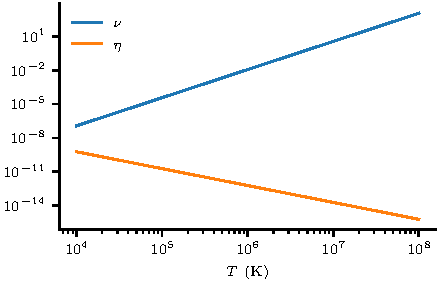
\includegraphics[width=0.5\linewidth]{visc_dep_on_temp.pdf}
  \mycaption{Dependence of non-dimensionalised viscosity $\nu$ and Spitzer resistivity $\eta$ on temperature.}{These are non-dimensionalised using typical coronal values of a magnetic field strength of $B = 5$ mT, a length of $L = 1$ Mm and a density of $\rho = 1.67 \times 10^{-12}$ kg m$^{-3}$. In the non-dimensionalisation scheme used here, the Reynolds and Lundquist numbers are the inverses of $\nu$ and $\eta$, respectively.}
  \label{fig:visc_dep_on_temp}
\end{figure}

The dominant mechanism of heat dissipation in the solar corona remains unknown, although Ohmic heating and viscous heating are two highly studied candidates. The transport parameters for viscosity $\nu$ and Spitzer resistivity $\eta$ can be derived by kinetic means as
\begin{equation}
  \label{eq:nu_and_eta}
\nu_{dim} = 10^{-17}\ T^{5/2} \text{ kg m}^{-1}\text{ s}^{-1}, \quad \eta_{dim} = 2\times 10^{9}\ T^{-3/2}\ \text{ m}^2 \text{ s}^{-1},
\end{equation}
where $T$ is the plasma temperature in Kelvin. Both expressions are taken from~\cite{braginskiiTransportProcessesPlasma1965}. Non-dimensionalising these using the scheme found in~\cite{arberStaggeredGridLagrangian2001} and typical coronal values for the Alfv\'en velocity $v_A = 3.45 \times 10^6$ m s$^{-1}$, length scale $L_0 = 1$ Mm and density $\rho_0 = 1.67 \times 10^{-12}$ kg m$^3$ give
\begin{equation}
  \label{eq:nondim_nu_and_eta}
\nu = 1.6 \times 10^{-18}\ T^{5/2} \quad \eta = 5.8 \times 10^{-4}\ T^{-3/2}.
\end{equation}
Using this non-dimensionalisation scheme the Reynolds number is given $Re = 1/\nu$ and the Lundquist number $S = 1/\eta$. Figure~\ref{fig:visc_dep_on_temp} shows the dependences of the non-dimensionalised $\nu$ and $\eta$ on temperature $T$. For a typical active region temperature of $T = 10^6$ K, $\nu \approx 10^{-3}$ and $\eta \approx 10^{-13}$.

Comparing the transport parameters for each dissipation mechanism suggests viscous heating should outperform Ohmic heating by several orders of magnitude. Indeed, many studies provide evidence to this effect~\cite{browningMechanismsSolarCoronal1991,craigViscousDissipation3D2013,craigAnisotropicViscousDissipation2009a,armstrongViscoResistiveDissipation2013,hollwegViscosityChewGoldbergerLowEquations1986a}. However, these parameters are unlikely to reflect the true degree of dissipation in the solar corona due to the influence of various effects which can enhance the effective dissipation beyond the values found via~\eqref{eq:nu_and_eta}. 

Turbulence can enhance viscosity~\cite{canutoTurbulentViscosity1988} and many mechanisms for the anomalous enhancement of resistivity have been suggested, including turbulence~\cite{cheHowAnomalousResistivity2017} and the impact of electron scattering~\cite{maEffectiveResistivityCollisionless2018}. The degree to which either dissipation mechanism is enhanced in the solar corona is difficult to estimate, however some studies have attempted to infer the effective transport parameters from observations of wave motions in coronal loops~\cite{nakariakovTRACEObservationDamped1999}, although results are disputed~\cite{klimchukCoronalSeismologyPropagation2004}. A further complication in attempting to model dissipation in the solar corona is that it is still unknown how far the collisional approximation holds~\cite{klimchukSolvingCoronalHeating2006a}.

Due to numerical diffusion present in any numerical scheme~\cite{ferzigerComputationalMethodsFluid2002}, state of the art, 3D numerical experiments are only able to probe diffusion parameters down to approximately $10^{-5}$ (non-dimensional). While this theoretically reaches the bounds of realistic viscosity, it is not close to even enhanced estimates of resistivity. Until numerical techniques and computational resources become sophisticated enough to probe realistic (enhanced or otherwise) dissipation parameters, the true nature of dissipation in the solar corona remains unclear. At best, the community can infer the importance of these and other dissipation mechanisms by constructing scaling laws for computationally feasible parameters, as is done in~\cite{craigViscousDissipation3D2013}.

\section{MHD Equations}

\subsection{The Navier-Stokes equations}

The Navier-Stokes equations are a set of partial differential equations (PDEs) which model the dynamics of a fluid through conservation of mass, momentum and energy. Generally, the equations are derived by considering conservation of the relevant quantity in a small parcel of fluid that moves with the flow. Such a derivation may be found in, for example~\cite{andersonComputationalFluidDynamics1995}. In the following description of the equations, use is made of the material derivative
\begin{equation}
  \label{eq:material_derivative}
  \frac{D}{Dt} \equiv \frac{\partial}{\partial t} + (\vec{u} \cdot \nabla)
\end{equation}
which describes the change in a quantity as it moves with flow at a velocity $\vec{u}$.

Modelling conservation of mass, the continuity equation describes the change in density $\rho$ due to the compression or dilation of the flow,
\begin{equation}
\frac{D\rho}{Dt} = - \rho \vec{\nabla} \cdot \vec{u}.
\label{eq:ns_continuity}
\end{equation}
The momentum equation is an application of Newton's second law and models the conservation of momentum in a fluid with a scalar thermal pressure $p$ and viscous stress tensor $\ten{\sigma}$,
\begin{equation}
\rho\frac{D\vec{u}}{Dt} = -\vec{\nabla} p + \vec{\nabla} \cdot \ten{\sigma}.
\label{eq:ns_momentum}
\end{equation}
The energy equation is given as
\begin{equation}
\rho\frac{D\varepsilon}{Dt} = -p \vec{\nabla} \cdot \vec{u} + \ten{\sigma} : \vec{\nabla}\vec{u},
\label{eq:ns_energy}
\end{equation}
and describes the change in internal thermal energy due to work done by pressure and viscous heating. Here, the double dot product (or tensor double contraction) is defined as $\ten{A}:\ten{B} = A_{ji} B_{ij}$ for arbitrary tensors $\ten{A}$ and $\ten{B}$. This system of equations must be closed by an additional equation of state. As presented later, the ideal equation of state is sufficient, for the purposes of describing coronal plasma.

While the Navier-Stokes equations adequately describe many fluids, conducting fluids like ionised plasmas and liquid metals couple with local magnetic fields and require an extension to the governing equations. The result are the equations of magnetohydrodynamics.

\subsection{Magnetohydrodynamics and the induction equation}

Magnetohydrodynamics (MHD) describes electrically conducting fluids, that is fluids which interact with electromagnetic fields. Typical examples of such fluids are ionised plasmas and molten metals, the investigation of the latter being key to the understanding of the Earth's molten outer core and its associated magnetic dynamo. Both small-scale laboratory plasmas, such as those found in current fusion devices, and large-scale astrophysical plasmas, such as those in the interstellar medium, can be effectively modelled using the MHD equations. While these equations have a large range of applicability, they are limited to systems with dynamics at length scales much larger than the ion skin depth or Larmor radius, and time scales much longer than the ion gyration time. For systems where the length or time scales are too small to be described by MHD, a kinetic approach using, for example, the Vlasov or Boltzmann equations is more appropriate. The ideal MHD equations can be recovered from the Boltzmann equation by taking appropriate moments~\cite{boydPhysicsPlasmas2003}.

The MHD equations are a synthesis of the Navier-Stokes equations of fluid dynamics and Maxwell's equations of electromagnetism. The latter set of equations describes the generation of an electric field $\vec{E}$ by a charge density $\rho_c$ through Gauss's law,
\begin{equation}
  \label{eq:gauss_law}
 \nabla \cdot \vec {E} ={\frac {\rho_c }{\varepsilon _{0}}},
\end{equation}
the non-existence of monopoles in the magnetic field $\vec{B}$,
\begin{equation}
  \label{eq:gauss_law_for_magnetism}
  \nabla \cdot \vec {B} =0,
\end{equation}
the generation of electric fields due to changes in the magnetic field in time $t$ through the Maxwell-Faraday equation,
\begin{equation}
  \label{eq:maxwell_faraday}
 \nabla \times \vec {E} =-{\frac {\partial \vec {B} }{\partial t}},
\end{equation}
and the generation of magnetic fields due to currents $\vec{\jmath}$ and changing electric fields through Ampère's law,
\begin{equation}
  \label{eq:ampere_law}
 \nabla \times \vec {B} =\mu _{0}\left(\vec {\jmath} +\varepsilon _{0}{\frac {\partial \vec {E} }{\partial t}}\right).
\end{equation}
Written in SI units, these equations use the permittivity $\varepsilon_{0}$ and permeability $\mu_0$ of free space.

Many conducting fluids can be considered electrically neutral, that is on the timescale of fluid motion the charges within the fluid are able to quickly redistribute to nullify any electric forces. This is true for coronal plasmas where the electrons, being much lighter than the ions, are free to quickly redistribute imbalances in charge density. This allows Gauss's law to be entirely neglected. The displacement current, the last term in Ampère's law, can also be neglected using the assumption that fluid motions are non-relativistic, that is the typical fluid velocity is much less than the speed of light, $c$~\cite{priestMagnetohydrodynamicsSuna}.

In order to couple the fluid motion to the electromagnetic fields, a constitutive Ohm's law is also included which describes the generation of currents in response to electric fields. This eventually allows the complete elimination of $\vec{E}$ from the governing equations. In a fluid's rest frame, the current response to an electric field $\vec{E}'$ is
\begin{equation}
  \label{eq:rest_frame_ohms_law}
  \vec{\jmath} = \sigma \vec{E}',
\end{equation}
where $\sigma$ is the (finite) conductivity of the fluid. The Lorentz transformation to the frame where the fluid is moving at velocity $\vec{u}$ is
\begin{equation}
  \label{eq:resistive_ohms_law}
  {\vec {E}}+{\vec{u}}\times {\vec {B}}=\eta{\vec {\jmath}},
\end{equation}
where the conductivity has been rewritten as the resistivity $\eta = 1/\sigma$. In the case of perfect conductivity, Ohm's law is written
\begin{equation}
  \label{eq:ideal_ohms_law}
  {\vec {E}}+{\vec{u}}\times {\vec {B}}=0.
\end{equation}
Additional non-ideal physics like ambipolar diffusion and the Hall effect can be modelled through additional terms in Ohm's law. However, in the solar corona these effects are small compared to resistivity and are neglected here~\cite{priestMagnetohydrodynamicsSuna}.

Combining the remaining parts of Ampère's law, the Maxwell-Faraday equation, and the resistive Ohm's law results in the induction equation,
\begin{equation}
  \label{eq:nonsimple_induction_equation}
{\frac {\partial \vec {B} }{\partial t}} = \nabla \times (\vec{u} \times \vec{B}) - \nabla \times (\eta/\mu_0 \nabla \times \vec{B}),
\end{equation}
which, in the case of uniform resistivity, may be written
\begin{equation}
  \label{eq:induction_equation}
{\frac {\partial \vec {B} }{\partial t}} = \nabla \times (\vec{u} \times \vec{B}) + \frac{\eta}{\mu_0}\nabla^2 \vec{B}.
\end{equation}
This equation essentially describes the advection and generation of a magnetic field due to fluid motions and the diffusion of the field due to resistivity. The magnetic field must still satisfy the solenoidal constraint $\nabla \cdot \vec{B} = 0$.

In order to describe the effect of the magnetic field on the fluid, additional terms must be added to the momentum~\eqref{eq:ns_momentum} and energy~\eqref{eq:ns_energy} equations. The Lorentz force describes the force exerted by the magnetic field on the fluid and is given by
\begin{equation}
  \label{eq:lorentz_force}
\vec{\jmath} \times \vec{B}.
\end{equation}
When the fluid is resistive, the dissipation of currents can heat the fluid through a process called Joule or Ohmic heating. This is modelled in the energy equation by the term
\begin{equation}
\mu_0 \eta | \vec{\jmath} |^2.
\end{equation}

\subsection{The non-dimensionalised MHD equations}

\label{sec:mhd_equations}

Combining the fluid equations~\eqref{eq:ns_continuity}--\eqref{eq:ns_energy} and the induction equation~\eqref{eq:induction_equation}, the full set of MHD equations can be written in their non-dimensionalised form
\begin{gather}
%\begin{equation}
\label{eq:mhda}
\frac{D\rho}{Dt} = - \rho \vec{\nabla} \cdot \vec{u},\\
%\end{equation}
%\begin{equation}
\rho\frac{D\vec{u}}{Dt} = -\vec{\nabla} p + \vec{\jmath} \times \vec{B} + \vec{\nabla} \cdot \ten{\sigma},\\
%\end{equation}
%\begin{equation}
\frac{D\vec{B}}{Dt} = (\vec{B} \cdot \vec{\nabla})\vec{u} - (\vec{\nabla} \cdot \vec{u})\vec{B} + \eta \nabla^2 \vec{B},\\
%\end{equation}
%\begin{equation}
\rho\frac{D\varepsilon}{Dt} = -p \vec{\nabla} \cdot \vec{u} + {Q}_{\nu} + {Q}_{\eta},%\\
\label{eq:energy}
%\end{equation}
\end{gather}
where $\eta = 1/S$ is now the non-dimensionalised resistivity, equivalent
to the inverse of the Lundquist number $S$. This notation is used throughout the remainder of this thesis. The system is closed by the inclusion of the equation of state for an ideal gas
\begin{equation}
\varepsilon = \frac{p}{\rho(\gamma - 1)},
\end{equation}
where the specific heat ratio is given by $\gamma = 5/3$. The
  terms ${Q}_{\nu} = \ten{\sigma} : \vec{\nabla}\vec{u}$ and
  ${Q}_{\eta} = \eta | \vec{\jmath} |^2$ are viscous heating and Ohmic heating, respectively.

The non-dimensionalisation scheme is identical to that used in the code Lare3d~\cite{arberStaggeredGridLagrangian2001}, where a typical magnetic field strength $B_0$, density $\rho_0$ and length scale $L_0$ are chosen and the other variables non-dimensionalised appropriately. Velocity and time are
non-dimensionalised using the Alfv\'en speed $u_A = B_0 / \sqrt{\rho_0
  \mu_0}$ and Alfv\'en crossing time $t_A = L_0/u_A$,
respectively. Temperature is non-dimensionalised via $T_0 = u_A^2
\bar{m} / k_B$, where $k_B$ is the Boltzmann constant and $\bar{m}$ is
the average mass of ions, here taken to be $\bar{m} = 1.2m_p$ (a mass
typical for the solar corona) where $m_p$ is the proton mass. Dimensional quantities can be recovered by multiplying the non-dimensional variables by their respective reference value (e.g. $\vec{B}_{\dim} = B_0 \vec{B}$). All further reference to variables will be to their non-dimensionalised values, unless stated otherwise.

\section{Anisotropic Viscosity}

Viscosity plays an important part generally in astrophysical fluid dynamics. Recent studies have demonstrated the importance of anisotropic viscosity in coronal heating in investigations of three-dimensional (3D) null points~\cite{craigViscousDissipation3D2013}, current sheet merging~\cite{armstrongViscoResistiveDissipation2013} and flux pile-up~\cite{litvinenkoViscousEnergyDissipation2005}. There is further evidence of the importance of anisotropic viscosity in other astrophysical applications including the intracluster medium~\cite{zuhoneEffectAnisotropicViscosity2014, parrishEffectsAnisotropicViscosity2012a} and the solar wind~\cite{baleMagneticFluctuationPower2009}. In other solar applications, viscosity has a role to play in the damping of coronal instabilities~\cite{howsonEffectsResistivityViscosity2017} and waves~\cite{vranjesViscosityEffectsWaves2014, erdelyiResonantAbsorptionAlfven1995a, rudermanSlowSurfaceWave2000a}, though not all these cases have been fully explored using an anisotropic model of viscosity.

\subsection{Viscosity}

Physically, viscosity is the internal friction of a fluid arising due to interactions (typically collisions) between the particles making up the fluid. Within the context of MHD, viscosity provides two functions. The first is momentum transport, included in the momentum equation as the divergence of the viscous stress tensor $\ten{\sigma}$, written using Einstein notation as
\begin{equation}
  \label{eq:viscous_momenum_transport}
  (\nabla \cdot \ten{\sigma})_j = \frac{\partial \sigma_{ij}}{\partial x_i}.
\end{equation}

In three dimensions, the nine components of $\ten{\sigma}$ quantify the flux of each component of momentum in each direction of motion as a result of viscous diffusion. For example, the $\sigma_{xy}$ component gives the flow of $x$-momentum in the $y$-direction. Due to symmetry arising from viscosity conserving angular momentum, the tensor is symmetric, so the component $\sigma_{xy}$ also quantifies the flux of $y$-momentum in the $x$-direction. Beyond the requirement of conservation of angular momentum, it is also assumed that Stokes' hypothesis holds, that is bulk viscosity is zero and viscosity does not act under uniform compression or expansion of the fluid. This requires the viscous stress tensor to be additionally trace-free,
\begin{equation}
  \label{eq:trace_free_tensor}
  \text{tr}(\ten{\sigma}) = 0.
\end{equation}
Due to the viscous stress tensor being trace-free and symmetric, the number of independent components reduces from nine to five.

The second function of viscosity is to convert kinetic into thermal energy through work done by local deformations. This is encoded in a term in the energy equation of the MHD equations of the form
\begin{equation}
  \label{eq:viscous_heat_generation}
  \ten{\sigma} : \nabla \vec{u} = \sigma_{ij} \frac{\partial u_i}{\partial x_j},
\end{equation}
and may also be written using the rate of strain tensor $\ten{W}$ as
\begin{equation}
  \label{eq:viscous_heat_generation2}
  \ten{\sigma} : \nabla \vec{u} = \frac{1}{2} \ten{\sigma} : \ten{W},
\end{equation}
where
\begin{equation}
  \label{eq:rate_of_strain}
  \ten{W} = \nabla\vec{u} + (\nabla\vec{u})^T - \tfrac{2}{3}(\nabla \cdot \vec{u})\ten{I}.
\end{equation}
The tensor $\ten{W}$ quantifies the rate at which a parcel of fluid undergoes a deformation and is symmetric and trace-free by construction.

Many fluids encountered in nature are Newtonian fluids, that is the viscous stress arising from any deformation of the fluid is directly proportional to the rate of strain of the deformation,
\begin{equation}
  \label{eq:isotropic_viscous_tensor}
  \ten{\sigma} = \nu \ten{W},
\end{equation}
where $\nu$ is the viscous transport parameter, generally referred to as the viscosity. However, in a magnetised plasma the nature of particle collisions is distinctly different from those in a non-conducting fluid and the nature of viscosity different as a result.

\subsection{Viscosity in a magnetised plasma}

\label{sec:visc_in_magnetised_plasma}

In a Newtonian fluid, the motion of a single particle travelling with typical thermal velocity $v$ and colliding with other particles in a typical collision time $\tau$ will appear as a number of broken, straight lines, each of approximate length $l = v\tau$, where $l$ is the mean free path. These motions have no preferred direction resulting in an isotropic transfer of momentum. In contrast, in a plasma made up of charged particles with charge $e$ and mass $m$, threaded by a magnetic field of strength $B$, the particles follow helical paths of approximate radius $r = v/\omega$, where $\omega = eB/m$ is the cyclotron frequency. After a time $\tau$, a typical particle will undergo a collision and its path will describe a new helix. The total resultant motion depends on the strength of the magnetic field. In the presence of a weak field, the radius of the helix may be much larger than the mean free path or in terms of the cyclotron frequency, $\omega \tau \ll 1$. As a result, the path between collisions will be close to straight and the total path will resemble that of the motion without a magnetic field. In the presence of a strong field, $\omega \tau \gg 1$ and a typical particle will be able to wind around the field a number of times, travelling a distance $l$ along the field, before colliding. As a result the transport of momentum is strongly anisotropic to the extent that it is unaffected in the direction of the field, but strongly reduced in the transverse direction.

A characteristic coronal value of $\omega \tau$ can be calculated using expressions found in Braginskii~\cite{braginskiiTransportProcessesPlasma1965}. The collision time can be written in SI units as
\begin{equation}
  \label{eq:collision_time}
  \tau = 0.82 \times 10^{-6} \frac{T^{3/2}}{n} \text{ s},
\end{equation}
where $n$ is the number density. The cyclotron frequency is written as
\begin{equation}
  \label{eq:cyclotron_frequency}
  \omega = 0.96\times10^8 B \text{ s}^{-1},
\end{equation}
where the Coloumb logarithm has been taken to be 22, and the mass fraction, the ratio of ion to proton mass, $m_f = m_i/m_p$ has been taken to be a typical solar value of $1.2$. A solar active region has typical temperatures of around $2\times 10^6$ K and number densities of $n = 3 \times 10^3\text{ m}^{-3}$, giving $\tau = 0.773$ s. The magnetic field can be as strong as $5\times 10^{-3}$ T, giving $\omega = 4.79 \times 10^5 \text{ s}^{-1}$, resulting in $\omega \tau = 3.70 \times 10^5$. Even in the quiet sun, $\omega\tau \approx 10^4$~\cite{morganGlobalConditionsSolar2017}. This indicates viscosity in most of the solar corona is highly anisotropic. 

\subsection{Anisotropic viscous tensors}

The form of the viscous stress tensor in a magnetized plasma has been derived in a number of ways to varying degrees of accuracy. The derivations typically use the methods of kinetic theory, taking moments of the Boltzmann-Maxwell equations to arrive at continuum-level approximations of the stress tensor.

A first approximation of the stress tensor can be found in the work of Chapman and Cowling~\cite{chapmanMathematicalTheoryNonuniform1970}. Their results show that the stress response to a rate of strain can be considered as responses to three types of deformation: compression or dilation along the field, deformations in the plane transverse to the field, and deformations in the plane including the field. The foremost deformation gives rise to the parallel component of viscosity, typically the largest in magnitude and often the only component modelled in applications~\cite{parrishEffectsAnisotropicViscosity2012a}. The latter two deformations give rise to two stress responses each, totalling four components: two perpendicular components and two drift components. In total there are five contributions to the viscous stress tensor in a magnetised plasma, each with an associated transport parameter. The reader is directed to a discussion by Kaufman~\cite{kaufmanPlasmaViscosityMagnetic1960} where he presents both an illustrative description of the drift and perpendicular components of the tensor, and a derivation of the full tensor from a more simplified Boltzmann equation than is used in~\cite{chapmanMathematicalTheoryNonuniform1970}. The parallel component of the stress tensor has been derived without use of kinetic theory by Hollweg~\cite{hollwegViscosityMagnetizedPlasma1985}, showing that the viscous response to parallel motions is a result of collisions repartitioning anisotropies in the thermal pressure. The tensor derived by Braginskii~\cite{braginskiiTransportProcessesPlasma1965} is perhaps the most well known and includes accurate approximations of the five viscous transport parameters.

\subsection{Simplified derivation of Braginskii tensor}

This section presents a condensed version of Braginskii's qualitative derivation of the form of the anisotropic viscosity stress tensor in a magnetized plasma, and its associated transport parameters~\cite{braginskiiTransportProcessesPlasma1965}. 

Consider a plasma where, on average, each particle moves a distance $\Delta x$ in the collision time $\tau$ before colliding. After the collision the particle has equal probability of moving to the left or the right. Since we are concerned with the viscous diffusion of momentum, and not the advection of momentum, we consider the case where the net particle flux through the plane $x=x_0$ is zero, that is the number of particles moving through the plane from the left is equal to the number of particles from the right. This implies a uniform number density in the small layer around $x_0$.

Now consider a non-uniform velocity component $u$ which changes slowly enough over the distance $\Delta x$ that we may write
\begin{equation}
  \label{eq:viscous_derivation_vy}
u (x) \approx u(x_0) + \frac{\partial u}{\partial x} \bigg| _{x_0} (x - x_0).
\end{equation}

Within a time $\tau$ half the particles in the layer between $x_0 - \Delta x$ and $x_0$ will pass through the plane $x_0$, the other half moving in the opposite direction. The flux of momentum from the left is
\begin{equation}
  \label{eq:momentum_flux_left}
F_{+} = \frac{1}{2} \int^{x_0}_{x_0 - \Delta x} \frac{1}{\tau} m n u(x) \text{d}x = \frac{mn}{2} \left[ u(x_0) - \frac{\partial u}{\partial x} \frac{\Delta x}{2} \right] \frac{\Delta x}{\tau},
\end{equation}
and the flux from the right $F_{-}$ can be calculated in a similar manner by considering the flux from the layer between $x_0$ and $x_0 + \Delta x$. The total flux of momentum moving through the point $x_0$ is
\begin{equation}
  \label{eq:total_momentum_flux}
  F = F_+ - F_- = - \nu \frac{\partial u}{\partial x}, \quad \nu \sim \frac{nm(\Delta x)^2}{\tau}.
\end{equation}
The change in momentum at the point $x_0$ is then given by the negative slope of the momentum flux $- \partial F/\partial x$. Thus, the quantity $-F$ is a measure of one component of the viscous stress tensor $\ten{\sigma}$, with the overall strength of viscous dissipation governed by the parameter $\nu$. For example, if $u$ is the velocity in the $y$-direction, $-F$ estimates the value of $\sigma_{yx}$. Substituting $\Delta x$ for appropriate lengths in the expression for $\nu$ reveals the relative strengths of the viscous response to various motions. 

In the absence of a magnetic field the viscosity is isotropic and particles are able to travel the full mean free path before colliding, hence $\Delta x = u \tau$, where $u$ is the thermal velocity. This gives an estimate for the isotropic viscous response,
\begin{equation}
  \label{eq:isotropic_eta_estimate}
  \ten{\sigma}_{iso} \sim \eta_0 \ten{W}, \quad \eta_0 \sim nm\tau v^2 \sim nT \tau,
\end{equation}
where we use the notation $\eta_0 = \nu$ here to mirror Braginskii's derivation. This should not be confused with resistivity $\eta$.

Now consider a magnetic field aligned with the $z$-direction. A similar expression to that for isotropic viscosity is found when considering the viscous response to a field-aligned gradient in a field-aligned velocity $\partial u_z / \partial z$, where $\Delta x$ is still the mean free path,
\begin{equation}
  \label{eq:parallel_eta_estimate}
\sigma_{zz} \sim \eta_0 \frac{\partial u_z}{\partial z}.
\end{equation}
That is, in a magnetised plasma, compression or dilation along the field produces the same viscous response as if the field were not there.

Now consider the same velocity $u_z$ changing in a direction perpendicular to the field, say in the $x$-direction. Then $\Delta x$ is approximately the gyroradius $r = u/\omega$. The viscous response is then
\begin{equation}
  \label{eq:perp_eta_estimate}
\sigma_{zx} \sim \eta_{\perp} \frac{\partial u_z}{\partial x}, \quad \eta_{\perp} \sim \frac{\eta_0}{(\omega \tau)^2}.
\end{equation}
A similar expression holds when a velocity perpendicular to the field, say $u_y$, varies in the $x$-direction, that is
\begin{equation}
  \label{eq:perp_eta_estimate2}
\sigma_{xy} \sim \eta_{\perp} \frac{\partial u_y}{\partial x}.
\end{equation}

The viscous response to compression or dilation perpendicular to the field arises due to a different mechanism than the simple diffusion of momentum shown previously. When the plasma is compressed or dilated perpendicular to the field, the transverse energy of the particles changes and is subsequently equipartitioned by collisions. This takes place over a finite period of time, during which the transverse and longitudinal pressures differ. This difference in pressures gives rise to a stress of the same order as the parallel contribution
\begin{equation}
  \label{eq:compression_eta_estimate}
\sigma_{xx} = \sigma_{yy} \sim \eta_0 \nabla \cdot \vec{u}, \quad \sigma_{zz} \sim - \eta_0 \nabla \cdot \vec{u}.
\end{equation}

There are further contributions to the viscous stress tensor from motions which give rise to gyroviscous stresses, the transport parameters of which vary as $\eta_0 / (\omega \tau)$. As discussed later, these contributions produce no viscous heating and shall be neglected. For a detailed discussion of these terms, see~\cite{kaufmanPlasmaViscosityMagnetic1960}.

\subsection{The Braginskii tensor}

\label{sec:braginskii_tensor}

The full Braginskii viscous stress tensor can be written in a number of ways. Braginskii's original formulation is written with the magnetic field aligned with the $z$-axis so presented here is the more general formulation of Hogan~\cite{hoganCollisionalTransportMomentum1984}, described as the sum of five tensor components $\ten{W}^{(i)}$ with associated transport parameters $\eta_i$,
\begin{equation}
\label{eq:braginskii_tensor}
\ten{\sigma}_{\text{brag}} = \eta_0 \ten{W}^{(0)} + \eta_1 \ten{W}^{(1)} + \eta_2 \ten{W}^{(2)} - \eta_3 \ten{W}^{(3)} - \eta_4 \ten{W}^{(4)}.
\end{equation}

As discussed earlier, there are three types of motion that give rise to the five tensor components: compression or dilation along the field, deformations in the plane transverse to the field, and deformations in the plane including the field. The first type of motion gives rise to the parallel term,
\begin{equation}
  \label{eq:braginskii_parallel_term}
  \ten{W}^{(0)} = \frac{3}{2}(\ten{W}\vec{b}\cdot\vec{b}) \left( \vec{b} \otimes \vec{b} - \frac{1}{3}\ten{I} \right),
\end{equation}
where $\vec{b} = \vec{B}/|\vec{B}|$ is the unit vector in the direction of the field. The second and third types of motion give rise to two types of stress: two perpendicular terms,
\begin{align}
\ten{W}^{(1)} &= (\ten{I} - \vec{b} \otimes \vec{b})\ten{W}(\ten{I} - \vec{b} \otimes \vec{b}) + \frac{1}{2}(\ten{W}\vec{b} \cdot \vec{b})(\ten{I} - \vec{b} \otimes \vec{b}), \\
\ten{W}^{(2)} &= (\ten{I} - \vec{b} \otimes \vec{b})\ten{W}(\vec{b} \otimes \vec{b}) + (\vec{b} \otimes \vec{b})\ten{W}(\ten{I} - \vec{b} \otimes \vec{b}),
\end{align}
and two terms often called the drift or gyroviscous terms,
\begin{align}
\ten{W}^{(3)} &= \frac{1}{2} \ten{Z}\ten{W}(\ten{I} - \vec{b} \otimes \vec{b}) - \frac{1}{2}(\ten{I} - \vec{b} \otimes \vec{b})\ten{W}\ten{Z}, \\
\ten{W}^{(4)} &= (\ten{Z}\ten{W}\vec{b}) \otimes \vec{b} + \vec{b} \otimes (\ten{Z} \ten{W} \vec{b}),
\label{eq:drift_terms}
\end{align}
where the tensor $\ten{Z}$ has components $Z_{ij} = \varepsilon_{ikj}b_k$, where $\varepsilon_{ikj}$ is the Ricci alternating tensor (note the index ordering). It can be shown that these five tensors are mutually orthogonal, that is $\ten{W}^{(i)}:\ten{W}^{(j)} = 0$ for $i\ne j$.

Braginskii derives the five viscosity coefficients $\eta_i$ from a kinetic description of the plasma (see~\cite{epperleinPlasmaTransportCoefficients1986} for an example derivation). While more modern methods of deriving transport parameters have generally produced more accurate estimates~\cite{epperleinPlasmaTransportCoefficients1986}, Braginskii's expressions combine relative simplicity and good accuracy are are still widely used. These are the expressions used throughout this thesis.

The parallel viscosity coefficient $\eta_0$ is identical to the dynamic viscosity coefficient of an unmagnetised plasma $\nu$ and has already been given in expression~\eqref{eq:nu_and_eta}. For completeness, this is restated here,
\begin{equation}
\label{eq:nu}
\eta_0 = 0.68 \times 10^{-16} T^{5/2} \text{ kg m}^{-1} \text{ s}^{-1}.
\end{equation}

\begin{figure}[t]
  \centering
  \includegraphics[width=0.5\linewidth]{brag_coeffs.pdf}
  \mycaption{Dependence of Braginskii coefficients $\eta_1$ and $\eta_3$ on magnetic field strength.}{The collision time is $\tau = 0.77$ s, corresponding to a typical coronal temperature of $T=10^6$ K. Both expressions are normalised against $\eta_0$.}
\label{fig:visc_dep}%
\end{figure}

For simplicity, the dimensionless quantity $x = \omega \tau$ is used in the expressions for the remaining transport parameters, as is done in~\cite{braginskiiTransportProcessesPlasma1965}, and all coefficients have identical units to $\eta_0$. The two perpendicular coefficients are written,
\begin{equation}
  \label{eq:perp_visc_coeff}
  \eta_2(x) = \frac{\eta_0}{\Delta} \left( \tfrac{6}{5} x^2 + 2.23 \right), \quad \eta_1 = \eta_2(2x),
\end{equation}
where
\begin{equation}
  \label{eq:delta}
\Delta = x^4 + 4.03x^2 + 2.23.
\end{equation}
The drift coefficients are written,
\begin{equation}
  \label{eq:drift_visc_coeff}
  \eta_4(x) = \frac{\eta_0}{\Delta} x \left( x^2 + 2.38 \right), \quad \eta_3 = \eta_4(2x).
\end{equation}
The relative strength of the five coefficients is important in considering which are most significant in the solar corona. The drift coefficients are of the order $\eta_0/(\omega \tau)$ and the perpendicular coefficients of the order $\eta_0/(\omega \tau)^2$. The dependence on the magnetic field strength can be seen in figure~\ref{fig:visc_dep}.

As has already been discussed, the origin of each of the five viscosity components can be understood by considering the effect of velocity gradients and collisions on a plasma from a kinetic perspective. The drift terms are products of the velocity gradient perturbing particle orbits which generates pressure anisotropies and, in the absence of collisions, produces a stress which is orthogonal to the strain, resulting in no viscous dissipation. Collisions repartition the anisotropies in the pressure giving rise to the perpendicular terms. This is explored in detail by Kaufman in~\cite{kaufmanPlasmaViscosityMagnetic1960}. 

While it is illustrative to understand from a kinetic perspective why the drift terms produce no dissipation, it can be shown explicitly for the terms given in equation~\eqref{eq:drift_terms}. The strain rate tensor can be written as the sum of only the parallel and perpendicular terms, $\ten{W} = \ten{W}^{(0)} + \ten{W}^{(1)} + \ten{W}^{(2)}$. Since the drift terms are individually orthogonal to $\ten{W}^{(0)}$, $\ten{W}^{(1)}$ and $\ten{W}^{(2)}$, they are also orthogonal to $\ten{W}$. By equation~\eqref{eq:viscous_heat_generation2}, the drift terms cannot contribute to overall viscous dissipation. Furthermore, the relative size of the transport coefficients ($\eta_3 \propto \eta_0/(\omega\tau)$) suggests the drift terms may be completely neglected. While these terms can still meaningfully participate in certain dynamics~\cite{dellarPlanarChannelFlow2011,ferraroFiniteElementImplementation2006}, this thesis focuses on the impacts of viscosity on coronal heating and so the drift terms will be neglected throughout the remainder of this work. While a similar argument suggests the perpendicular terms should also be neglected ($\eta_1 \propto \eta_0/(\omega\tau)^2$), they are required to rewrite the Braginskii tensor in a form useful for numerical simulation, as discussed later.

\subsection{Limit of strong magnetic field}

As already mentioned, in an solar active region $\omega \tau \approx 10^5 \gg 1$ and the transport coefficients in equations~\eqref{eq:perp_visc_coeff} and~\eqref{eq:drift_visc_coeff} become negligibly small compared to the parallel coefficient. As a result, in the absence of any magnetic null points, the Braginskii tensor can be reduced to its strong-field approximation,
\begin{equation}
  \label{eq:strong_field_approx}
\ten{\sigma}_{\text{brag}} = \eta_0 \ten{W}^{(0)} = \tfrac{3}{2} \eta_0 (\ten{W} \vec{b} \cdot \vec{b}) ( \vec{b} \otimes \vec{b} - \tfrac{1}{3} \ten{I}).
\end{equation}
In a local coordinate system where the magnetic field is aligned with $\vec{e}_z$, the tensor is
\begin{equation}
  \label{eq:z_aligned_strong_field_approx}
\ten{\sigma}_{\text{brag}} = \tfrac{3}{2} \eta_0 W_{zz} ( \vec{e}_z \otimes \vec{e}_z - \tfrac{1}{3} \ten{I}),
\end{equation}
where $\vec{e}_z$ is the unit vector in the $z$-direction. Notice that the only velocity gradient to enter into the above tensor is that which is aligned with the magnetic field (including gradients stemming from the compressional $\nabla \cdot \vec{u}$ term in the rate of strain tensor, equation~\eqref{eq:rate_of_strain}). It can also be seen that the magnetic field has no effect on the component of viscosity parallel to the field; it is identical to the corresponding component in the isotropic stress tensor,
\begin{equation}
  \label{eq:z_aligned_iso}
  (\sigma_{\text{iso}})_{zz} = (\sigma_{\text{brag}})_{zz} = \eta_0 W_{zz}.
\end{equation}
In the strong-field regime, the only motion damped by viscosity is non-uniform compression or dilation of the plasma. 

This approximation is valid even for quiet Sun conditions, where $\omega\tau \approx 10^4$. Where this approximation fails is around magnetic null points, regions of the corona where the magnetic field vanishes. Null points are an important, abundant feature in the coronal magnetic field~\cite{edwardsNullPointDistribution2015} and participate in a number of important solar phenomena~\cite{massonNATUREFLARERIBBONS2009,moreno-insertisPLASMAJETSERUPTIONS2013,barnesRelationshipCoronalMagnetic2007}. Any general model of solar viscosity must go beyond the strong-field approximation and additionally incorporate viscosity in the limit of weak magnetic field.

\subsection{Limit of weak magnetic field}

While the full Braginskii tensor~\eqref{eq:braginskii_tensor} presents the natural separation of viscous responses into parallel, perpendicular and drift components, this form is unsuitable for numerical simulation when null points are present in the magnetic field. As the field strength goes to zero approaching a null point, the unit vector $\vec{b}$ in equations~\eqref{eq:braginskii_parallel_term}--\eqref{eq:drift_terms} becomes mathematically undefined. Numerically, the calculation of $\vec{b}$ involves division by the magnitude of the field which is a quantity close to or exactly zero near a null point, leading to errors or complete failure of the numerical scheme. Even if a numerical implementation were to check for a locally small field, it's unclear how the viscous terms and transport coefficients, as written in the form of equation~\eqref{eq:braginskii_tensor}, interact as the field strength tends to zero. By rewriting the tensor as
\begin{eqnarray}\label{eq:brag_new}
\ten{\sigma}_{\rm brag} = &&\frac{3\eta_0+\eta_1-4\eta_2}{2|\vec{B}|^4}(\ten{W}\vec{B}\cdot\vec{B})(\vec{B}\otimes\vec{B})\\
\nonumber
& &+~ \frac{\eta_1-\eta_0}{2|\vec{B}|^2}(\ten{W}\vec{B}\cdot\vec{B})\ten{I}\\
\nonumber
& &+~ \frac{\eta_2-\eta_1}{|\vec{B}|^2}[\ten{W}(\vec{B}\otimes\vec{B})+(\vec{B}\otimes\vec{B})\ten{W}] \\
\nonumber
& &+~ \eta_1\ten{W},
\end{eqnarray}
the anisotropic terms and isotropic term are clearly separated. The grouping of terms and the explicit use of $\vec{B}$ rather than $\vec{b}$ allows a numerical implementation to check the local value of $|\vec{B}|$ and, if it's smaller than some threshold, manually set the anisotropic coefficients in equation~\eqref{eq:brag_new} to zero, avoiding a division by $|\vec{B}|$.

Similar to the strong-field limit, it can be shown that the magnetic field in the weak-field limit has no effect on the field-aligned component of momentum transport in~\eqref{eq:brag_new}. That is, ~\eqref{eq:z_aligned_iso} still holds.

\section{Conclusion}

This chapter introduces the layers of the Sun, in particular the solar corona, and summarises some recent developments in coronal heating. The MHD equations are presented as a synthesis of the Navier-Stokes equations of fluid dynamics and Maxwell's equations of electromagnetism and are non-dimensionalised. Viscosity in a magnetised plasma is discussed in detail and the particular nature of viscosity in the solar corona is explored. This general introduction to the solar atmosphere provides the foundation upon which the remainder of the thesis is built.

\chapter{Numerical methods}

\label{chp:numerical_methods}

\graphicspath{{images/numerical_methods/}}

This chapter introduces the main numerical method used in the rest of the thesis, the Lagrangian-remap scheme used in the 3D MHD code Lare3d. This is done through the development of a 1D, hydrodynamic implementation of the scheme. The discretisation and time-stepping algorithms are described, along with the shock capturing techniques used, and the application to 3D MHD summarised. Finally, the Sod shock problem is used to compare the results of the code against an analytical solution. The results of a parameter search for optimal shock viscosity values is given and the results of a convergence study presented.

\section{Lare1d}

Lare3d, an abbreviation of LAgragian-REmap 3D, is a 3D MHD code which employs the Lagrangian-remap scheme, a form of numerical scheme used to solve hyperbolic partial differential equations like those often found in hydrodynamics (HD) and MHD. The core idea of the scheme is to solve the equations on a grid in Lagrangian form, which involves a deformation of the grid, and then to remap the variables back to the original grid. This two-step process, combined with additional shock-capturing techniques such as flux limiters and shock viscosity, is extremely effective at capturing the kind of shocks that are generated in highly compressible, dynamic coronal simulations. It compares well to Roe solvers when solving identical problems~\cite{arberStaggeredGridLagrangian2001}.

As a consequence of the Lagrangian step, the equations are solved in a much simpler form than if they were to be solved in equivalent Eulerian form, removing some of the nonlinearity found in the Eulerian description. The disadvantage of this is that a complex remap step must be introduced. However, once the remap problem is solved (and it is only a complicated but tractable problem of geometry) it is not necessary to change the step if the physics are changed. Like other finite-volume methods, the method requires only local communication, that is a computation on a single cell requires only information from neighbouring cells. This locality reduces the overhead associated with communication between nodes when implementing the method on large clusters and makes the method viable for large-scale, parallel simulations. 

This section presents the implementation and testing of a 1D Lagrangian-remap scheme applied to the inviscid, compressible Euler equations. Then a summary is provided of the MHD code Lare3d~\cite{arberStaggeredGridLagrangian2001} which is used to perform the numerical experiments detailed in the rest of the thesis. 

\subsection{The physical model}

Flows of an ideal, inviscid fluid can be described using the Euler equations, here in 1D. The continuity equation describes the change in density $\rho$ due to expansion or compression of the fluid through spatial change in the flow velocity $u$,
\begin{equation}
  \frac{D \rho}{Dt} + \rho\frac{\partial u}{\partial x} = 0.\\
  \label{eqn-Lare1d-density}
\end{equation}
The momentum equation describes the change in velocity due to a difference in pressure $p$,
\begin{equation}
  \frac{D u}{Dt} + \frac{1}{\rho}\frac{\partial p}{\partial x} = 0.\\
  \label{eqn-Lare1d-velocity}
\end{equation}
The energy equation describes the change in internal energy $\varepsilon$ due to expansion or compression,
\begin{equation}
  \frac{D \varepsilon}{Dt} + \frac{p}{\rho}\frac{\partial u}{\partial x} = 0,\\
  \label{eqn-Lare1d-energy}
\end{equation}
and finally the system is closed using the equation of state for an ideal gas,
\begin{equation}
  p = \varepsilon\rho(\gamma - 1).
  \label{eqn-Lare1d-equation-of-state}
\end{equation}
Use has been made of the Lagrangian derivative, defined as
\begin{equation}
  \frac{D }{Dt} \equiv \frac{\partial}{\partial t} + (\vec{u} \cdot \nabla),
\end{equation}
which describes the change in a quantity within a parcel of fluid as that parcel is advected by the flow. 

\subsection{Discretisation} 

\begin{figure}[t]
    \hfill
    \begin{subfigure}{0.3\textwidth}
      \centering
      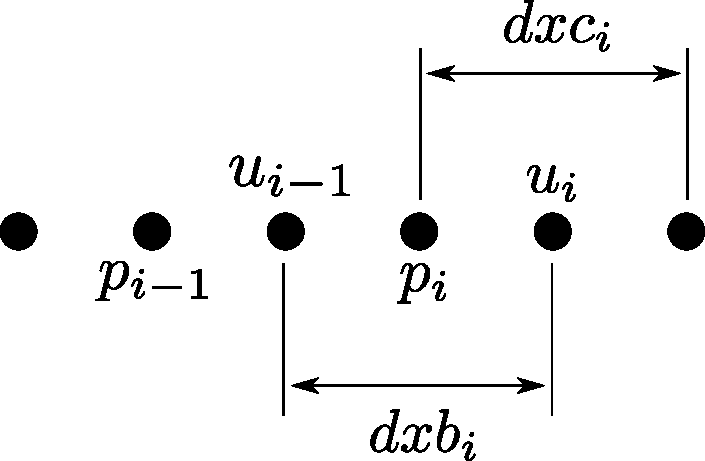
\includegraphics[width=1.0\linewidth]{staggered_grid.pdf}
      \caption{Staggered grid}%
      \label{fig:staggered_grid}
    \end{subfigure}
    \hfill
    \begin{subfigure}{0.49\textwidth}
      \includegraphics[width=\linewidth]{remap.png}
      \caption{Deformation and remap of the grid}%
      \label{fig:remap}
    \end{subfigure}
    \mycaption{Illustrations of the staggered grid and its deformation.}{In~\ref{fig:staggered_grid} the staggered grid is illustrated with velocity located at cell-boundaries and pressure located at cell-centres. Illustrated in~\ref{fig:remap} is the deformation of the grid during the Lagrangian step and the remapping of variables back to the original grid during the remap step.}
\label{fig:grid_and_remap}%
\end{figure}

As illustrated in figure~\ref{fig:staggered_grid}, the grid on which the variables are defined is staggered, that is the velocity is defined at the boundary of the cells, and all other variables are defined at cell centres. This is in contrast to collocated grids where all variables are defined at the same locations on a single grid. Without staggering, the specific choice of the spatial discretisation of derivatives would result in two sets of decoupled equations, one associated with even indices and one with odd. This decoupling can cause a numerical instability often called the checkerboard problem and is a common numerical issue generally in computational fluid dynamics~\cite{ferzigerComputationalMethodsFluid2002}. Additionally, the use of a staggered grid can improve the accuracy of a finite-difference scheme with little extra computational overhead~\cite{rojanaratanangkulePerformanceHighOrder2015}. However, a staggered grid is more complex to implement, requiring careful consideration of the precise locations of derivatives and the handling of two separate grids. 

Due to the staggered grid, the derivative of the velocity is defined at the centre of a cell as the first-order, central finite-difference of the velocity at the boundaries,
\begin{equation}
  {\left( \frac{\partial u}{\partial x} \right)}_i = \frac{u_i - u_{i-1}}{dxb_i},
  \label{}
\end{equation}
and similarly the derivative of pressure (or any of the other cell-centred variables) is defined at the boundaries as
\begin{equation}
  {\left( \frac{\partial p}{\partial x} \right)}_i = \frac{p_i - p_{i-1}}{dxc_i}.
  \label{}
\end{equation}

\subsection{The Lagrangian step}
The Lagrangian step uses a kind of predictor-corrector scheme to advance the system one timestep\footnote{It is unclear whether this type of numerical integration scheme could be considered a ``true'' predictor-corrector scheme or a form of explicit Runge-Kutta method. Predictor-corrector schemes typically provide a prediction of the system at a single advanced timestep using an explicit method and then correct the values at that timestep using an implicit method~\cite{butcherNumericalMethodsOrdinary2004}. In contrast, an explicit Runge-Kutta scheme advances the system using multiple approximate solutions at intermediate timesteps. It is my opinion that this scheme is better described as a Runge-Kutta method however the full 3D MHD code, Lare3d, and its corresponding literature~\cite{arberStaggeredGridLagrangian2001} use predictor-corrector nomenclature, so those terms are used here for consistency with~\cite{arberStaggeredGridLagrangian2001}.}. Each timestep is split into two substeps, the first calculating an approximation of the pressure, and the second using this pressure to advance all other variables to the next full timestep. Here, the current timestep is denoted as timestep $n$, the predictor step advances the pressure to timestep $n+1/2$ and then finally the corrector step advances the remaining variables to timestep $n+1$.

\paragraph{The predictor step}
It can be shown by Taylor expansion \todo{show this via taylor expansion?} that calculating $u^{n+1}$, $\varepsilon^{n+1}$ and $\rho^{n+1}$ to second order only requires calculating $p^{n+1/2}$ to first order. Using~\eqref{eqn-Lare1d-equation-of-state},
\begin{equation}
  p_i^{n+1/2} = \varepsilon_i^{n+1/2}(\gamma-1)\rho_i^{n+1/2}.
  \label{eqn-predictor-pressure}
\end{equation}
The energy density at the half timestep is calculated from the discretisation of~\eqref{eqn-Lare1d-energy},
\begin{equation}
  \varepsilon_i^{n+1/2} = \varepsilon_i^{n} - \frac{dt}{2} \frac{1}{\rho_i^n} \frac{u_i^n - u_{i-1}^n}{dxb_i^n}p_i^{n+1/2}.
  \label{eqn-predictor-energy}
\end{equation}
Since mass is conserved, the change in density in a cell is related to the change in volume of that cell in the following way,
\begin{equation}
  \rho_i^{n+1} = \frac{\rho_i^{n}}{\Delta_i},
\end{equation}
where $\Delta_i = dxb_i^{n+1}/dxb_i^{n}$ is the fractional change in volume of cell $i$ between current and future timesteps. In this case, the density at the half timestep is found by calculating the updated grid boundary separation, again at the half timestep,
\begin{equation}
  dxb_i^{n+1/2} = dxb_i^n + \frac{dt}{2}(u_i^n - u_{i-1}^n).
  \label{eqn-predictor-boundary-distance}
\end{equation}
This is fed into the calculation of the change in volume to give the updated density,
\begin{equation}
  \rho_i^{n+1/2} = \rho_i^n \frac{dxb_i^n}{dxb_i^{n+1/2}}.
  \label{eqn-predictor-density}
\end{equation}

\paragraph{The corrector step}
\label{sec-corrector-step}
After the half timestep pressure has been calculated, the velocity, energy and grid spacing are all advanced to time index $n+1$. The velocity is updated through the discretisation of~\eqref{eqn-Lare1d-velocity},
\begin{equation}
  u_i^{n+1} = u_i^n - dt \frac{1}{\rho^n_{i+1/2}}\frac{p^{n+1/2}_{i+1} - p^{n+1/2}_i}{dxc_i^n},
  \label{}
\end{equation}
where the density at the cell boundary $\rho_{i+1/2}$ is found via a mass-conserving interpolation,
\begin{equation}
  \rho_{i+1/2} = \frac{dxb_i \rho_i + dxb_{i+1}\rho_{i+1}}{dxb_i + dxb_{i+1}}.
  \label{eqn-lagrangian-density-interpolation}
\end{equation}
Since the product $\rho_i dxb_i$ is conserved throughout the Lagrangian step, that is $\rho_i^{n+1/2} dxb_i^{n+1/2} = \rho_i^n dxb_i^n$, values at timestep $n$ are used in~\eqref{eqn-lagrangian-density-interpolation}.

In order to advance the remaining variables the half timestep value for the velocity is required, calculated using a simple average between current and future timesteps,
\begin{equation}
  u_i^{n+1/2} = \frac{1}{2}(u_i^{n} + u_i^{n+1}).
  \label{}
\end{equation}
This allows the advancement of the energy to the next full timestep, calculated from the discretisation of~\eqref{eqn-Lare1d-energy},
\begin{equation}
  \varepsilon_i^{n+1} = \varepsilon_i^{n} - dt \frac{1}{\rho_i^n} \frac{u_i^{n+1/2} - u_{i-1}^{n+1/2}}{dxb_i^n}p_i^{n+1/2}.
  \label{}
\end{equation}
The grid separation is updated,
\begin{align}
  dxb_i^{n+1} &=  dxb_i^n + dt(u_i^{n+1/2} - u_{i-1}^{n+1/2}),\\
  dxc_i^{n+1} &=  (dxb_i^{n+1} + dxb_{i+1}^{n+1})/2,
  \label{eqn-lagrangian-grid-update}
\end{align}
and finally the density updated,
\begin{equation}
  \rho_i^{n+1} = \rho_i^n \frac{dxb_i^n}{dxb_i^{n+1}}.
  \label{}
\end{equation}

\subsection{The remap step}
The Lagrangian step distorts the grid from its original state. The remap step rectifies this by mapping the variables from the distorted Lagrangian grid to the original, undeformed grid. Initially the density is remapped using regular coordinates before switching to a mass coordinate to remap the energy and velocity. Using change of coordinate has the benefit of conserving mass during the remap step.

The remapping process is a purely geometrical exercise; the problem-specific physics are contained entirely in the Lagrangian step. This is advantageous when applying the scheme to a general set of problems since once the remap step is realised and implemented, the entire scheme can be adapted to a specific problem by changing only the equations in the Lagrangian step. Major changes in geometry such as a different coordinate system or the inclusion of different boundary conditions may require some adaptation in the remap step. Although the implementation detailed in this chapter (and that of Lare3d) takes one Lagrangian step per remap step, some implementations of similar schemes take many Lagrangian steps, continuing until the distortion of the grid becomes greater than some criteria, only then performing a remap step. The following remap process could be used to remap a distortion created over multiple Lagrangian steps and only requires data from before and after the entire deformation of the grid. 

\paragraph{The Density Remap}

\begin{figure}[t]
  \centering
  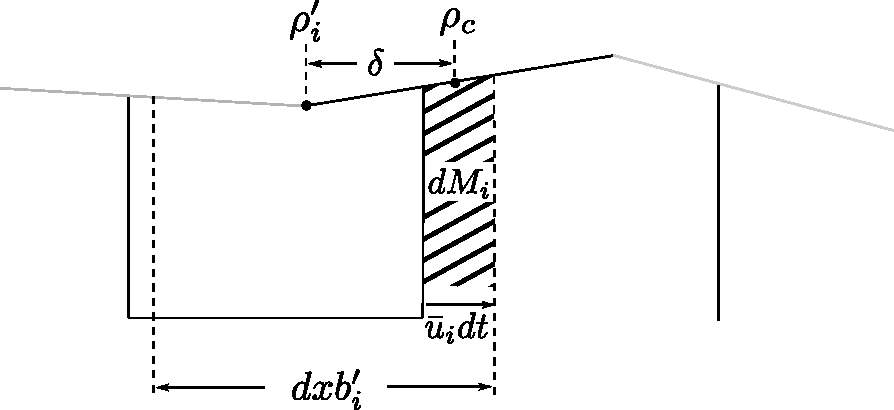
\includegraphics[width=0.7\linewidth]{mass_movement.pdf}
  \mycaption{Advection of mass from one cell to an adjacent cell.}{}%
  \label{fig:mass_movement}
\end{figure}

During a single Lagrangian step an amount of mass $dM_i$ leaves the $i$-th Eulerian cell via the right hand side and an amount $dM_{i-1}$ enters via the left hand side, as illustrated in figure~\ref{fig:mass_movement}. The mass remaining in the cell is given by
\begin{equation}
  \rho^{n+1}_i dxb_i = \rho'_i dxb'_i - dM_i + dM_{i-1},
  \label{eqn-remap-mass-in-cell}
\end{equation}
where $\rho_i$ without the dash denotes the density before the Lagrangian step, $\rho'_i$ denotes the density of the $i$-th cell after a Lagrangian step (but before the remap step) and $\rho_i^{n+1}$ to denote the final density after the remap step. Note that the grid spacing is remapped to its original Eulerian value so $dxb^{n+1}_i = dxb_i$. By conservation of mass during the Lagrangian step, $\rho_i dxb_i = \rho'_i dxb'_i$ and~\eqref{eqn-remap-mass-in-cell} becomes
\begin{equation}
  \rho^{n+1}_i = \rho_i + \frac{1}{dxb_i} (dM_{i-1} - dM_i).
  \label{eqn-remap-density}
\end{equation}

As illustrated in figure~\ref{fig:mass_movement}, $\rho_i$ is considered piecewise linear which allows the approximation of the movement of mass as
\begin{equation}
  dM_i = \rho_c \bar{u}_i dt,
\end{equation}
where $\bar{u}_i = u_i^{n+1/2}$ denotes the velocity of the boundary (as in~\eqref{eqn-lagrangian-grid-update}). The density of the portion of the cell which has moved beyond the right hand side boundary is given by
\begin{equation}
  \rho_c = \rho_i' + \delta \frac{\partial \rho_i'}{\partial x'}.
\end{equation}
Geometrically it can be seen that,
\begin{align}
  \delta =  \frac{1}{2} dxb_i' - \frac{1}{2} \bar{u}_i dt = \frac{1}{2} dxb_i'(1-\psi),
\end{align}
where $\psi = \bar{u}_i dt / dxb_i'$. The calculation of $\partial\rho_i'/ \partial x'$ is performed using a third-order upwind method given by
\begin{equation}
  \label{eq:upwind_method}
\frac{\partial \rho_i'}{\partial x'} = 
\begin{cases}
\frac{2-\psi_i}{3} \frac{\rho_{i+1} - \rho_i}{dxb_i} + \frac{1+\psi_i}{3}\frac{\rho_i - \rho_{i-1}}{dxb_{i-1}}, \quad \bar{u_i} > 0,\\
\frac{2-\psi_i}{3} \frac{\rho_{i+1} - \rho_i}{dxb_i} + \frac{1+\psi_i}{3}\frac{\rho_{i+2} - \rho_{i+1}}{dxb_{i+1}}, \quad \bar{u_i} \leq 0.
\end{cases}
\end{equation}
The corresponding method for variables located at the boundaries uses a similar formula but with $dxb$ replaced by $dxc$. As is explained in section~\ref{sec:shock_capturing}, the naive application of this method can lead to numerical issues so, in practice, the gradient is limited using the flux limiter described in section~\ref{sec-flux-limiters}. The mass leaving the right hand side is calculated as
\begin{equation}
dM_i = \left( \rho_i' + \frac{1}{2}dxb'_i(1-\psi) \frac{\partial \rho_i'}{\partial x'} \right) \bar{u}_i dt,
\label{eqn-remap-mass-diff}
\end{equation} 
and feeding that into~\eqref{eqn-remap-density} completes the density remap.

\subsection{The Specific Energy Density Remap}
At this point in the algorithm, the mass leaving the $i$-th cell $dM_i$ has already been calculated and this is used to form a change of coordinates, from $x$-coordinates to mass coordinates, denoted by $\xi$, which is used to remap the remaining variables. The distance $dxb_i$ can be written in mass coordinates as
\begin{equation}
\label{eqn-change-of-coord}
  d\xi_i = \rho_i dxb_i = \rho_i' dxb_i'.
\end{equation}
In this coordinate, $dM_i$ directly measures the degree to which the right hand side of the boundary of cell $i$ has moved during a Lagrangian step.

\begin{figure}[t]
  \centering
  \includegraphics[width=0.7\linewidth]{energy_movement.pdf}
  \mycaption{Advection of energy from one cell to an adjacent cell.}{}%
  \label{fig:energy_movement}
\end{figure}

The energy remap now follows a similar path to the density remap. By analogy with~\eqref{eqn-remap-mass-in-cell}, the energy remaining in the $i$-th cell after a Lagrangian step is given by
\begin{equation}
  \varepsilon_i^{n+1} d\xi_i^{n+1} = \varepsilon_i' d\xi_i' + dE_{i-1} - dE_i,
\end{equation}
where $dE_i$ is the amount of energy being advected out of the cell through the right hand side boundary and $dE_{i-1}$ is the energy advected in through the left hand side boundary. Rearranging for $\varepsilon_i^{n+1}$, 
\begin{equation}
  \varepsilon_i^{n+1}  = \frac{1}{d\xi_i^{n+1}}(\varepsilon_i'd\xi_i' + dE_{i-1} - dE_i).
  \label{eqn-remap-specific-energy-density}
\end{equation}
At this point, only the calculation of $dE_i$ is unknown and can be found by analogy to the density remap by considering figure~\ref{fig:energy_movement}. In mass coordinates,
\begin{equation}
  dE_i = \varepsilon_c dM_i,
\end{equation}
where
\begin{equation}
  \varepsilon_c = \varepsilon_i' + \delta \frac{\partial \varepsilon_i'}{\partial \xi},
\end{equation}
and
\begin{equation}
  \delta = \frac{1}{2}d\xi_i - \frac{1}{2}dM_i.
\end{equation}
Hence, 
\begin{equation}
  dE_i = \left( \varepsilon_i' + \frac{1}{2}\frac{\partial \varepsilon_i'}{\partial \xi} (d\xi_i - dM_i) \right)dM_i.
\end{equation}
To convert from mass coordinates, use is made use of the chain rule,
\begin{equation}
  d\xi_i \frac{\partial \varepsilon_i'}{\partial \xi} = dxb_i\rho_i \frac{\partial \varepsilon_i'}{\partial \xi} = dxb_i \frac{\partial \varepsilon_i'}{\partial x}
\end{equation}
to rewrite $dE_i$ as
\begin{equation}
  dE_i = \left( \varepsilon_i' + \frac{1}{2}dxb_i\frac{\partial \varepsilon_i'}{\partial x} \left( 1 - \frac{dM_i}{\rho_i dxb_i} \right) \right)dM_i,
  \label{eqn-remap-energy-difference}
\end{equation}
where, in practice, calculation of $\partial \varepsilon_i'/\partial\xi$ is again performed using a flux limiter (discussed in section~\ref{sec-flux-limiters}). Feeding this final equation into~\eqref{eqn-remap-specific-energy-density} completes the specific energy density remap.

\subsection{The velocity remap}
\label{sec-remap-velocity}
The velocity remap is nearly identical to the specific energy density remap shown previously so a derivation will not be given, however since the velocity is defined at cell centres, some of the relevant variables must be interpolated. The final two equations required to remap the velocity are 
\begin{align}
  dU_i &= \left( u_i' + \frac{1}{2}dxc_i\frac{\partial u_i'}{\partial x} \left( 1 - \frac{dM_{i+1/2}}{\rho_{i+1/2} dxc_i} \right) \right)dM_{i+1/2},\\
  u_i^{n+1}  &= \frac{1}{dxc_i \rho_{i+1/2}^{n+1}}(u_i' dxc_i \rho_{i+1/2} + dU_{i-1} - dU_i),
\end{align}
where the boundary distance $dxb$ is replaced by the cell centre distance $dxc$, mass is interpolated using an average, $dM_{i+1/2} = (dM_{i} + dM_{i+1})/2$, and the density is interpolated using equation \eqref{eqn-lagrangian-density-interpolation}. Once again, the derivative $\partial u_i' / \partial x$ is found using a flux limiter. 

\subsection{Constraints on the timestep}
Lagrangian-remap schemes are often considered to be unconditionally stable and do not have a CFL condition like many explicit numerical schemes~\cite{batesMultiplyUpstreamSemiLagrangianAdvective1982}. Despite this, the remap step detailed previously makes some assumptions about how the grid deforms during the Lagrangian step, namely a gridpoint cannot be advected more than one grid separation away from its original position. This condition appears similar to a CFL condition and restricts the timestep $dt$ to
\begin{equation}
  \label{eq:grid_condition1}
  dt < \frac{dxb_i}{|u_i|}\quad \forall i.
\end{equation}
Without this condition a large enough velocity could deform the grid so much that the remap step is not able to correctly remap the variables. With a more complex remap step, the assumptions about the grid deformation and corresponding timestep constraints could be relaxed.

\subsection{Language and library choice}
This example of a LARE scheme was implemented in C++, a language which effectively balances computational speed and usability. The \emph{getopt} and \emph{json} libraries were used to take input from a JSON file allowing for better runtime flexibility. The unit testing library \emph{Catch} was used as the testing framework. Since this is a one-dimensional problem with limited complexity, there was no need to include parallelism in the code, although due to the computations being well-localised, it would be reasonably simple to parallelise the code using similar approaches to those commonly applied to finite-difference and finite-volume codes. Some helper tools were also written in Python and running scripts in bash. Due to the mature numerical and plotting libraries available for Python, it is a natural choice of language for developing tools.

\section{Shock capturing techniques}
\label{sec:shock_capturing}

In hyperbolic systems of PDEs such as that given in equations~\eqref{eqn-Lare1d-density}--\eqref{eqn-Lare1d-energy} solutions may contain discontinuities like shock waves (also known as shocks). While such shocks do have some physical width in real systems, they are typically so thin compared to the larger scales of the system they are treated as mathematical discontinuities. Numerical solvers which aim to represent a solution on a finite grid of points struggle to provide adequate resolution to accurately resolve a shock. When under-resolved, high-resolution numerical solvers may overestimate the shock, creating an overshoot in the solution and introducing spurious oscillations in the wake of the shock, known as the carbuncle phenomenon~\cite{rodionovArtificialViscosityCure2019}. Two methods of dealing with these unwanted oscillations are used in this code: flux limiters, which restricts spatial gradients and maintains monotonicity, and shock viscosity, which acts to better resolve the shock by spreading it over numerous grid points. The use of these techniques in both the 1D code and Lare3d are detailed here.

\subsection{Flux Limiters}
\label{sec-flux-limiters}

Flux limiters are numerical tools applied to high-resolution schemes to reduce the spurious oscillations associated with such schemes by restricting the flux through some numerical interface. In practice, this often involves the restriction of spatial gradients, so flux limiters are often called slope limiters. A wide variety of flux limiters have been developed, however attention here is restricted to total variation diminishing (TVD) schemes, specifically that of van Leer~\cite{vanleerUltimateConservativeDifference1997}. For a review of other TVD schemes, see~\cite{zhangReviewTVDSchemes2015}, and for a review of the related essentially non-oscillatory scheme, see~\cite{shuHighOrderENO1999a}. 

To measure the degree of oscillation in a quantity $q$, the total variation of the discretised quantity is defined as
\begin{equation}
  \label{eq:total_variation}
TV(q) = \sum_{i=1}^{N} | q_i - q_{i-1} |.
\end{equation}
Any oscillation which is generated in the wake of a shock generates local maxima and minima which increase the total variation. TVD schemes aim to maintain, or at least decrease, this measure. As a result, a solution containing a shock (which is naturally monotonic) should remain monotonic when a TVD scheme is used in its evolution. A good TVD scheme should also only weakly affect maxima and minima which are true features of the solution.

\subsubsection{The van Leer flux limiter}

\begin{figure}[t]
  \centering
  \includegraphics[width=0.4\linewidth]{van_leer_flux_limiter}
  \mycaption{Illustration of the van Leer flux limiter.}{The gradient at index $i$, $D_i$ (solid line) is limited to the gradient $D_i^{mono}$ (heavy solid line) to ensure the value of $f_i$ extrapolated to the left-hand boundary of the cell is less than the average value of the neighbouring cell, $f_{i-1}$. This diagram is a modified reproduction of that found in~\cite{vanleerUltimateConservativeDifference1997}.}%
  \label{fig:van_leer_flux_limiter}
\end{figure}

Consider the cells shown in figure~\ref{fig:van_leer_flux_limiter}, where we wish to calculate the gradient of the quantity $f$ at the index $i$. This scheme is valid regardless of method of discretisation of the gradient so this gradient is labelled $D_i$ for now. The monotonicity requirement of van Leer requires the value of $f$, extrapolated to the boundary to the right, to be less than the average value of that cell, $f_{i+1}$. For a cell centred variable, this condition can be written
\begin{equation}
  \label{eq:flux_limiter1}
f_i + \tfrac{1}{2}D_i^{mono} dxb_i < f_{i+1}, \quad \text{or,} \quad D_i^{mono} < 2 (f_{i+1} - f_i) / dxb_i.
\end{equation}
Correspondingly, the value of $f$ extrapolated to the left must be greater than $f_{i-1}$ giving
\begin{equation}
  \label{eq:flux_limiter2}
f_i - \tfrac{1}{2}D_i^{mono} dxb_i > f_{i-1}, \quad \text{or,} \quad D_i^{mono} < 2 (f_{i} - f_{i-1}) / dxb_i.
\end{equation}
When the gradients are reversed, a similar set of conditions exists to maintain monotonicity.

Both these conditions on $D_i^{mono}$ are met if
\begin{equation}
  \label{eq:flux_limiter3}
D_i^{mono} = s \min(|D_i|, 2 | f_{i+1} - f_i |, 2 |f_i - f_{i-1}|),
\end{equation}
where
\begin{equation}
  \label{eq:flux_limiter4}
s =
\left\{
	\begin{array}{ll}
		\text{sign}(D_i)  & \mbox{if } \text{sign}(D_i) = \text{sign}(f_{i+1} - f_i) = \text{sign}(f_{i} - f{i-1}) \\
		0 & \mbox{otherwise}
	\end{array}
\right.
\end{equation}
The action of this second part of the limiter, represented by $s$, can be understood by considering a few example cases. The outputted gradient is only non-zero when the gradient $D_i$ aligns with neighbouring gradients, that is the signs of the gradients are all equal, as is the case in figure~\ref{fig:van_leer_flux_limiter}. In this case, the outputted slope is either the original slope if the monotonicity conditions are met, or a first-order approximation otherwise, as given by~\eqref{eq:flux_limiter3}. In all other cases, for example where the cell $i$ represents a maxima or minima, the outputted gradient is zero to ensure monotonicity.

\subsection{Shock Viscosity}

Shock viscosity (or artificial viscosity) is a method of artificially spreading a shock over multiple grid points using enhanced viscosity only in the vicinity of the shock, thus approximating (or capturing) the shock\footnote{An alternative to shock capturing, used particularly in supersonic aerodynamics, is shock fitting, where the location of the shock is determined numerically (or analytically if the location is known \emph{a priori}) and the grid shaped to fit the shock and align the discontinuity with the grid points~\cite{paciorriShockfittingTechnique2D2009}.}. Mirroring the choice of shock viscosity used in Lare3d~\cite{arberStaggeredGridLagrangian2001}, which is that of Wilkins~\cite{wilkinsUseArtificialViscosity1980a}, the artificial viscosity $q$ is taken to be
\begin{equation}
  \label{eq:artificial_viscosity}
q = c_1 \rho c_s | \Delta u | + c_2 \rho (\Delta u)^2,
\end{equation}
where $c_s^2 = \gamma p / \rho$ is the sound speed, $\Delta u$ is the difference in velocity across the shock, and $c_1$ and $c_2$ are constants to be optimised by experiment. This is an extension of the widely-used von Neumann-Richtmyer shock viscosity~\cite{vonneumannMethodNumericalCalculation1950}. In this form, the shock viscosity is applied everywhere but only becomes significant in the vicinity of shocks.

The scalar $q$ is added to the thermal pressure during the predictor stage of the Lagrangian step. Since the artificial viscosity is modifying the pressure, the energy equation gains an additional term incorporating the heat generated by the shock viscosity, which takes the form $-q\Delta u/\rho$. To ensure this term only heats, it is only included where $\Delta u < 0$. 

\section{Extension to 3D}

The previous section details an application of the Lagrangian-remap scheme to the 1D, compressible Euler equations. This section discusses the way in which the same concepts and techniques are extended to solve the 3D, MHD equations in the code, Lare3d.

The major difference between the 1D and 3D schemes is in the choice of staggered grid. While the concept of a cell centre remains the same, in 3D a variable located at a cell boundary can be located at a cell vertex or face centre. Lare3d chooses to locate the density and internal energy at cell centres, the velocity components at cell vertices, and the magnetic field components at cell faces\footnote{The location of the magnetic field components is not completely trivial. Each component is located at the centre of the cell face normal to the direction associated with that component. For example, the $B_x$ component is located at the centre of the face normal to the $x$-direction, i.e. for coordinate indices which align with the cell vertices, it has coordinates $(i, j+1/2, k+1/2)$.}. The specific choice of staggered grid in Lare3d allows few averaging steps to be taken in any spatial derivatives.

The Lagrangian step in 3D remains relatively similar to that in 1D, with the exception that the MHD equations are solved in place of the Euler equations. The solenoidal condition on the magnetic field $\nabla \cdot \vec{B} =0$ is maintained to machine precision by solving for the induction equation using constrained transport~\cite{evansSimulationMagnetohydrodynamicFlows1988a}. The remap step in 3D is analogous to the 1D remap process, merely requiring a more complex geometrical argument. 

In the full 3D code, the shock viscosity given in~\eqref{eq:artificial_viscosity} is extended to include 3D, MHD shocks. The viscosity, modelled as a tensor similar to that of Newtonian viscosity, takes the form
\begin{equation}
  \label{eq:3d_shock_viscosity}
\ten{\sigma}_{shock} = (c_1 \rho c_f L |s| + c_2 L^2 \rho s^2) \ten{W},
\end{equation}
where the scalar quantity $q$ has been modified to include $L$ and $s$ as the grid length and strain rate, both measured in the direction of the acceleration, and $c_f$ is the fast mode speed. For 1D hydrodynamic shocks~\eqref{eq:3d_shock_viscosity} reduces to~\eqref{eq:artificial_viscosity}. Viscosity in this form has the advantage of being negligible everywhere except the locations where a compressional shock is present. Since shock viscosity applied in this way is a numerical tool originally developed for hydrodynamic purposes, it is unclear if this an appropriate tool for use in MHD shocks, where the viscosity is intrinsically anisotropic. A more complex model of shock viscosity which includes the effect of the magnetic field while still adequately capturing shocks would be more appropriate. For this reason, the shock viscosity is turned off in all 3D numerical experiments in proceeding chapters, to ensure it does not influence the investigation of anisotropic viscosity. The shock viscosity is enabled in the 1D code described here, however.

\section{Results of numerical tests}

Lare1d was tested using the Sod shock tube problem. The problem was used to run parameter studies over the two shock viscosity parameters to identify optimal values which minimise a given error function. The optimal values found indicate that the linear shock viscosity term, the first term in~\eqref{eq:artificial_viscosity}, is mostly sufficient for this problem. Other parameter choices give benefits that are not quantified by the chosen error function.

\begin{figure}[t]
  \centering
  \includegraphics[width=\linewidth]{sod_analytical_solution.pdf}
  \mycaption{Analytical solution to the Sod shock tube problem.}{The solution is separated into five regions: the left (L) and right (R) regions, which retain the values of the initial conditions; the right (1) and left (2) states on either side of the contact discontinuity, region 1 bounded to the right by the shock and region 2 to the left by the rarefaction wave; and the rarefaction wave (E).\todo{include time}}%
  \label{fig:sod_analytical_solution}
\end{figure}

The Sod shock tube problem is commonly used in testing compressible hydrodynamic codes and has a known analytical solution~\cite{sodSurveySeveralFinite1978}, shown in figure~\ref{fig:sod_analytical_solution}. The initial conditions for the problem is a discontinuity in both pressure and density at the location $x_0=0.5$,
\begin{equation}
  \label{eq:sod_problem_ic}
\begin{pmatrix}\rho _{L}\\p_{L}\\u_{L}\end{pmatrix}
=
\begin{pmatrix}1.0\\1.0\\0.0\end{pmatrix}, \quad
\begin{pmatrix}\rho _{R}\\p_{R}\\u_{R}\end{pmatrix}
=
\begin{pmatrix}0.125\\0.1\\0.0\end{pmatrix}.
\end{equation}

The large initial pressure jump generates three waves: a shock wave, a contact discontinuity and a rarefaction wave. Shock waves are the discontinuous limit of compressive waves, created as a result of flow velocities exceeding the local speed of sound. These can form spontaneously or as the result of a smooth compressive wave steepening. The states before and after the shock are connected by the Rankine-Hugoniot conditions, described in the proceeding paragraphs. Contact discontinuities are similar to shock waves, and are similarly governed by the Rankine-Hugoniot conditions, but only involve a jump in density, maintaining pressure equilibrium across the jump. Rarefaction (or expansion) waves are travelling regions of expanding medium, in contrast to a compressive wave. Such waves are often found in the wake of shocks, as is the case here. The rarefaction wave here travels leftwards. These three waves can be identified in figure~\ref{fig:sod_analytical_solution}.

\subsection{Analytical solution}

The analytical solution to the problem is found by splitting the solution into five parts (figure~\ref{fig:sod_analytical_solution}). The solution in regions R and L keep the values set in the initial conditions. These known states can be connected to the unknown states in regions 1, 2 and E via the Rankine-Hugoniot conditions and the locations of the interfaces between the regions, $x_{1, 2, 3, 4}$ found by the method of characteristics. The Rankine-Hugoniot conditions for the Euler equations represent the conservation of mass, momentum and total energy across a discontinuity. These are written
\begin{equation}
  \label{eq:rk}
\begin{aligned}
  u_R - u_L &= s\left(\frac{1}{\rho_L} - \frac{1}{\rho_R}\right),\\
  p_R - p_L &= s(u_R - u_L),\\
  p_R u_R - p_L u_L &= s (E_R - E_L),\\
\end{aligned}
\end{equation}
where $s$ is the speed of the discontinuity, $E = \varepsilon + u^2/2$ is the total energy and the value of a quantity to the right (left) of a discontinuity is given the subscript $R$ ($L$). For brevity I shall only state the analytical solution, however a full derivation can be found in~\cite{danailaIntroductionScientificComputing2006}.

The Mach number of the shock $M_s = s/a_r$ is calculated via the implicit equation,
\begin{equation}
  \label{eq:mach_shock}
M_s - \frac{1}{M_s} = a_L \frac{\gamma + 1}{\gamma - 1} \left\{
1 - \left[
\frac{p_R}{p_L} \left(
\frac{2\gamma}{\gamma +1}M_s^2 - \frac{\gamma - 1}{\gamma +1} 
\right)
\right]^{\frac{\gamma - 1}{2\gamma}}
\right\},
\end{equation}
where $a_L = \sqrt{\gamma p_L / \rho_L}$ is the local sound speed (defined similarly for other regions).\todo{define gamma} For this problem, $M_s \approx 1.75$. This is used to calculate the pressure, density and velocity in region 1, found via the equations,
\begin{equation}
  \label{eq:sod_region1}
\begin{aligned}
\frac{p_1}{p_R} &= \frac{2\gamma}{\gamma + 1} M_s^2 - \frac{\gamma -1}{\gamma +1}\\
\frac{\rho_R}{\rho_1} &= \frac{2}{\gamma + 1} \frac{1}{M_s^2} + \frac{\gamma -1}{\gamma + 1},\\
u_1 &= \frac{2a_R}{\gamma + 1} \left( M_s - \frac{1}{M_s} \right).
\end{aligned}
\end{equation}
The velocity and pressure are equal across regions 1 and 2 and the density given by,
\begin{equation}
  \label{eq:sod_region2}
\rho = \rho_L \left( \frac{p_1}{p_L} \right)^{1/\gamma}.
\end{equation}
Within the rarefaction wave, the solution is given by,
\begin{equation}
  \label{eq:sod_regionE}
  \begin{aligned}
  p_E &= p_L \left( \frac{a}{a_L} \right)^{\frac{2\gamma}{\gamma-1}},\\
  \rho_E &= \frac{a^2}{\gamma p},\\
  u_E &= \frac{2}{\gamma +1} \left(a_L + \frac{x - x_0}{t}\right),
  \end{aligned}
\end{equation}
where $a = a_L - (\gamma-1)U/2$. The interfaces as depicted in figure~\ref{fig:sod_analytical_solution} are given by
\begin{equation}
  \label{eq:sod_interfaces}
\begin{aligned}
x_1 &= x_0 - u_L t,\\
x_2 &= x_0 + (u_2 - a_2)t, \\
x_3 &= x_0 + u_2 t, \\
x_4 &= x_0 + M_s t.
\end{aligned}
\end{equation}

\subsection{Results}

The total error $E_N$ is used as a measure of solution accuracy and is calculated as the $L_2$ norm of the difference between the full numerical and analytical solutions, normalised by the resolution,
\begin{equation}
  \label{eq:total_error}
E_N = \frac{1}{3N} \left(
\sum_{i=0}^{N-1} \norm{p_i - p(x_i)}_2
+ \sum_{i=0}^{N-1} \norm{\rho_i - \rho(x_i)}_2
+ \sum_{i=0}^{N-1} \norm{u_i - u(x_i)}_2 \right).
\end{equation}
This is only one possible way to evaluate a numerical solution. As shall be seen later, certain choices of parameters lead to numerical solutions which are closest to the analytical solution in that they minimise $E_N$ for a given $N$, however other parameter choices better resolve features like steep gradients at the expense of an increase in global error. Since this is only a toy problem, I will not attempt to quantify such trade-offs here, opting to use the simple error measure given by~\eqref{eq:total_error}.

\begin{figure}[t]
    \hfill
    \begin{subfigure}{0.49\textwidth}
      \centering
      \includegraphics[width=1.0\linewidth]{wide_shock_parameter_search.pdf}
      \caption{Wide parameter search}%
      \label{fig:wide_shock_parameter_search}
    \end{subfigure}
    \hfill
    \begin{subfigure}{0.49\textwidth}
      \includegraphics[width=\linewidth]{shock_parameter_search.pdf}
      \caption{Focused parameter search}%
      \label{fig:shock_parameter_search}
    \end{subfigure}
    \mycaption{Wide and focused parameter searches over the shock viscosity parameters $c_1$ and $c_2$.}{Optimal values of $c_1 = 0.77$ and $c_2 = 0$ (crosses) are estimated as those values which minimise the error given by~\eqref{eq:total_error}. The colour is added to aid visibility and represents the error $E$. }
\label{fig:shock_parameter_searches}%
\end{figure}

Figure~\ref{fig:shock_parameter_searches} shows surface plots of the error $E$ as a function of $c_1$ and $c_2$. Using a resolution of $N=500$, an initial parameter study of $2500$ points covering $c_1, c_2 \in [0, 10]$ was run and found optimal values of $c_1 = 0.8$ and $c_2 = 0$. A more focused study of $5000$ points further optimised these values to $c_1 = 0.77$ and $c_2 = 0$.

\begin{figure}[t]
  \centering
  \includegraphics[width=\linewidth]{shock_viscosity_variables.pdf}
  \mycaption{Solutions to the Sod problem for various values of the shock viscosity parameters.}{The solution is plotted at $t=0.2$ for a resolution of $N=500$ and in the region $0.8 \leq x \leq 0.9$ to focus on the shock itself. The analytical solution is also shown\todo{fix labels in legend}.}%
  \label{fig:shock_viscosity_variables}
\end{figure}

While the values $c_1 = 0.77$ and $c_2 = 0$ minimise the error given in~\eqref{eq:total_error}, using a lower $c_1$ and higher $c_2$ more accurately maintains the steep shock gradient, at the expense of less effectively tracking the shock location (figure~\ref{fig:shock_viscosity_variables}). Without any shock viscosity the solution overshoots the true value behind the shock and does not effectively track the shock's position. Using values of $c_1 = 0.77$ and $c_2 = 0$ removes the overshoot and appears to track the approximate location of the shock well, at the expense of the shock being smeared over many grid points. Using values of $c_1 = 0.1$ and $c_2 = 1.0$, as is done in~\cite{arberStaggeredGridLagrangian2001}, removes the overshoot and tracks the shock location better than no shock viscosity. Although using these values result in a more accurate, steeper shock gradient, the values $c_1 = 0.77$ and $c_2 = 0$ track the shock location more accurately. As with many optimisation problems, choosing shock viscosity parameters requires balancing which aspects of the shock are considered crucial to a specific problem. 

\subsubsection{Effect of resolution}

\begin{figure}[t]
  \centering
  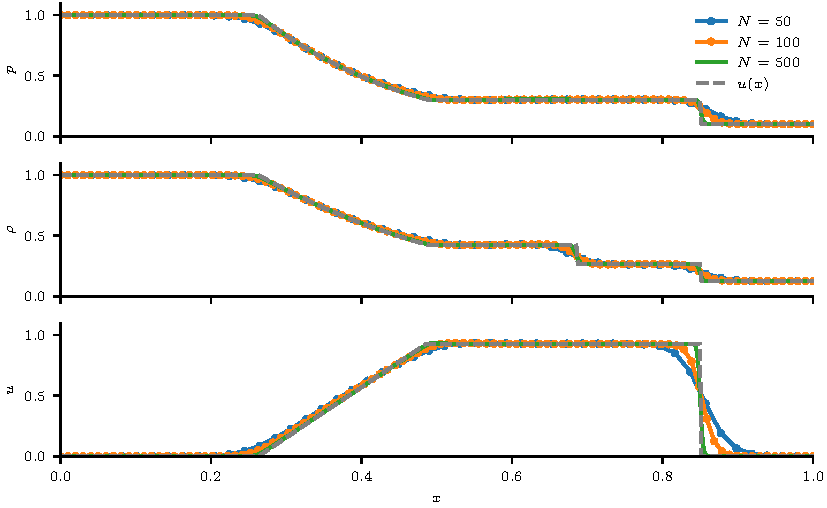
\includegraphics[width=1.0\linewidth]{resolution_study.pdf}
  \mycaption{Solutions to the Sod problem for various resolutions.}{The resolutions plotted are $N=50,\ 100,$ and $500$ (solid lines) and the analytical solution is also shown (dotted line). The solutions at resolutions $N=50$ and $N=100$ are shown with dots at the grid point locations. The solution given for $t=0.2$ and the shock viscosity parameters are $c_1 = 0.77$ and $c_2 = 0$.}
  \label{fig:resolution_study}
\end{figure}

\begin{figure}[t]
  \centering
  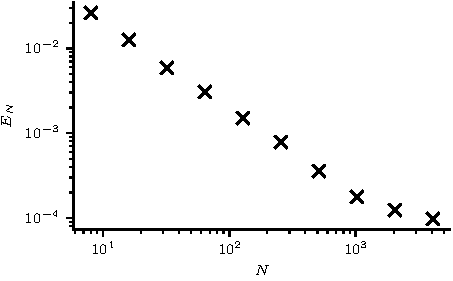
\includegraphics[width=0.5\linewidth]{effect_of_res_on_error.pdf}
  \mycaption{Numerical error as a function of resolution.}{Each data point represents a simulation run with the optimal shock parameter values to $t=0.2$ using a resolution $N$. The error is calculated via~\eqref{eq:total_error}.}%
  \label{fig:effect_of_res_on_error}
\end{figure}

The resolution affects the ability of the numerical scheme to adequately resolve discontinuities in the numerical solution. Figure~\ref{fig:resolution_study} shows three sample simulations at resolutions of $N=50$, $100$ and $500$. Although $N=500$ is a computationally cheap resolution for 1D simulations, $500$ grid points per dimension in 3D MHD is a typical resolution at current computational limits. This simulation gives an indication of how well a fully 3D scheme might cope with shocks. Even with a low resolution of $N=50$, no major features of the solution have been lost, although the discontinuities are artificially spread over a large distance.

Figure~\ref{fig:effect_of_res_on_error} shows the error $E_N$ as a function of resolution. The slope of the dependence suggests the global error is linearly dependent on the inverse of the resolution, instead of a quadratic dependence as expected from a second order scheme. This may be a result of the numerical scheme reverting to first order in the vicinity of discontinuities, or it may indicate an error in the code or the scheme. Again, since this is only an illustrative toy implementation of the numerical scheme, it is not worth delving into further.

\section{Conclusion}

This chapter presents a 1D, hydrodynamic code using the same numerical scheme as the 3D, MHD code Lare3d. The implementation of the scheme to the 1D, compressible Euler equations is described, along with the van Lee flux limiter and Wilkins shock viscosity, two techniques used to more effectively capture shocks. The way in which Lare3d extends the same scheme and shock capturing techniques is discussed. Finally, results of a numerical test of an implementation of the scheme are presented.

\chapter{The switching model}
\label{chp:switching_model}

\graphicspath{{images/development_of_switching_model/}}

In this chapter I initially explore the effect of resolution on the Braginskii model of viscosity, showing that a direct numerical implementation of the tensor~\eqref{eq:brag_new} fails to capture the transition between isotropic and anisotropic viscosity in the vicinity of magnetic null points, when such an implementation is used in simulations performed at resolutions typical of modern 3d simulations. This motivates the implementation of a different model of viscosity, the switching model, which approximates the Braginskii tensor as an interpolation between fully-isotropic and fully-parallel tensors. Three potential interpolation (or switching) functions are introduced: a phenomenological model derived from considering the probability of momentum transport in different magnetic field strengths, and two functions based on coefficients of the full Braginskii tensor. The development of the first function, referred to here as the von Mises switching function can be found in~\cite{mactaggartBraginskiiMagnetohydrodynamicsArbitrary2017}. Finally, I present the results of a suite of simulations performed at different resolutions which illustrate the differences between the models and are used to gauge their efficacy.

\section{The transition from isotropic to anisotropic in the full Braginskii tensor}

In strong magnetic fields, the Braginskii tensor can be approximated by the parallel term~\eqref{eq:braginskii_parallel_term} while in weak or null fields, the tensor reduces to that of isotropic viscosity~\eqref{eq:isotropic_viscous_tensor}. Between these extremes the perpendicular and drift components of the tensor can become relevant~\cite{erdelyiResonantAbsorptionAlfven1995a}. The form of the Braginskii tensor as written in equation~\eqref{eq:brag_new} is nearly in a form useful in understanding how quickly the tensor transitions from isotropic to anisotropic with changing magnetic field strength, since the isotropic component is completely isolated. Similarly, the parallel component can be isolated by further rewriting the tensor as,
\begin{equation}
\begin{split}
\ten{\sigma}_{\rm brag} &= \frac{3\eta_0+\eta_1-4\eta_2}{3}\ten{W}^{(0)}\\% \label{new1} \\
& + (\eta_2-\eta_1)[\ten{W}(\vec{b}\otimes\vec{b})+(\vec{b}\otimes\vec{b})\ten{W} - \frac{2}{3}(\ten{W}\vec{b}\cdot\vec{b})\ten{I}] \\%\label{new3}\\
& + \eta_1\ten{W},%\label{new4}
\end{split}
\label{eq:brag_new2}
\end{equation}

\begin{figure}[t]
  \centering
  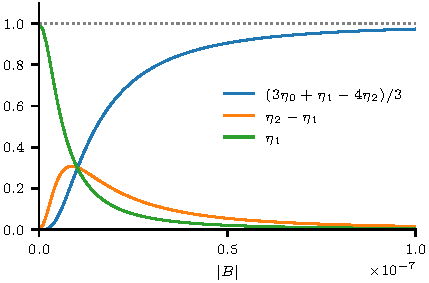
\includegraphics[width=0.5\linewidth]{brag_coeffs_2.pdf}
  \mycaption{Coefficients of the terms in the Braginskii tensor~\eqref{eq:brag_new2} normalised against $\eta_0$.}{In these plots, $\alpha = 10^{8}$, a value realistic of the corona.}%
  \label{fig:brag_coeffs2}
\end{figure}

Figure~\ref{fig:brag_coeffs2} presents the magnitudes of the coefficients of each of the terms in equation~\eqref{eq:brag_new2} when $\alpha = 10^{8}$ (recall that the coefficients $\eta_1$ and $\eta_2$ are defined in terms of the quantity $x=\alpha |\vec{B}|$). Over the extremely small range between $|\vec{B}| = 0$T and $10^{-7}$T, the Braginskii tensor goes from completely isotropic to nearly completely parallel. Over the same range the coefficient corresponding to the perpendicular viscosity becomes relatively significant before tending to zero for large $|\vec{B}|$. The small transition region presents a problem in the numerical simulation of anisotropic viscosity, where the magnetic field strength likely changes more rapidly in space than can be captured by the coefficients in equation~\eqref{eq:brag_new2}.

In the simulations of magnetic null points found later in section~\ref{sec:slow_null_point}, the magnetic field strength changes linearly in the $x$-direction. Given a typical grid spacing of $\Delta x = 0.01$, the jump in magnetic field from one grid point to the next is $5\times 10^{-5}$ T. This is much greater than the range over which the Braginskii tensor transitions between isotropic and anisotropic regimes and the viscous response is under-resolved as a result. For these simulations, the resolution would have to increase by a factor of $100$ per dimension to even begin to resolve the region of transition. Whether this region is physically significant or not is unknown, however, given the abundance of observable null points and their involvement in high-energy phenomena, it is possible that the isotropic (and perpendicular) viscosity near a null plays an important part in its dynamics. At the resolutions typically studied in general 3D MHD simulations (between $300$ and $1000$ grid points per dimension) the isotropic regions in the vicinity of null points are likely to be poorly resolved. This is particularly true in simulations where null points are not the main focus of the simulation, but are dynamically created by some process.

Computational solutions such as refining the mesh near the null or implementing a multigrid method may help to improve the resolution of a given simulation and better resolve the viscosity transition region, however such approaches can be complex to implement in existing codes. An alternative to improving the resolution itself is to artificially scale $|\vec{B}|$ in the expression for the parallel Braginskii transport parameter~\eqref{eq:perp_visc_coeff} in order to enlarge the isotropic region to resolvable scales. This is done by modifying the arguments of the parallel and perpendicular coefficients in~\eqref{eq:perp_visc_coeff} and~\eqref{eq:drift_visc_coeff}. Equations~\eqref{eq:perp_visc_coeff} and~\eqref{eq:drift_visc_coeff} are written in terms of the dimensionless quantity $x = \alpha |\vec{B}|$, where $\alpha$ is a physical parameter given by the expression $\alpha = e \tau / m$. By artificially setting $\alpha$ to a value other than its physical value, the viscous response can be adapted to a given resolution.

Consider the effect of decreasing $\alpha$ on the coefficients shown in Figure~\ref{fig:brag_coeffs2}. Decreasing $\alpha$ exaggerates the size of the region near $|\vec{B}| = 0$ where the isotropic and perpendicular components are significant. In this way, $\alpha$ can be used as a controllable parameter to prescribe the size of the region of isotropic (or perpendicular) viscosity around a null point.

As well as exaggerating the region of isotropic viscosity, this approach requires exaggerating the region of perpendicular viscosity. To see this, consider the contributions to the field-aligned component of~\eqref{eq:brag_new2} in a coordinate system where the field lies in the $z$-direction,
\begin{equation}
  \label{eq:z_aligned_field}
(\sigma_{brag})_{zz} = \frac{3\eta_0+\eta_1-4\eta_2}{3} W_{zz} + (\eta_2 - \eta_1) \frac{4}{3} W_{zz} + \eta_1 W_{zz} = \eta_0 W_{zz}.
\end{equation}
If the coefficient of the perpendicular component $\eta_2 - \eta_1$ is not scaled identically to the isotropic and parallel coefficients, the terms in~\eqref{eq:z_aligned_field} no longer cancel appropriately and the field-aligned momentum transport is no longer independent of $|\vec{B}|$. Hence, scaling the coefficients in the Braginskii tensor to enlarge the isotropic region necessarily requires also scaling the size of the perpendicular region. While this may be a useful feature, creating a purely parallel-isotropic switching model offers an alternative which avoids the inclusion of perpendicular viscosity altogether.

\section{The switching model}

The switching model is a model of viscosity that approximates the full Braginskii tensor throughout most of the solar corona. By stripping out the perpendicular and drift components of the full Braginskii tensor, the switching model presents a cleaner, better-resolved model of viscosity. It focuses on what are, in many cases, the most physically important parts of anisotropic viscosity in the solar corona: the parallel and isotropic components. The idea at the core of the model is the interpolation between the parallel and isotropic tensors, mirroring the way in which the Braginskii tensor changes in strong and weak fields.

For a general interpolation function $\tilde{s}(|\vec{B}|)$, henceforth referred to as a switching function, the switching model takes the form,
\begin{equation}
  \label{eq:switching_model_simple}
\ten{\sigma}_{\text{swi}} = \eta_0 \left( 1 - \tilde{s} \right) \ten{W} + \eta_0 \tilde{s} \ten{W}^{(0)},
\end{equation}
or
\begin{equation}
  \label{eq:switching_model}
\ten{\sigma}_{\text{swi}} = \eta_0 \left( 1 - \tilde{s} \right) \ten{W} + \eta_0 \tilde{s} \left[\frac{3}{2}(\ten{W}\vec{b}\cdot\vec{b}) \left( \vec{b} \otimes \vec{b} - \frac{1}{3}\ten{I} \right)\right].
\end{equation}
This trivially satisfies the requirement that the field-aligned component of momentum transport is independent of $|\vec{B}|$. The switching function may be thought of as a measure of the degree of anisotropy in the momentum transport, dependent on the local magnetic field strength, where $\tilde{s}(|\vec{B}|) = 0$ corresponds to totally isotropic and $\tilde{s}(|\vec{B}|) = 1$ corresponds to totally anisotropic.

\subsection{The von Mises switching function}

\label{sec:switching_function}

\begin{figure}[t]
  \centering
  \includegraphics[width=0.5\linewidth]{s_against_a.pdf}
  \mycaption{The von Mises switching function $s$, $s^2$ and the spline representation of $s^2$ as functions of $a$.}{}%
  \label{fig:s_against_a}
\end{figure}

The von Mises switching function was originally developed by MacTaggart and Vergori\footnote{While I am cited as an author in the referenced paper, I became involved in the research after the switching model itself was developed. My contribution is in the numerical implementation of the model and the development and analysis of the simulations.}~\cite{mactaggartBraginskiiMagnetohydrodynamicsArbitrary2017}. In this model, a measure of anisotropy is developed by considering the direction of momentum transport to be governed by a particular orientation probability distribution, where a greater field strength increases the probability of the momentum transport aligning with the field. Choosing the von Mises distribution leads to the form $\tilde{s} = s^2$ where
\begin{equation}
  \label{eq:switching_function}
s(|\vec{B}|) = \frac{3 \exp[2a]}{2\sqrt{2\pi a} \text{erfi}[\sqrt{2a}]} - \frac{1}{2}\left[ 1 + \frac{3}{4a} \right],
\end{equation}
and $a(|\vec{B}|)$ is a constitutive function controlling the sensitivity of the interpolation function to changes in magnetic field strength. Here, erfi is the imaginary error function. Where this model is used in throughout this thesis, the choice $a(|\vec{B}|) = a_0 |\vec{B}|^2$ is made, where $a_0$ is a parameter which effectively controls the size of the isotropic region near magnetic null points. 

For more efficient evaluation of~\eqref{eq:switching_function}, it is approximated and implemented numerically using a piecewise polynomial spline. For $a < 0.5051$, the function is clamped to $s=0$ and for $a > 29.41$, $s=1$. Between these cut-offs, $s^2$ is approximated using eight splines. The upper cut-off gives the halo effect in the results presented later in section~\ref{sec:slow_null_point}. The function~\eqref{eq:switching_function}, its square and its spline approximation are plotted in Figure~\ref{fig:s_against_a}. 

\subsection{Braginskii-inspired switching functions}

Two alternatives to the phenomenological von Mises switching function~\eqref{eq:switching_function} can be extracted from the Braginskii tensor itself. The tensor, written in the form~\eqref{eq:brag_new2}, suggests two alternative interpolation functions, one based on the coefficient for the isotropic part $\eta_1$, and another based on the coefficient of the parallel part $(3\eta_0+\eta_1-4\eta_2)/3$. Figure~\ref{fig:brag_coeffs2} shows that the coefficient of the perpendicular term $\eta_2 - \eta_1$ is not suitable as an interpolation function.

The Braginskii switching functions are easiest written using a form of $\eta_2(x)$ (equation~\eqref{eq:perp_visc_coeff}) normalised against $\eta_0$,
\begin{equation}
  \label{eq:eta_function}
  \tilde{\eta}(x) = \eta_2(x)/\eta_0 = \frac{\tfrac{6}{5}x^2 + 2.23}{2.23 + 4.03 x^2 + x^4}.
\end{equation}
This allows us to define a new interpolation function based on the coefficient of the parallel part of the Braginskii tensor as
\begin{equation}
  \label{eq:alt_switching1}
s_{par}(x) = \frac{3+\tilde{\eta}(2x)-4\tilde{\eta}(x)}{3},
\end{equation}
and another based on the coefficient of the isotropic part,
\begin{equation}
  \label{eq:alt_switching2}
s_{iso}(x) = 1 - \tilde{\eta}(2x).
\end{equation}

\begin{figure}[t]
  \centering
  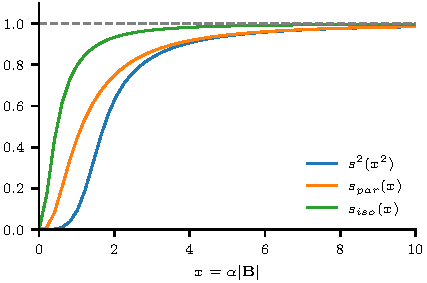
\includegraphics[width=0.5\linewidth]{alt_switching.pdf}
  \mycaption{Three potential switching functions.}{}%
  \label{fig:alt_switching}
\end{figure}

Figure~\ref{fig:alt_switching} plots the two Braginskii and the von Mises switching functions. The function $s_{par}$ shows the most similarity to the von Mises switching function, particularly the shallow slope near $|\vec{B}| = 0$, in contrast to the steeper slope of $s_{iso}$. Note that the argument of the von Mises switching function is the square of $x = \alpha |\vec{B}|$. This is a direct result of the choice of constitutive function $a(|\vec{B}|) = a_0 |\vec{B}|^2$, where $a_0 = \alpha^2$ for comparison.

\subsection{Calibrating the interpolation functions}

The parameters $a_0$ and $\alpha$ control the effective size of the isotropic region by controlling the degree to which the viscosity is anisotropic for a given field strength. From Figure~\ref{fig:alt_switching}, the viscosity can be considered anisotropic when $\alpha |\vec{B}| = 10$. If the viscosity should be considered anisotropic when the field strength is some reference value $B_0$ then $\alpha = 10/B_0$ gives the appropriate parameter choice. Similarly, for the von Mises function, $a_0 = 100/B_0^2$. This calibration  can be seen in practice in the following example.

In the numerical experiments performed in chapter~\ref{chp:null_point_khi}, the magnetic field strength increases linearly with distance from the null point and the grid separation is found to be $\Delta x \approx 0.014$. If we wish to consider the viscosity fully anisotropic at a radius of, say, ten grid points, the field at $x = 10 \Delta x$ is $|\vec{B}| = 0.14$, resulting in a calibrated $\alpha \approx 70$. The associated von Mises parameter would be $a_0 \approx 4900$. 

\section{Implementation of viscosity in Lare3D}

The two types of viscosity already present in the Lare3D code are shock and isotropic viscosities. Since shock viscosity is turned off for most numerical experiments presented in this thesis, I shall only detail the numerical implementation of isotropic viscosity, before discussing the implementations of the Braginskii and switching models.

\subsection{Review of the implementation of isotropic viscosity}

The isotropic viscous stress tensor is implemented in Lare3D as six 3D arrays, each storing the values for the six required components of a symmetric stress tensor. These are filled during the Lagrangian step using equation~\eqref{eq:isotropic_viscous_tensor}, where the components of the strain rate tensor are calculated via equation~\eqref{eq:rate_of_strain}. This stress tensor is used in the calculation of forces in the momentum equation and in the calculation of viscous heat contribution in the energy equation. This entire process is presented in detail below.

The strain rate tensor $\ten{W}$ is calculated in the code as \verb|s*|
\begin{verbatim}
sxx = (2.0_num * dvxdx - dvydy - dvzdz) * third
\end{verbatim}
for the diagonal elements \verb|sxx|, \verb|syy| and \verb|szz| and
\begin{verbatim}
sxy = dvxy * 0.5_num
\end{verbatim}
for the off-diagonal elements \verb|sxy|, \verb|sxz| and \verb|syz|. Since $\ten{W}$ is a symmetric tensor, only six components need to be calculated. The gradients of velocity, \verb|dv*|, are calculated using finite differences between appropriate velocity components, where the velocity is averaged over neighbouring grid points to ensure the resultant stress tensor is defined at the appropriate grid location. Note, the calculation of \verb|s*| in the code is a factor of a half smaller than the definition of $\ten{W}$ used in this thesis, equation~\eqref{eq:rate_of_strain}. This is corrected for during the calculation of the viscous stress tensor, stored in the variable \verb|q*|, where a factor of two is included,
\begin{verbatim}
qxx(ix,iy,iz) = qxx(ix,iy,iz) + 2.0_num * sxx * rho(ix,iy,iz) * visc3
\end{verbatim}
and similarly for the other five components of the tensor. The multiplication by \verb|rho| at this point is cancelled out at a later stage.

The gradient of the tensor is used in the calculation of the forces in the momentum equation in the following way. The tensor values must be averaged to ensure the resultant gradient is correctly aligned with the velocity grid locations. Similar calculations are carried out for the other components of the stress tensor and force vector. This same code is used to include the anisotropic viscous stress tensors when they are enabled.
\begin{verbatim}
w1 = (qxx(ix ,iy ,iz ) + qxx(ix ,iyp,iz ) &
    + qxx(ix ,iy ,izp) + qxx(ix ,iyp,izp)) * 0.25_num
w2 = (qxx(ixp,iy ,iz ) + qxx(ixp,iyp,iz ) &
    + qxx(ixp,iy ,izp) + qxx(ixp,iyp,izp)) * 0.25_num
fx = fx + (w2 - w1) / dxc(ix)
\end{verbatim}

The viscous heat is calculated using
\begin{verbatim}
visc_heat(ix,iy,iz) = &
      qxy(ix,iy,iz) * dvxy  + qxz(ix,iy,iz) * dvxz &
    + qyz(ix,iy,iz) * dvyz  + qxx(ix,iy,iz) * dvxdx &
    + qyy(ix,iy,iz) * dvydy + qzz(ix,iy,iz) * dvzdz
\end{verbatim}
and, just as in the calculation of the forces above, this same code is used to calculate the viscous heat generated by the anisotropic viscous tensors when they are enabled.

\subsection{Implementation of the Braginskii tensor}

Since the contribution of a generic viscous stress tensor to the momentum and energy equations is already included in the numerical implementation of isotropic viscosity, the only new piece of code required to implement a new stress tensor is the calculation of the stress tensor itself. The Braginskii tensor given by equation~\eqref{eq:brag_new} is implemented in the following way and, when enabled, replaces the calculation of the isotropic viscous stress tensor. 

The four coefficients of the terms in equation~\eqref{eq:brag_new} are calculated as
\begin{verbatim}
a = (3._num*visc3 + brag_visc1 - 4._num*brag_visc2)&
    / MAX(2._num*mB2**2, none_zero)
b = (brag_visc1 - visc3)/(2._num*mB2)
c = (brag_visc2 - brag_visc1)/(mB2)
d = brag_visc1
\end{verbatim}
where \verb|visc3| is the variable holding the value of $\eta_0$, \verb|brag_visc1| and \verb|brag_visc2| hold the values of $\eta_1$ and $\eta_2$, calculated via equation~\eqref{eq:perp_visc_coeff}, and \verb|mB2| holds the value of $|\vec{B}|^2$. This calculation is performed in the following way
\begin{verbatim}
xi2 = (brag_alpha**2) * mB2
brag_visc_coeff = visc3*(6._num/5._num*xi2 + 2.23_num)&
                  / (2.23_num + 4.03_num*xi2 + xi2**2)
\end{verbatim}
where \verb|brag_alpha| is the parameter $\alpha$.

The quantity $(\ten{W} \vec{B}) \cdot \vec{B}$ and the tensor components of $\vec{B} \otimes \vec{B}$ are calculated using the following snippet.
\begin{verbatim}
calc_wbdotb = 2._num*(&
  (bx*sxx + by*sxy + bz*sxz)*bx &
+ (bx*sxy + by*syy + bz*syz)*by &
+ (bx*sxz + by*syz + bz*szz)*bz)

btxx = bx**2
btyy = by**2
btzz = bz**2
btxy = bx*by
btxz = bx*bz
btyz = by*bz
\end{verbatim}

This allows the Braginskii stress tensor to be calculated using
\begin{verbatim}
bsxx = wbdotb*(a*btxx + b) + 2._num*d*sxx &
  + 4._num*c*(btxx*sxx + btxy*sxy + btxz*sxz)
\end{verbatim}
and similar for the diagonal \verb|bsxx|, \verb|bsyy| and \verb|bszz| components. The off-diagonal components are calculated using the following snippet.
\begin{verbatim}
bsxy = wbdotb*a*btxy + 2._num*d*sxy &
  + 2._num*c*(btxx* sxy + btxy* syy + btxz* syz &
            +  sxx*btxy +  sxy*btyy +  sxz*btyz)
\end{verbatim}

Finally, the contribution from the Braginskii stress tensor is added to the total stress tensor using 
\begin{verbatim}
qxx = qxx + rho*bsxx
\end{verbatim}
and similar for the other components. A later calculation in Lare3D requires that the Braginskii stress tensor is multiplied by \verb|rho|.

\subsection{Implementation of the switching model}

The numerical implementation of the switching model is similar to the implementation of the Braginskii model detailed previously, with the exception of the tensor itself which is calculated using
\begin{verbatim}
bsxx = visc3*((1.0_num-s2)*sxx*2.0_num + 1.5_num*s2&
/MAX(mB2**2, none_zero)*wbdotb*(btxx - mB2*third))
\end{verbatim}
where \verb|s2| holds the local value of the chosen switching function, and the diagonal \verb|bsxx|, \verb|bsyy| and \verb|bszz| components are calculated similarly. The off-diagonal components are calculated using the following snippet.
\begin{verbatim}
bsxy = visc3*((1.0_num-s2)*sxy*2.0_num + 1.5_num*s2&
/MAX(mB2**2, none_zero)*wbdotb*(btxy))
\end{verbatim}

As discussed in section~\ref{sec:switching_function}, the von Mises switching function $s^2$ is implemented as a spline approximation. The Braginskii switching functions~\eqref{eq:alt_switching1} and~\eqref{eq:alt_switching2} have been simplified using the Python package \emph{SymPy} and are implemented directly. 

\section{Application to stressed null point}

\label{sec:slow_null_point}

As a test of the switching model in a non-trivial topology, a series of simulations of magnetic null points subjected to twisting motions were carried out. Isotropic, full Braginskii and switching viscosity, with the three switching functions presented here, were used and the results compared.

\subsection{Numerical setup}

The non-dimensionalised MHD equations are solved using the code Lare3d, described in chapter~\ref{chp:numerical_methods}. For the purposes of testing and comparing the various models, the typical values used to non-dimensionalise the MHD equations are arbitrary\footnote{For reference, the typical values are $B_0 = 0.03$T, $L_0 = 180\times10^{3}$m and $\rho_0 = 1.67\times10^{-4}$kgm$^{-3}$, for the magnetic field strength, length and density, respectively.}. The domain is a cube of dimension $[-3, 3]^3$ and the resolution is $500$ grid points per dimension. The magnetic field is initially prescribed as a linear magnetic null point,
\begin{equation}
  \label{eq:null_mag_field}
\vec{B} = (x, y, -2z)^T.
\end{equation}
The density $\rho$ is initially set to unity, the velocity to $\vec{u} = \vec{0}$, and the internal energy initially $\varepsilon = \gamma-1$, where $\gamma = 5/3$ is the specific heat ratio.

On the lower boundary ($z=-3$) the velocity takes the form of a twisting vortex
\begin{equation}\label{ramp}
\boldsymbol{u} = \frac{v_0}{2}\left[1+\tanh\left(2\frac{t-t_0}{t_d}\right)\right]\boldsymbol{u}_h,
\end{equation}
with $\boldsymbol{u}_h = (u_x',u_y',0)^{\rm T}$ and
\begin{equation}\label{vprime}
u_x' = \left\{\begin{array}{cc}
-\pi y\displaystyle\frac{\sin(\pi r)}{r} &\quad{\rm if}\quad r^2<1, \\[8pt]
\displaystyle 0 &\quad{\rm if}\quad r^2 \ge 1,
\end{array}\right. \quad
u_y' = \left\{\begin{array}{cc}
\pi x\displaystyle\frac{\sin(\pi r)}{r} &\quad{\rm if}\quad r^2<1, \\[8pt]
\displaystyle 0 &\quad{\rm if}\quad r^2 \ge 1,
\end{array}\right.
\end{equation}
where $r^2=x^2+y^2$. On the opposite boundary, the twisting motion is reversed. The maximum driving velocity is set to $v_0 = 0.05$. The acceleration parameters are set to $t_0 = 2$, the time at which the velocity is half its maximum, and $t_d = 1$, resulting in maximum velocity being achieved around $t\approx4$. On the boundaries, all other variables keep their initial values and the derivatives through each boundary is zero.

For comparison between the switching models, the switching parameters are set to $\alpha = 6$ and $a_0 = \alpha^2 = 36$. This dramatically exaggerates the size of the isotropic region around the null point and allows good comparison of the viscosity models.

\subsection{Results}

\label{sec:slow_null_results}

The primary difference between isotropic and both anisotropic viscosity models is the magnitude and spatial distribution of the viscous heating. Isotropic viscosity overestimates the total heat generated by several orders of magnitude, when compared to any anisotropic model. The switching models all share some characteristics with the Braginskii model and each present different advantages.

\subsubsection{Differences in viscous heating rates}

\begin{table}[t]
  \centering
  \caption{Total heat generated up to $t=10$ by each model of viscosity.}
  \label{tab:total_heating_slow_null}
  \begin{tabular}{ccccc}
Iso & Brag & Swi (von Mises) & Swi (par) & Swi (iso)\\
\midrule
$4.04 \times 10^{-3}$ & $5.25 \times 10^{-5}$ & $6.81 \times 10^{-5}$ & $7.80 \times 10^{-5}$ & $4.39 \times 10^{-5}$
\end{tabular}
\end{table}

Table~\ref{tab:total_heating_slow_null} shows the total heat generated by $t=10$ for each viscosity model. The isotropic model overestimates the viscous heating by approximately two orders of magnitude compared to any of the anisotropic models. The switching models all dissipate similar amounts of heat to the Braginskii model, indicating that these models are approximating well the Braginskii tensor. The variance between each of the anisotropic models can be explained by considering how the isotropic and anisotropic parts of the tensors each contribute to the heating profile.

\begin{figure}[t]
    \centering
    \hfill
    \begin{subfigure}{0.32\textwidth}
      \includegraphics[width=1.0\linewidth]{iso_heating_iso_10.pdf}
      \caption{Isotropic}%
      \label{fig:iso_heating_iso_10}
    \end{subfigure}
    \hfill
    \begin{subfigure}{0.32\textwidth}
      \includegraphics[width=1.0\linewidth]{iso_heating_brag_10.pdf}
      \caption{Braginskii}%
      \label{fig:iso_heating_brag_10}
    \end{subfigure}
    \hfill
    \begin{subfigure}{0.32\textwidth}
      \includegraphics[width=1.0\linewidth]{iso_heating_switching_10.pdf}
      \caption{Switching (von Mises)}%
      \label{fig:iso_heating_switching_10}
    \end{subfigure}
    \begin{subfigure}{0.32\textwidth}
      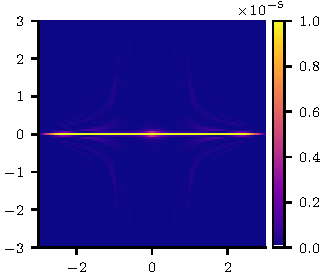
\includegraphics[width=1.0\linewidth]{iso_heating_switching2_10.pdf}
      \caption{Switching (par)}%
      \label{fig:iso_heating_switching2_10}
    \end{subfigure}
    \begin{subfigure}{0.32\textwidth}
      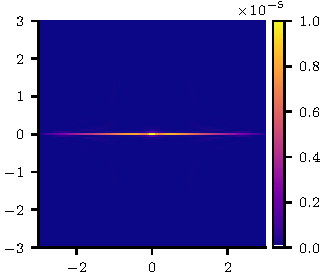
\includegraphics[width=1.0\linewidth]{iso_heating_switching3_10.pdf}
      \caption{Switching (iso)}%
      \label{fig:iso_heating_switching3_10}
    \end{subfigure}

    \mycaption{Isotropic heating generated by the viscosity models.}{Shown are plots of the isotropic heating produced by the isotropic, full Braginskii and switching models at $t=10$, sliced through $y=0$. Note the peak colour of the isotropic plot is an order of magnitude greater than that of the anisotropic models.}
\label{fig:isotropic_heating}%
\end{figure}

Figure~\ref{fig:isotropic_heating} shows the isotropic heating rate at time $t=10$ for each viscosity model. Isotropic viscosity heats at a generally greater rate than the anisotropic models, and the heating is distributed more extensively throughout the null. The boundary of the numerical cut-off, where isotropic viscosity turns off in the von Mises switching model, can be seen in figure~\ref{fig:iso_heating_switching_10}. The isotropic heating generated by the two Braginskii-inspired models show most similarity to that of the Braginskii model, with the isotropic-based switching model showing a nearly identical heating profile. This is to be expected since the coefficients of the isotropic contributions to the Braginskii and isotropic-based switching tensors are identical. The relative magnitude of the isotropic heating contributions for each anisotropic model reflects the total heat generated in table~\ref{tab:total_heating_slow_null}, showing that the isotropic model overestimates viscous heating by two orders of magnitude.


Figure~\ref{fig:anisotropic_heating} shows the contributions to viscous heating from the anisotropic parts of the Braginskii and switching tensors. The anisotropic heating generated by the Braginskii tensor is dominated by the perpendicular contribution near the fan plane. This again reveals the potential issue with artificially increasing $\alpha$, that alongside increasing the size of the isotropic region, the extent of the perpendicular contributions are similarly enhanced.

\subsubsection{The effect of resolution on the size of the isotropic region}

\begin{table}[t]
  \centering
  \caption{Total heat generated up to $t=10$ by each model of viscosity for resolutions of $N=100$ and $500$.}
  \label{tab:slow_null_results_resolution}
  \begin{tabular}{c|cccc}
Model &  Brag & Swi (von Mises) & Swi (par) & Swi (iso)\\
\midrule
$N=100$ &  $5.74 \times 10^{-5}$ & $7.13 \times 10^{-5}$ & $8.39 \times 10^{-5}$ & $4.66 \times 10^{-5}$\\
$N=500$   & $5.25 \times 10^{-5}$ & $6.81 \times 10^{-5}$ & $7.80 \times 10^{-5}$ & $4.39 \times 10^{-5}$  \end{tabular}
\end{table}

Identical simulations were run to those described in~\ref{sec:slow_null_results} but with the resolution reduced to $N=100$ per dimension. This allows a clear demonstration of the effect of poor resolution on anisotropic heating near the null point itself. While table~\ref{tab:slow_null_results_resolution} shows the global estimate of total viscous heat remains consistent across viscosity models, figure~\ref{fig:anisotropic_heating} shows the spatial distribution of the heating does not.

Figure~\ref{fig:anisotropy_bleeding} shows the heating rate produced by the anisotropic parts of the Braginskii and switching models and reveals the primary issue with the Braginskii model. When the resolution is too low to properly resolve the region around the null point, the Braginskii model erroneously heats anisotropically, primarily due to the artificially increased $\alpha$ enhancing the perpendicular components near the null point. This issue is mitigated by the switching models, all of which remove the perpendicular components of the Braginskii tensor. At the higher resolution of $N=500$ the von Mises switching model appears to remove more anisotropic heating than may be necessary however this could be solved by optimising the parameter $a_0$. Both Braginskii-based switching models show greater similarity to the Braginskii model without suffering from the issue of anisotropy at the null. Away from the null all switching models give similar results to the Braginskii model.

\section{Model efficiency}

In order to evaluate the real efficiency of each model of viscosity, a set of benchmark tests were run with the same physical setup as that of the test simulations found in section~\ref{sec:slow_null_point}, although changing the initial or boundary conditions should not affect the results. The resolution is set to $N=100$, all output is disabled, only one CPU core is used, and the simulations run for only $100$ timesteps. This number of timesteps allows the main loop of the simulation to run for a longer time than the overhead required to start and end the simulation, giving a more accurate estimate of the running time. The combination of the resolution and the number of timesteps results in the viscosity routines running $10^{8}$ times per simulation. The time is calculated via the linux \verb|time| command which reports millisecond accuracy. Due to other software running on the same machine, the total time can vary. To measure a more accurate running time, the test for each model is repeated $25$ times and the results averaged. The machine used to run these tests is a Dell all-in-one with a 4 core, Intel i7-6700 CPU running at 3.4 GHz and 16 GB of RAM. 

\begin{figure}[t]
  \centering
  \includegraphics[width=0.5\linewidth]{benchmark.pdf}
  \mycaption{Relative computational efficiency of viscosity models measured via mean runtime.}{The runtime for each viscosity model is scaled by the runtime for the isotropic model.}%
  \label{fig:benchmark}
\end{figure}

Figure~\ref{fig:benchmark} shows the average runtime for each model. Since the isotropic model requires only the calculation of the rate of strain tensor, it is the quickest. The Braginskii model, being the most complex, requires many additional calculations to be carried out and this is reflected in its poorer runtime. The switching models show similar efficiencies, worse than the isotropic model but mostly better than the Braginskii model, as expected from considering the number of required calculations. The differences between the runtimes of the different interpolation functions are slight, although the von Mises implementation appears moderately faster. This is likely due to the spline representation of the von Mises function requiring only one computation of a cubic, while the other switching functions require two.

\section{Conclusion}

This chapter details the switching model, a new model of anisotropic viscosity specifically designed for use in numerical simulations of the solar corona. The model offers an alternative to the Braginskii model, capturing the main physics while avoiding the problem of anisotropic heating at the null point itself. It does this by artificially enlarging the isotropic region surrounding magnetic null points. The switching model does this by exposing a tunable interpolation function which measures the degree of anisotropy (dependent on the local magnetic field strength) and interpolates between isotropic and fully field-aligned viscosity. Three candidate interpolation functions are presented and their efficacy and computational efficiency compared. The switching model is generally found to be computationally more efficient than the Braginskii model and offers a good approximation to it.

Overall, the three switching functions behave similarly and each provide unique advantages. While the von Mises switching function is computationally faster than the Braginskii-inspired functions, it is a phenomenological model and requires a spline approximation for efficient implementation. In contrast, the Braginskii switching functions utilise the interpolation already implicit in the Braginskii tensor and can be implemented directly in the code. 

In chapters~\ref{chp:kink_instability} and~\ref{chp:kink_instability_straight} the von Mises switching model is employed although the field is strong enough everywhere that the tensor reduces to purely parallel (i.e. $\tilde{s} = 1$ everywhere). In chapter~\ref{chp:null_point_khi} the Braginskii-inspired parallel function~\eqref{eq:alt_switching1} is used to avoid the numerical cut-off associated with the spline representation.

\begin{figure}[t]
    \hfill
    \begin{subfigure}{0.49\textwidth}
      \includegraphics[width=1.0\linewidth]{aniso_heating_brag_10.pdf}
      \caption{Braginskii}%
      \label{fig:aniso_heating_brag_10}
    \end{subfigure}
    \hfill
    \begin{subfigure}{0.49\textwidth}
      \includegraphics[width=1.0\linewidth]{aniso_heating_switching_10.pdf}
      \caption{Switching (von Mises)}%
      \label{fig:aniso_heating_switching_10}
    \end{subfigure}
    \hfill
    \begin{subfigure}{0.49\textwidth}
      \includegraphics[width=1.0\linewidth]{aniso_heating_switching2_10.pdf}
      \caption{Switching (par)}%
      \label{fig:aniso_heating_switching2_10}
    \end{subfigure}
    \hfill
    \begin{subfigure}{0.49\textwidth}
      \includegraphics[width=1.0\linewidth]{aniso_heating_switching3_10.pdf}
      \caption{Switching (iso)}%
      \label{fig:aniso_heating_switching3_10}
    \end{subfigure}
    \mycaption{Anisotropic heating generated by the full Braginskii and switching models at time $t=10$.}{Close to the fan plane the Braginskii model shows notably greater anisotropic heating than any of the switching models. The switching models all appear similar though with minor differences near the null point.}
\label{fig:anisotropic_heating}%
\end{figure}

\begin{figure}[t]
    \hfill
    \begin{subfigure}{0.49\textwidth}
      \centering
      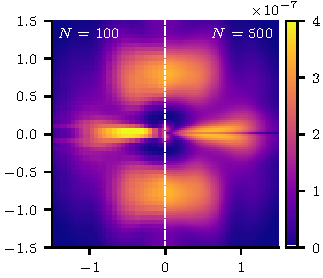
\includegraphics[width=1.0\linewidth]{diff_brag_resolution.pdf}
      \caption{Braginskii}%
      \label{fig:diff_brag_resolution}
    \end{subfigure}
    \hfill
    \begin{subfigure}{0.49\textwidth}
      \includegraphics[width=1.0\linewidth]{diff_switching_resolution.pdf}
      \caption{Switching (von Mises)}%
      \label{fig:diff_switching_resolution}
    \end{subfigure}
    \hfill
    \begin{subfigure}{0.49\textwidth}
      \includegraphics[width=1.0\linewidth]{diff_switching2_resolution.pdf}
      \caption{Switching (par)}%
      \label{fig:diff_switching2_resolution}
    \end{subfigure}
    \hfill
    \begin{subfigure}{0.49\textwidth}
      \includegraphics[width=1.0\linewidth]{diff_switching3_resolution.pdf}
      \caption{Switching (iso)}%
      \label{fig:diff_switching3_resolution}
    \end{subfigure}

    \mycaption{The effect of resolution on anisotropic heating rates.}{The anisotropic heating rate is plotted at resolutions of $100$ (left of each plot) and $500$ (right of each plot) grid points per dimension and both plots are slices through $x=0$ at $t=5$. When the null point is less resolved (left half of both figures) Braginskii viscosity erroneously permits anisotropic heating at the null. At higher resolutions (left half of both figures) the null is better resolved and much less anisotropic viscous heating is found at the null. All switching models avoid this issue.}
\label{fig:anisotropy_bleeding}%
\end{figure}

\chapter{Application to the kink instability}
\label{chp:kink_instability}

\graphicspath{{images/kink_instability/}}

\section{Introduction}
\label{sec:kink_introduction}

In this chapter I investigate the effects of anisotropic viscosity on the kink instability~\cite{hoodKinkInstabilitySolar1979, hoodCoronalHeatingMagnetic2009}, believed to be a trigger for flares~\cite{srivastavaObservationKinkInstability2010} and an important mechanism in the theory of coronal heating through nanoflares~\cite{browningHeatingCoronaNanoflares2008a}. The instability has also been studied using shock viscosity~\cite{hoodCoronalHeatingMagnetic2009,barefordShockHeatingNumerical2015} but a detailed investigation of the effects of Newtonian and Braginskii viscosity has not, to the best of my knowledge, been performed. In particular, the main aim of this investigation is to provide insight into the effect of the choice of viscosity model on the nonlinear dynamics and relaxation of a twisted coronal loop, where the kink instability converts magnetic energy to heat through Ohmic heating generated via current structures and through viscous heating generated via flow structures. I aim to give an estimate of how well viscous heating (using both isotropic and anisotropic models) performs when compared with Ohmic heating. This study extends previous work~\cite{hoodCoronalHeatingMagnetic2009} which also considers the kink instability in a zero-current loop (details given below). However, in contrast to~\cite{hoodCoronalHeatingMagnetic2009}, only background resistivity and viscosity are used as the two mechanisms of heat generation (that is, shock viscosity and anomalous resistivity are disabled). This investigation also provides further validation of the switching model in a simpler topology to that used by MacTaggart et al.~\cite{mactaggartBraginskiiMagnetohydrodynamicsArbitrary2017}, simpler in that there are no null points present in the field at any time.

The layout of the chapter is as follows. The coronal loop model is described in Section~\ref{sec:model-setup}. Details of the numerical setup and methods used in the analysis of the simulation results are presented in Section~\ref{sec:general-numerical-setup}. Detailed numerical results of a typical case of a kink instability are given in Section~\ref{sec:results} with a particular focus on how the different viscosity models affect its nonlinear evolution. The results of the typical case are confirmed and generalised by a parameter study in Section~\ref{sec:results2} where the dependences of the Ohmic and the viscous heating on the resistivity and the dynamic viscosity are explored. Conclusions are summarised in Section~\ref{sec:conclusions}.

This chapter is an adaptation of a previously published paper~\cite{quinnEffectAnisotropicViscosity2020a}. 

\section{Coronal loop model}
\label{sec:model-setup}

A twisted magnetic flux rope is used as the model of an idealised coronal loop. The domain is a Cartesian box of dimension $[-2\text{ Mm},2\text{ Mm}] \times [-2\text{ Mm},2\text{ Mm}] \times [-10\text{ Mm},10\text{ Mm}]$ in the $x$, $y$ and $z$-directions, respectively. The state of the plasma is typical of the corona, with density $\rho$ initially $1.67\times 10^{-12} \text{ kg m}^{-3}$, and with plasma pressure $p$ such that the temperature of the plasma $T$ is initially $2\times10^{4} \text{ K}$ everywhere in the domain. The magnetic field $\vec{B}$ is constructed so that it is initially force-free and with zero axial current, line-tied at the boundaries, and twisted such that it is linearly unstable to the ideal kink instability. This configuration allows direct comparison to previous studies that use similar magnetic field configurations~\cite{hoodCoronalHeatingMagnetic2009,barefordShockHeatingNumerical2015,bothaObservationalSignaturesCoronal2012}. The field outside the flux tube is straight and has a strength of $5\times10^{-3} \text{ T}$. Given this temperature and magnetic field strength, the plasma beta is initially $\beta \approx 10^{-5}$, a value realistic for the corona. The evolution of this flux tube is governed by the nonlinear MHD equations described in section~\ref{sec:mhd_equations}.

\begin{table}[t]
\centering
\begin{tabular}{ccc|ccc}
$B_0$ & $L_0$ & $\rho_0$ & $u_A = B_0 / \sqrt{\rho_0 \mu_0}$ & $t_A = L_0/u_A$ & $T_0$ \\ \midrule
$5 \times 10^{-3} \ \text{T}$ & $1\ \text{Mm}$ & $1.67 \times 10^{-12} \ \text{kgm}^{-3}$ & $3.45\ \text{Mms}^{-1}$ & $0.29\ \text{s}$ & $1.73 \times 10^{9}K$\\
\end{tabular}
\caption{Reference values for the magnetic field, length, density, and
  temperature. These are used to non-dimensionalise the MHD
  equations \eqref{eq:mhda}--\eqref{eq:energy} and to calculate the reference values for velocity, time and temperature.}
\label{tab:reference-values}
\end{table}

The magnetic field is considered force-free, that is the field is constructed such that the Lorentz force is zero, or $(\nabla \times \vec{B})\times \vec{B} = 0$. In cylindrical coordinates $(r,\theta,z)$, the chosen force-free magnetic field takes the form $\nabla \times \vec{B} = \alpha(r)\vec{B}$, where $\alpha(r)$ is a function of a particular form that ensures the total axial current is zero. Aligning with previous work by Hood et al.~\cite{hoodCoronalHeatingMagnetic2009}, the smooth $\alpha(r)$ profile given as Case 3 in~\cite{hoodCoronalHeatingMagnetic2009} is used. Using this profile, the equilibrium magnetic field $\vec{B}$ is written as 
\begin{equation}
\begin{aligned}
  \label{eq:field-profile-r-lt-1}
  B_{\theta} &= \lambda r {(1 - r^2)}^3,\\
  B_z &= \sqrt{1 - \frac{\lambda^2}{7} + \frac{\lambda^2}{7}{(1 - r^2)}^7 - \lambda^2 r^2 {(1-r^2)}^6},\\
  \alpha(r) &= \frac{2 \lambda {(1-r^2)}^2 {(1-4r^2)}}{B_z},
\end{aligned}
\end{equation}
for $r \leq 1$ and
\begin{equation}
\begin{aligned}
  \label{eq:field-profile-r-gt-1}
  B_{\theta} &= 0 \\
  B_z &= \sqrt{1 - \frac{\lambda^2}{7}}\\
  \alpha(r) &= 0 ,
\end{aligned}
\end{equation}
for $r > 1$, where $\lambda$ is a parameter measuring the twist in the tube. The radial field throughout the domain is set to $B_r = 0$. As is done in~\cite{hoodCoronalHeatingMagnetic2009}, $\lambda = 1.8$ to ensure the tube is unstable to the ideal kink instability. The equilibrium velocity for this magnetic field configuration is $\vec{u} = \vec{0}$.

\begin{figure}[t]
  \centering
  \begin{subfigure}[b]{0.48\textwidth}
  \begin{center}
    \begin{overpic}[width=\textwidth]{field_line_plots/cropped/v1e-4r5e-4.5-isotropic_0000_cropped.png}
      \put (50,5) {\small\textbf{(a)}}
    \end{overpic}
  \end{center}
  \end{subfigure}
  \begin{subfigure}[b]{0.48\textwidth}
  \begin{center}
    \begin{overpic}[width=\textwidth]{alpha_profile.pdf}
      \put (47,54) {\small\textbf{(b)}}
    \end{overpic}
  \end{center}
  \end{subfigure}
  \caption{\textit{The initial field configuration.} In \textbf{(a)} field lines are plotted corresponding to inner (red), outer (blue) and straight (yellow) regions of twist, with slices of $\alpha(r)$ shown at the footpoints. In the slices, red corresponds to $\alpha(r) > 0$, blue to $\alpha(r) < 0$ and white to $\alpha(r) = 0$. In \textbf{(b)} the profiles of $\alpha(r)$ and the field components $B_z$ and $B_{\theta}$ across the flux tube are plotted.}
\label{fig:field_configuration}
\end{figure}

The form of $\alpha(r)$ in equations~\eqref{eq:field-profile-r-lt-1} and~\eqref{eq:field-profile-r-gt-1} splits the profile of the flux tube into three twist regions, the inner region of positive twist ($r\le0.5$), the outer region of negative twist ($0.5<r<1$) and the straight-field region of zero twist ($r\ge1$) as shown in Figures~\ref{fig:field_configuration}(a) and (b). These figures also illustrate the equilibrium field. Since the inner region is more tightly twisted, this field configuration results in only the inner region becoming unstable to the kink instability, rather than the global instability seen in non-zero-current loops~\cite{hoodKinkInstabilitySolar1979}. The regions of twist are used later to define a measure of reconnection.

Although the initial temperature is prescribed as $T=2\times10^{4} \text{ K}$, the equations simulated by the code are written using internal energy, thus the temperature is converted to internal energy using the non-dimensional relation $\varepsilon = T/(1-\gamma)$. Hence, the initial non-dimensionalised density and internal energy are uniformly given by
\begin{equation}
  \rho = 1,\quad \varepsilon = 8.66 \times 10^{-4},
\end{equation}
and have been non-dimensionalised using the reference values found in Table~\ref{tab:reference-values}. The initial magnetic field and velocity are set to their equilibrium states, discussed above, with the addition of a small perturbation.

In order to make a meaningful comparison of the following results with those of~\cite{hoodCoronalHeatingMagnetic2009}, identical initial magnetic field and velocity perturbations are used, calculated via a linear stability analysis (in ideal MHD) applied to a similar flux tube that uses a constant, piecewise profile for $\alpha(r)$~\cite{vanderlindenCompleteCoronalLoop1999,browningSolarCoronalHeating2003c,browningHeatingCoronaNanoflares2008a}.

At the boundaries, the line-tied condition on the magnetic field is satisfied by ensuring the field is constant and equal to its initial values given by equations~\eqref{eq:field-profile-r-lt-1} and~\eqref{eq:field-profile-r-gt-1}. Similarly, on the boundaries the density, internal energy and velocity $\vec{u}$ are considered constant and equal to their initial values. To close the system, the fluxes of all variables through each of the boundaries are set to zero. That is, on the $x$-boundary,
\begin{equation}
  \frac{\partial \vec{B}}{\partial x} = \frac{\partial \vec{u}}{\partial x} = \vec{0}; \quad \frac{\partial \rho}{\partial x} = \frac{\partial \varepsilon}{\partial x} = 0 \quad \text{for } x=\pm 2,
\end{equation}
and similarly, the $y$ and $z$ derivatives are zero on the $y=\pm2$ and $z=\pm10$ boundaries, respectively.

Since there are no nulls created during the evolution of the kink instability, the field remains strong everywhere and the viscosity reverts to fully parallel. To ensure this, the switching model~\ref{eq:switching_model} is used with the von Mises switching function~\ref{eq:switching_function} where $a_0 = 150$. 

\section{Methods}
\label{sec:general-numerical-setup}

In this section the parameters of the numerical setup is presented, and various tools and quantities used in the proceeding analysis are described.

\subsection{Numerical setup}

The MHD equations~\eqref{eq:mhda}---\eqref{eq:energy} were solved numerically using the Lare3d code~\cite{arberStaggeredGridLagrangian2001}, previously described in chapter~\ref{chp:numerical_methods}. Shock viscosity was disabled in order to properly investigate the effect of different viscosity models. In order to compare results with those of Hood et al.~\cite{hoodCoronalHeatingMagnetic2009} numerical tests were performed using shock viscosity instead of either the switching or isotropic models. Using the default shock viscosity parameters present in the code, the behaviour closely mirrors that of isotropic viscosity with $\nu\approx 5\times10^{-4}$. When both switching and shock viscosity are enabled, the shock viscosity dominates and, again, the behaviour mirrors that of isotropic viscosity.

The simulations were run at a resolution of $350 \times 350 \times 700$, with the exception of the parameter studies, which were run at a slightly higher resolution of $400 \times 400 \times 800$. Since the switching viscosity only acts parallel to the magnetic field, in perpendicular directions numerical diffusion dominates. By running several simulations at resolutions of $250 \times 250 \times 500$ up to $500 \times 500 \times 1000$, it was found that the effect of resolution was negligibly small until around $t=150$, well after the nonlinear phase of the instability. After this time there were some quantitative differences in outputs for different resolutions. However, the qualitative behaviour, described later, does not strongly depend on the resolution.

The numerical diffusion present in the simulations (due to the finite difference scheme employed in Lare3d) is estimated as $\tilde{\nu} = \tilde{\eta} = \tilde{u}_x L_x/N_x^2$. Taking a typical velocity of $\tilde{u}_x = 1$, i.e.\ the Alfv\'en velocity; $N_x = 350$ as the number of grid-points in the $x$-direction; and $L_x = 4$ as the length in the $x$ direction, the numerical diffusion coefficient is estimated as $\tilde{\nu} = \tilde{\eta} \approx 10^{-5}$. This provides a theoretical lower bound on simulating a physical viscosity or resistivity. In practice, setting the physical resistivity lower than $\eta \approx 5\times10^{-5}$ results in behaviour that does not converge with increasing resolution. This gives a practical lower bound for diffusion coefficients of $\tilde{\nu} = \tilde{\eta} \approx 5 \times 10^{-5}$. Thus, all results presented use physical diffusion coefficients (either viscosity or resistivity) greater than this lower bound.

\subsection{Methods of analysis}

\subsubsection{Connectivity}

The mean change in field line connectivity $\Delta\Phi_c$ is used as a practical measure of reconnection rate. The connectivity of a given field line $\Phi_c$ is determined by comparing its start and end points. Any field line that begins at one location in one of the loop footpoints will map to a corresponding point in the opposite footpoint. Following field lines from their starting point at $z=-10$ to their end point at $z=10$, lines are labelled depending on the twist regions in which they start and end. Initially, the field lines within each distinct region map one-to-one to the same region. As the field reconnects radially during the instability, field lines begin to start and end in different twist zones. The rate of reconnection is estimated by tracking the number of field lines that have changed twist zones within a set time period. This also serves as a visual representation of where such reconnection is occurring. It should be noted that this measure of reconnection does not take into account azimuthal reconnection (that is reconnection within the same twist zone). As such, it is only a partial measure of reconnection.

In practice, magnetic field output is saved from the code at intervals of $\Delta t = 5$. The visualisation tool Mayavi~\cite{ramachandran2011mayavi} is used to compute the magnetic field lines over a grid of starting points $(x_i, y_j)$ at a given time $n \Delta t$, where $n$ indexes the output files. This process gives a connectivity map $\Phi_c^{(n)}(x_i, y_j)$ across the profile of the flux tube. The mean difference in connectivity $\Delta \Phi_c^{(n)}$ at time $n\Delta t$ is found by subtracting one connectivity map from the previous and then taking the mean across all points $(x_i, y_j)$,
\begin{equation}
  \Delta \Phi_c^{(n)} = \frac{1}{N_x N_y} \sum_{i=1}^{N_x} \sum_{j=1}^{N_y} (\Phi_c^{(n)}(x_i, y_j) - \Phi_c^{(n-1)}(x_i, y_j)).
\end{equation}

\subsubsection{Parallel electric field}

Another useful measure of magnetic reconnection is the maximum value of the integral of the electric field parallel to the magnetic field $E_{\parallel} = \eta {(\vec{\jmath} \cdot \vec{B})}/|\vec{B}|$ along a magnetic field line~\cite{galsgaardSteadyStateReconnection2011,priestNatureThreedimensionalMagnetic2003,schindlerGeneralMagneticReconnection1988},
\begin{equation}
  \Phi = \int_{C} \eta \frac{(\vec{\jmath} \cdot \vec{B})}{|\vec{B}|}\ {\rm d}l,
\end{equation}
where $C$ is a magnetic field line with start and end points within the footpoints at $z\pm10$.

Using a similar method as in the calculation of connectivity, Mayavi is employed to compute magnetic field lines using a grid of field line starting points $(x_i, y_j)$ at a given time. The local value of the modulus of the parallel electric field, $|E_{\parallel}| = |\eta \vec{\jmath} \cdot \vec{B}|$, is summed along each of the magnetic field lines to give a distribution $\Phi(x_i, y_j)$ across the profile of the field. The maximum of this distribution gives a measure of the reconnection rate.

It can be argued that the reconnection rate calculated by taking the global maximum is only the rate for one region of magnetic diffusion, and the nonlinear phase of the kink instability creates multiple diffusion regions in its development. One way to calculate the reconnection rate for each region is via the algorithm described in~\cite{pontinDynamicsBraidedCoronal2011}, which dissects the distribution $\Phi(x_i, y_j)$ into separate regions before finding the maxima corresponding to the reconnection rate per diffusion region. In practice, the current structures created by the kink instability in the reported results are simple enough that this extended analysis is unnecessary.

\subsubsection{Other observables}

In the course of analysing the simulation outputs, use is also made of the volume-integrated parallel and perpendicular kinetic energies,
\begin{equation}
  \label{eq:kinetic_energies}
  \text{KE}_{\parallel} = \frac{1}{2} \int_V \rho\frac{(\vec{u}\cdot\vec{B})^2}{|\vec{B}|^2}\ \text{d}V; \quad
  \text{KE}_{\perp} = \frac{1}{2} \int_V \rho|\vec{u}|^2\ \text{d}V - \text{KE}_{\parallel},
\end{equation}
the magnetic energy,
\begin{equation}
  \label{eq:magnetic_energy}
   \text{ME} = \frac12\int_V |\vec{B}|^2\ \text{d}V,
\end{equation}
and the total Ohmic heating generated by time $T$,
\begin{equation}
  \label{eq:ohmic_heating}
  Q_{\eta} = \eta \int_0^{T} \int_V |\vec{\jmath}|^2\ \text{d}V \text{d}t.
\end{equation}
The time and volume-integrated viscous heating rate can be written
in the form
\begin{equation}
  \label{eq:iso_viscous_heating}
  Q_{\nu}^{iso} = \frac{\nu}{2} \int_0^T \int_V
  \text{tr}(\ten{W}^2)\  \text{d}V \text{d}t,
\end{equation}
for the isotropic viscous stress
tensor~\eqref{eq:isotropic_viscous_tensor} and in the form
\begin{equation}
  \label{eq:aniso_viscous_heating}
  Q_{\nu}^{aniso} = \nu \int_0^T \int_V \left[ (1-s^2(|\vec{B}|)\frac{1}{2}\text{tr}(\ten{W}^2) + s^2(|\vec{B}|)\frac{3 }{4} ((\ten{W} \vec{b}) \cdot \vec{b})^2\ \right] \text{d}V \text{d}t,
\end{equation}
for the switching viscous stress tensor~\eqref{eq:switching_model} using the von Mises switching function, respectively.

\section{Nonlinear evolution of a typical case}
\label{sec:results}

In this section, I present results from a pair of simulations with a single choice of viscosity and resistivity. This provides an opportunity to analyse, in detail, the onset and evolution of the kink instability in a single, typical case, in particular comparing the effect of the two viscosity models. Parameter studies illustrating that the observed dynamics are typical are presented in Section~\ref{sec:results2}. The pair of simulations differ only in that isotropic viscosity is used in one case and switching viscosity is used in the other. The diffusion parameters used in both simulations are $\nu = 10^{-4},\ \eta = 5\times 10^{-4.5}$, both small but suitably above the threshold of numerical diffusion discussed in Section~\ref{sec:general-numerical-setup}. The chosen value of $\nu$ is within the range of typical values found in the real corona, that is between $10^{-8}$ and $10^{-3}$~\cite{rudermanSlowSurfaceWave2000a}. All other parameters are identical in both cases and are kept fixed to the values specified in Section~\ref{sec:general-numerical-setup}. Due to the strength of the field and lack of null points, it is measured that $s=1$ throughout the entire domain, thus the switching model reverts to the strong field approximation of the Braginskii tensor~\eqref{eq:braginskii_parallel_term}.

\subsection{Linear phase}

\begin{figure}[t]
  \centering
  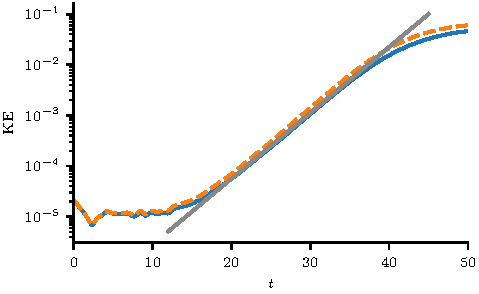
\includegraphics[width=0.5\linewidth]{log_kinetic_energy_over_time.pdf}
  \caption{\textit{Logarithmic plot of the total kinetic
      energy during the linear phase.} Overlaid is a straight
    line corresponding to the linear growth rate $\sigma = 0.13$. The
    isotropic case is represented as a blue, solid line and the
    switching case as an orange, dashed line. Though the kinetic energy is initially slightly greater using the switching model, the growth rate appears unaffected by choice of viscosity model. The duration of the linear phase also appears to be negligibly affected.}%
  \label{fig:log_kinetic_energy_over_time}
\end{figure}

The linear development of the kink instability lasts until $t\approx 35$ as illustrated in   Figure~\ref{fig:log_kinetic_energy_over_time} and has a measured linear growth rate of $\sigma = 0.13$. Since the initial velocity perturbation is calculated from an ideal and inviscid MHD model with a piecewise constant $\alpha(r)$ in the equilibrium configuration, the perturbation does not necessarily represent the most unstable mode for the setup of the simulation. For this reason there is a brief transient period before the exponential rise of the instability at $t\approx10$, as shown in Figure~\ref{fig:log_kinetic_energy_over_time}. The isotropic model damps this initial velocity perturbation more than the switching model, leading to a small difference in kinetic energy during the growth of the linear instability, although the growth rate appears to be identical across the two models. The duration of the linear phase is also unaffected by the choice of viscosity model.

\begin{figure}[t]
  \centering
    \begin{subfigure}{0.49\textwidth}
      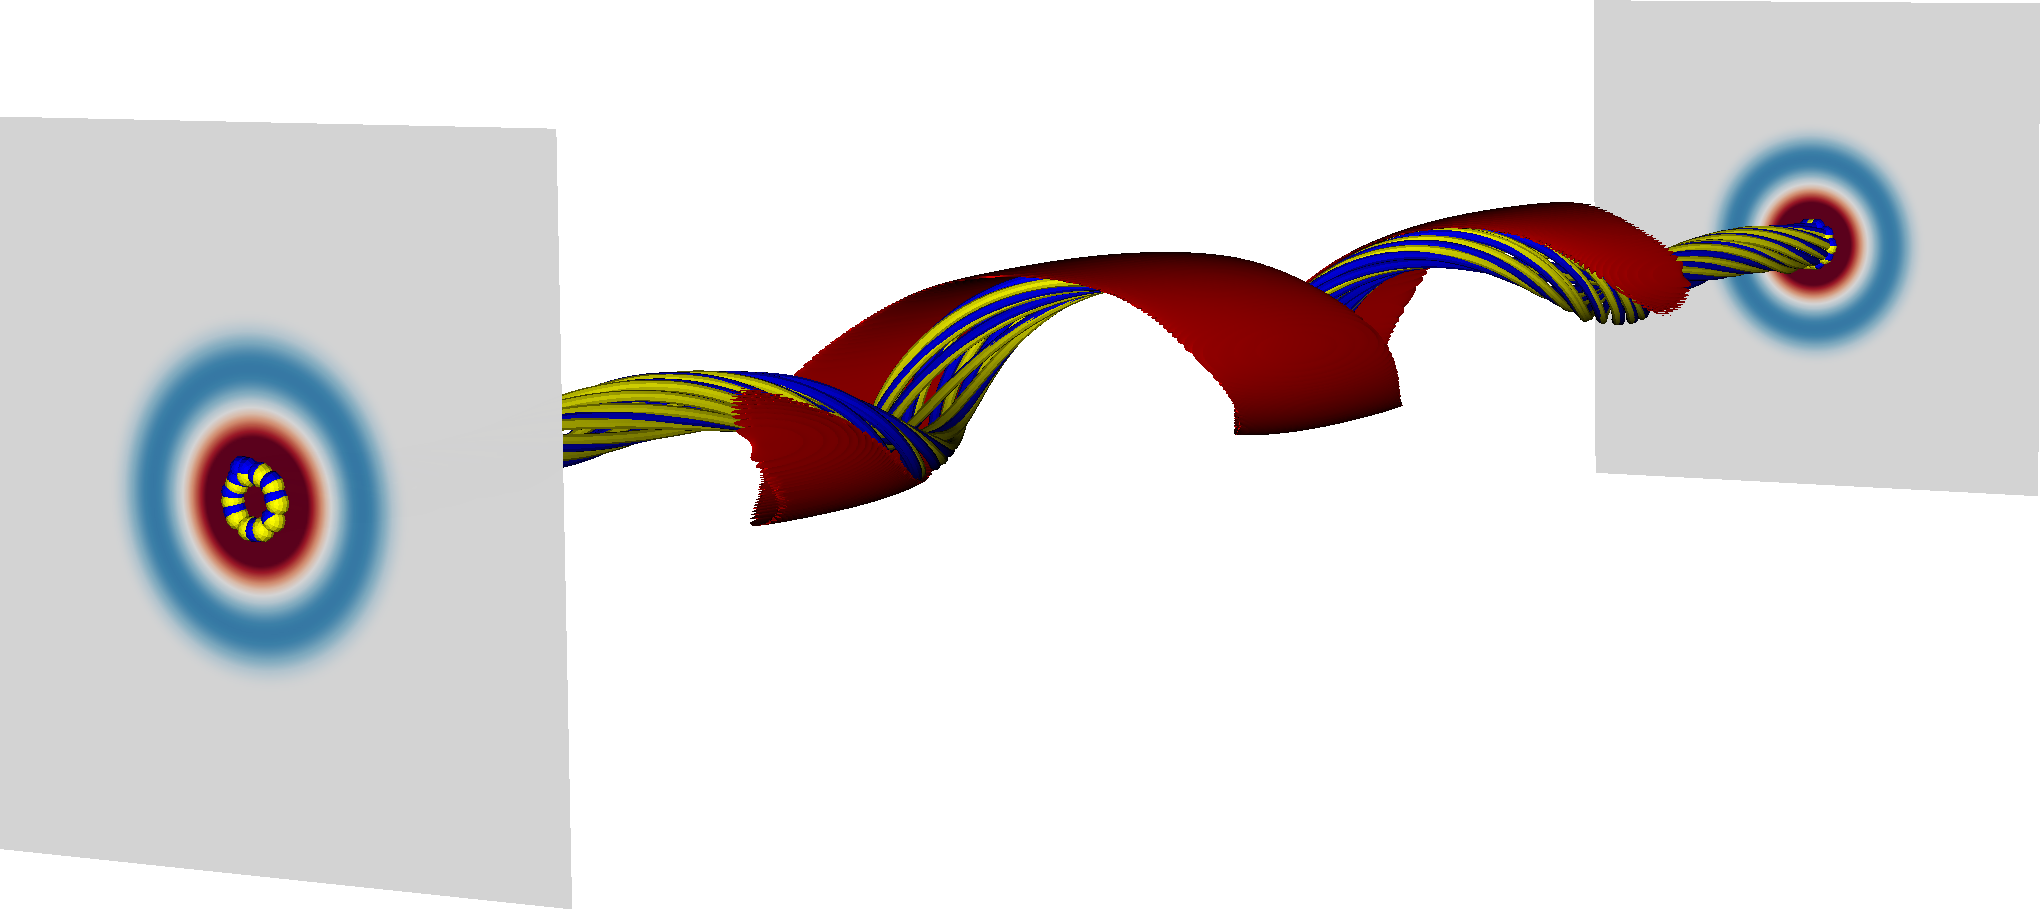
\includegraphics[width=\linewidth]{field_line_plots/cropped/v1e-4r5e-4.5-isotropic_0009_cropped.png}
      \caption{$t=45$}
      \label{fig:field_lines_0009}
    \end{subfigure}
    \begin{subfigure}{0.49\textwidth}
      \includegraphics[width=\linewidth]{field_line_plots/cropped/v1e-4r5e-4.5-isotropic_0010_cropped.png}
      \caption{$t=50$}
      \label{fig:field_lines_0010}
    \end{subfigure}
\caption{\textit{The transition from linear to nonlinear instability in the isotropic case.} The yellow field lines start at $z=10$ and the blue field lines at $z=-10$. The isosurfaces are at $|\vec{\jmath}| = 4$. The slices are plots of $\alpha(r)$. The linear growth of the instability ends around $t=35$ and the inner field compresses into the outer field, creating a current sheet. Between $t=45$ and $50$ this current sheet enables reconnection between the two regions. The transition for the switching case is qualitatively similar. In all three plots, $\nu = 10^{-4}$ and $\eta = 5\times 10^{-4.5}$, respectively.}
\label{fig:reconnecting_field_lines}%
\end{figure}

Initially, the instability occurs in the inner region of twist, $r<0.5$, where the magnetic field kinks helically. This section of the magnetic field compresses into the outer region, creating a current sheet along the length of the tube as shown in Figure~\ref{fig:field_lines_0009}. As the field continues to be compressed, it provides a magnetic pressure force that stalls the linear growth. The greater kinetic energy in the switching case leads to greater compression and thus a larger (though not notably stronger) current sheet. After this point, the growth of the kink instability is no longer in the linear phase.

During the transition from the linear to the nonlinear phase, field lines in the current sheet between the regions of inner and outer twist start to reconnect (Figures~\ref{fig:reconnection-field-lines}). This happens sooner in the switching case, due to the larger compression.

\subsection{Nonlinear phase}

\begin{figure}[t]
    \centering
    \begin{subfigure}[t]{0.49\textwidth}
      \centering
      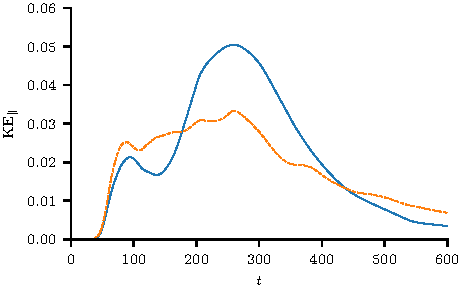
\includegraphics[width=\linewidth]{parallel_kinetic_energy_over_time.pdf}
      \caption{Parallel kinetic energy}
      \label{fig:parallel_kinetic_energy_over_time}
    \end{subfigure}%
    \begin{subfigure}[t]{0.49\textwidth}
      \centering
      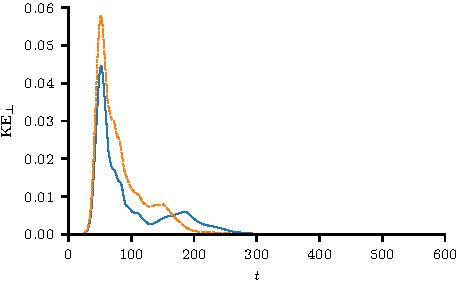
\includegraphics[width=\linewidth]{perp_kinetic_energy_over_time.pdf}
      \caption{Perpendicular kinetic energy}
      \label{fig:perp_kinetic_energy_over_time}
    \end{subfigure}
    \begin{subfigure}[t]{0.49\textwidth}
      \centering
      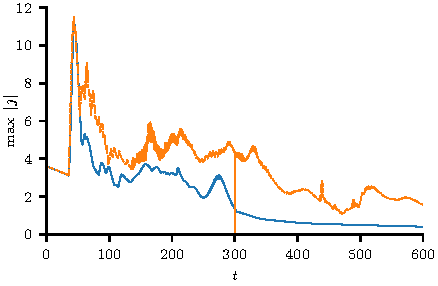
\includegraphics[width=\linewidth]{current_density_over_time.pdf}
      \caption{Maximum current density}
      \label{fig:current_density_over_time}
    \end{subfigure}
    \begin{subfigure}[t]{0.49\textwidth}
      \centering
      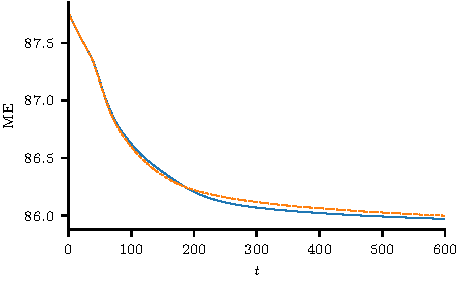
\includegraphics[width=\linewidth]{magnetic_energy_density_over_time.pdf}
      \caption{Magnetic energy}
      \label{fig:magnetic_energy_density_over_time}
    \end{subfigure}
    \caption{\textit{Energy components and current as functions of time.} Both isotropic (blue, solid) and switching (orange, dashed) viscosity models are shown, with diffusion parameters $\nu = 10^{-4}$ and $\eta = 5\times 10^{-4.5}$.}
    \label{fig:energies}
\end{figure}

Although the choice of viscosity model has a small effect on the
linear phase of the kink instability, it does play an important role
in the development of the nonlinear phase. By examining the kinetic
energies (KEs) in Figures~\ref{fig:energies}(a) and (b), a pattern
emerges in both cases that has similarities with the nonlinear
  behaviour of kink instabilities described in Hood et
al.~\cite{hoodCoronalHeatingMagnetic2009}. Shortly after the linear
phase, at $t\approx50$, the KEs for both viscosity models
exhibits a sharp rise, with the KEs associated with the switching
model attaining higher amplitudes. At the same time, a sharp rise is
also found in the maximum current as seen in
Figure~\ref{fig:energies}(c) and, leading on from this spike, the
current magnitudes associated with the switching model are larger than
those associated with the isotropic model. Returning to the KEs, the
energies associated with the switching model are greater until
$t\approx175$, after which, in \emph{only} the isotropic case, 
a clear secondary spike in perpendicular kinetic energy is found, along with a large
increase in parallel kinetic energy, much greater than the corresponding energy
found in the switching case. It is difficult to detect this new phase
in the maximum current (Figure~\ref{fig:energies}(c)), but it is found
in other quantities related to magnetic reconnection. 

\begin{figure}[t]
    \centering
    \begin{subfigure}[t]{0.5\textwidth}
      \centering
      \includegraphics[width=\linewidth]{max_parallel_electric_field.pdf}
      \caption{Parallel electric field}
      \label{fig:max_parallel_electric_field}
    \end{subfigure}%
    ~
    \begin{subfigure}[t]{0.5\textwidth}
      \centering
      \includegraphics[width=\linewidth]{mean_difference_in_connectivity.pdf}
      \caption{Difference in connectivity}
      \label{fig:mean_difference_in_connectivity}
    \end{subfigure}
    \caption{\textit{Reconnection rates.} The maximum integrated parallel electric field and mean difference in connectivity are plotting for the isotropic (blue dot \& solid line) and switching (orange cross \& dashed line) cases with $\nu = 10^{-4}$ and $\eta = 5\times 10^{-4.5}$. The difference in time between each data point is $5$ Alfv\'en times.}
    \label{fig:reconnection-rates}
\end{figure}

Figure~\ref{fig:reconnection-rates} displays the time series of the maximum integrated parallel electric field and the mean difference in connectivity, for both viscosity models. Both of the time series in Figure~\ref{fig:reconnection-rates} display similar trends to those found in the perpendicular kinetic energy plot, Figure~\ref{fig:energies}(a). For both isotropic and anisotropic viscosity there appears to be two major peaks in the reconnection measures that align with peaks in the perpendicular kinetic energy. This is much more obvious in the isotropic case. Both viscosity models allow for two phases of reconnection but the time at which they occur is significantly modified by the form of viscosity chosen. It is, therefore, clear that the form of viscosity is having a significant effect on the nonlinear evolution of the kink instability, both on the flow dynamics and the reconnection of the magnetic field. The following section presents, in more detail, the two important phases indicated by the isotropic time series, and how the results differ in the switching case.

\subsection{First phase: $t\approx65$--$100$}

\begin{figure}[t]
  \centering
  \begin{subfigure}[t]{0.32\textwidth}
    \centering
    \includegraphics[width=\linewidth]{slices/final_isotropic_current_density_0013.pdf}
    \caption{iso; $t=65$}
    \label{fig:final_isotropic_current_density_0013}
  \end{subfigure}
  \hfill
  \begin{subfigure}[t]{0.32\textwidth}
    \centering
    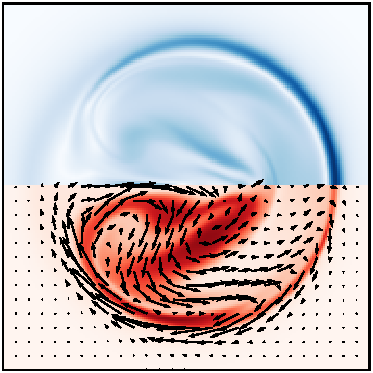
\includegraphics[width=\linewidth]{slices/final_isotropic_current_density_0015.pdf}
    \caption{iso; $t=75$}
    \label{fig:final_isotropic_current_density_0015}
  \end{subfigure}
  \hfill
  \begin{subfigure}[t]{0.32\textwidth}
    \centering
    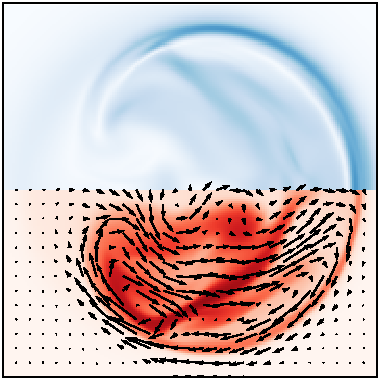
\includegraphics[width=\linewidth]{slices/final_isotropic_current_density_0020.pdf}
    \caption{iso; $t=100$}
    \label{fig:final_isotropic_current_density_0020}
  \end{subfigure}
  \hfill
  \begin{subfigure}[t]{0.32\textwidth}
    \centering
    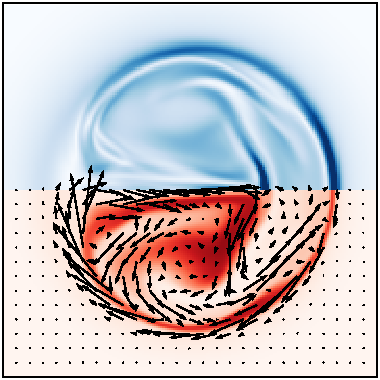
\includegraphics[width=\linewidth]{slices/final_switching_current_density_0013.pdf}
    \caption{swi; $t=65$}
    \label{fig:final_switching_current_density_0013}
  \end{subfigure}
  \hfill
  \begin{subfigure}[t]{0.32\textwidth}
    \centering
    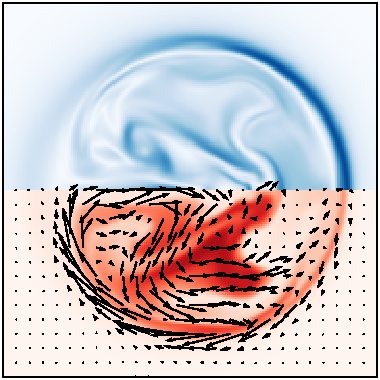
\includegraphics[width=\linewidth]{slices/final_switching_current_density_0015.pdf}
    \caption{swi; $t=75$}
    \label{fig:final_switching_current_density_0015}
  \end{subfigure}
  \hfill
  \begin{subfigure}[t]{0.32\textwidth}
    \centering
    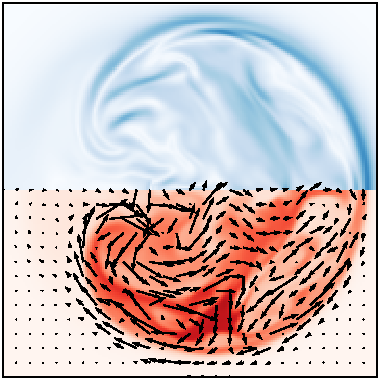
\includegraphics[width=\linewidth]{slices/final_switching_current_density_0020.pdf}
    \caption{swi; $t=100$}
    \label{fig:final_switching_current_density_0020}
  \end{subfigure}
  \caption{\textit{The difference in the evolution of current density,
      temperature and velocity structures between the isotropic
        and the switching viscosity cases}. Slices at $z=0$ of
    current density (top of each figure; blue is $|\vec{\jmath}| =
    3.5$, white is $|\vec{\jmath}| = 0$) and temperature (bottom of
    each figure; red is $T = 5\times10^{-2}$, white is
    $T=1.15\times10^{-5}$), overlaid with fluid flow. The halves shown are identical to their unseen counterparts, for both temperature and current density. That is, the simulation is vertically symmetrical at these times. The profile is cropped to
    $x=\pm1,\ y=\pm1$. The top three panels show the
    isotropic case and the bottom three panels show the switching case.}
  \label{fig:turning-point}
\end{figure}

At $t=65$, an intense current structure appears near the centre of the
tube for both viscosity models, although it is much stronger in the
switching case as illustrated in Figure~\ref{fig:turning-point}. Since the viscous damping associated with parallel viscosity is much less than that of isotropic viscosity, the flows in the switching case are stronger than those in the isotropic case (Figures~\ref{fig:energies}(a) and (b)). The faster flows drive stronger reconnection in the central current structure (see Figure~\ref{fig:reconnection-rates}) and the interaction of these processes leads to stronger outflows and finer-scale structures in the switching model case compared with the isotropic model case. Evidence of this behaviour can be seen by comparing the current and flow structures in Figure~\ref{fig:turning-point}. The effects of this phase can also be seen in the magnetic energy evolution, shown in Figure~\ref{fig:energies}(d). Between times $t=100$ and $125$, due to stronger reconnection in the switching case, the magnetic field relaxes marginally faster than that of the isotropic case, before the secondary instability begins in the isotropic case around $t=125$.

\begin{figure}[t]
  \centering
  \begin{subfigure}[t]{0.32\textwidth}
    \centering
    \includegraphics[width=\linewidth]{slices/final_isotropic_current_density_0025.pdf}
    \caption{iso; $t=125$}
    \label{fig:final_isotropic_current_density_0025}
  \end{subfigure}
  \hfill
  \begin{subfigure}[t]{0.32\textwidth}
    \centering
    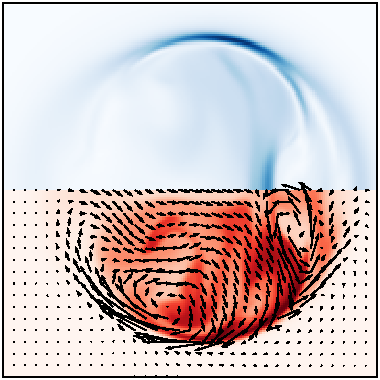
\includegraphics[width=\linewidth]{slices/final_isotropic_current_density_0030.pdf}
    \caption{iso; $t=150$}
    \label{fig:final_isotropic_current_density_0030}
  \end{subfigure}
  \hfill
  \begin{subfigure}[t]{0.32\textwidth}
    \centering
    \includegraphics[width=\linewidth]{slices/final_isotropic_current_density_0035.pdf}
    \caption{iso; $t=175$}
    \label{fig:final_isotropic_current_density_0035}
  \end{subfigure}
  \hfill
  \begin{subfigure}[t]{0.32\textwidth}
    \centering
    \includegraphics[width=\linewidth]{slices/final_switching_current_density_0025.pdf}
    \caption{swi; $t=125$}
    \label{fig:final_switching_current_density_0025}
  \end{subfigure}
  \hfill
  \begin{subfigure}[t]{0.32\textwidth}
    \centering
    \includegraphics[width=\linewidth]{slices/final_switching_current_density_0030.pdf}
    \caption{swi; $t=150$}
    \label{fig:final_switching_current_density_0030}
  \end{subfigure}
  \hfill
  \begin{subfigure}[t]{0.32\textwidth}
    \centering
    \includegraphics[width=\linewidth]{slices/final_switching_current_density_0035.pdf}
    \caption{swi; $t=175$}
    \label{fig:final_switching_current_density_0035}
  \end{subfigure}
  \caption{\textit{The formation of a reconnection feedback loop in the isotropic and the switching viscosity cases.} Plotting parameters are identical to those of Figure~\ref{fig:turning-point}. The isotropic case shows two current sheets causing reconnection at the top and bottom of the tube, producing flows that sustains another central current sheet, which feeds back into the top and bottom sheets. The switching case instead shows one single main current sheet at the right hand side, along with numerous smaller current structures throughout the domain.}
  \label{fig:feedback-reconnection}
\end{figure}

\subsection{Second phase: $t\approx125$--$175$}
The contrast between fine-scale current and flow structures for the switching model, and the smoother, larger-scale structures of the isotropic model continues to be present at later times. Figure~\ref{fig:feedback-reconnection} shows the same data as Figure~\ref{fig:turning-point} but for the times $t=125$, $150$ and $175$. Looking at the slices for $t=125$, there is more fine-scale structure generated in the switching case compared to the isotropic case, as in the first phase described above. This second phase, however, marks the beginning of a significant change in behaviour in the isotropic model case. From Figure~\ref{fig:energies}, the parallel KE for the isotropic model exhibits a rapid and large increase in kinetic energy, characteristic of a secondary instability. To a lesser extent, there is also growth in the perpendicular KE, and the two reconnection measures for the isotropic model. In the second phase, these three measures increase to eventually become greater than their corresponding values for the switching model, around $t=175$. The significant difference in the behaviour between the two models are explored by first considering the slices in Figure~\ref{fig:feedback-reconnection}.

\begin{figure}[t]
  \centering
  \begin{subfigure}[b]{0.48\textwidth}
    \includegraphics[width=\linewidth]{field_line_plots/cropped/v1e-4r5e-4.5-isotropic_0035_cropped.png}
    \caption{Isotropic}
    \label{fig:reconnection-field-lines-iso}
  \end{subfigure}
  \begin{subfigure}[b]{0.48\textwidth}
    \includegraphics[width=\linewidth]{field_line_plots/cropped/v1e-4r5e-4.5-switching_0035_cropped.png}
    \caption{Switching}
    \label{fig:reconnection-field-lines-swi}
  \end{subfigure}
  \caption{\textit{The difference in 3D current structures at $t=175$.} Isosurfaces are at $|\vec{\jmath}| = 1.5$.}
\label{fig:reconnection-field-lines}
\end{figure}

At $t=125$ (panels (a) and (d) of Figure~\ref{fig:feedback-reconnection}), the difference in behaviour
between the models is similar to the first phase but some new features
appear. The KE in the isotropic model begins to increase and, as
mentioned before, appears to signify a secondary instability. In
Figure~\ref{fig:feedback-reconnection}(a), two new current sheets have
formed at the top and bottom of the tube. A three-dimensional (3D)
visualisation of these current sheets is shown in
Figure~\ref{fig:reconnection-field-lines-iso}. The outflow from the
reconnection occurring within these current sheets then creates two
new symmetric vortices on the right hand side of the tube, advecting
the field into the centre of the tube. This behaviour can be seen
clearly in Figure~\ref{fig:feedback-reconnection}(b) where vortex
motion compresses the magnetic field and forms a central region of
enhanced current density. Later, as seen at $t=175$ in Figure~\ref{fig:feedback-reconnection}(c), the central current region becomes stronger due to continued compression and reconnection ensues, becoming stronger than the switching model case (see Figure~\ref{fig:reconnection-rates}). The outflows from this current region then feed into the vortical motions that drive the compression. In this way, a feedback loop is set up, and the reconnection within the current structure continuously drives the flow, resulting in an instability. This kind of interaction between multiple current sheets is also seen in~\cite{hoodCoronalHeatingMagnetic2009}. Due to this secondary instability, magnetic relaxation now becomes faster for the isotropic case. The magnetic energy for this case now dips below that of the switching case, as shown in Figure~\ref{fig:energies}(d).

During this phase, the kinetic energy in the switching model case also increases but to a much smaller extent compared to the isotropic model case. Although the current densities in Figures~\ref{fig:feedback-reconnection}(d) to (f) again exhibit finer-scale structure compared to the isotropic case, the magnitude of the current density within the tube becomes weaker with a more uniform profile developing in time. The dominating current sheets are on the edge of the tube, as also indicated in Figure~\ref{fig:reconnection-field-lines-swi}.

\subsection{Late-time states}

\begin{figure}[t]
  \centering
  \begin{subfigure}[b]{0.48\textwidth}
    \includegraphics[width=\linewidth]{field_line_plots/cropped/v1e-4r5e-4.5-isotropic_0062_cropped.png}
    \caption{Isotropic}
  \end{subfigure}
  \begin{subfigure}[b]{0.48\textwidth}
    \includegraphics[width=\linewidth]{field_line_plots/cropped/v1e-4r5e-4.5-switching_0059_cropped.png}
    \caption{Switching}
  \end{subfigure}
  \caption{\textit{Late-time magnetic field structures at $t=600$.}}
\label{fig:finale-field-lines}
\end{figure}

For both cases, the asymptotic relaxed magnetic field is a linear force-free field. The route to this asymptotic state, however, depends on the viscosity model used. At the late time of $t=600$, there remain clear differences in the field structure between the two models resulting from the different nonlinear evolutions, as can be seen in Figure~\ref{fig:finale-field-lines}. At $t=600$, the magnetic field in the isotropic case (Figure~\ref{fig:finale-field-lines}(a)) appears straighter, indicative of more efficient magnetic relaxation. Indeed, Figure~\ref{fig:energies}(d) shows that more energy has been extracted from the field in the isotropic case. At $t=600$, the current density and energies (see Figure~\ref{fig:energies}) are still non-zero, so further relaxation is expected. For coronal applications, however, these late times are not as important as the early phases, described above, when the initial and secondary instabilities develop.

\subsection{Viscous and Ohmic heating}

\begin{figure}[t]
    \centering
    \begin{subfigure}[t]{0.32\textwidth}
      \includegraphics[width=\textwidth]{ohmic_heating_over_time.pdf}
      \caption{Ohmic heating}
    \end{subfigure}
    \begin{subfigure}[t]{0.32\textwidth}
      \includegraphics[width=\textwidth]{viscous_heating_over_time.pdf}
      \caption{Viscous heating}
    \end{subfigure}
    \begin{subfigure}[t]{0.32\textwidth}
      \includegraphics[width=\textwidth]{total_heating_over_time.pdf}
      \caption{Total heating}
    \end{subfigure}
    \caption{\textit{Heating rates as functions of time.} Plots are shown for isotropic (blue, solid) and switching (orange, dashed) viscosity, with diffusion parameters $\nu = 10^{-4}$ and $\eta = 5\times 10^{-4.5}$. Ohmic heating dominates isotropic viscous heating by an order of magnitude, and switching viscosity by four orders. Isotropic viscosity generates a factor of around $10^{3}$ more heat that switching viscosity. Even though more Ohmic heat is generated in the switching case, it does not compensate for the much weaker viscous heating.}
    \label{fig:heating}
\end{figure}

Over the lifetime of the entire instability the switching model allows for the generation of more Ohmic heating (Figure~\ref{fig:heating}(a)). This is despite the long, secondary phase of reconnection produced in the isotropic case. The greater heating in the switching case is due to two factors: the greater compression created by faster flows, creating stronger or larger current sheets and the more numerous current sheets created by more complex flows. However, isotropic viscous heating dominates that of the switching model by two orders of magnitude (Figure~\ref{fig:heating}(b)) ultimately leading to greater overall heating in the isotropic case (Figure~\ref{fig:heating}(c)). Physically, this is due to anisotropic viscosity only performing significant damping when velocity gradients align appropriately with the magnetic field (that is, when $(\ten{W} \vec{b}) \cdot \vec{b}$ is non-zero). 

Comparing Ohmic and viscous heating (Figures~\ref{fig:heating}(a) and (b)), Ohmic heating outperforms viscous heating in both cases, by an order of magnitude in the isotropic case and by three orders in the switching case. Even though similar values for the diffusion of the magnetic field $\eta$ and the velocity $\nu$ are used, during the kink instability the current sheets produced are much stronger than the gradients in velocity, hence the Ohmic heating dissipates more energy than the viscous heating.

Due to the relationship between $(\ten{W} \vec{b}) \cdot \vec{b}$ and $Q_{\nu}$ (equation~\eqref{eq:aniso_viscous_heating} with $s\approx 1$), the small magnitude of $Q_{\nu}$ in Figure~\ref{fig:heating}(b) implies that $(\ten{W} \vec{b}) \cdot \vec{b}$ is small everywhere. With the anisotropic viscous heating being heavily dependent on the magnetic field direction and since $(\ten{W} \vec{b}) \cdot \vec{b}$ is small everywhere in the kink simulation, it follows that the anisotropic viscous heating is always lower in magnitude compared to the isotropic viscous heating, which is not bound by the diection of the magnetic field.

\subsection{The effect of anisotropy on feedback reconnection}

I have described the nonlinear evolution of the kink instability for the cases of only isotropic viscosity and only anisotropic viscosity. When the viscosity is totally isotropic, the secondary instability is found, yet when the viscosity is totally anisotropic, the same instability is disrupted. To determine how anisotropic the viscosity must become before the secondary instability is disrupted, the degree of anisotropy can be fixed by artificially fixing the value of $s$ to some constant, instead of letting $s$ rely on the local field strength $|\vec{B}|$. It should be noted that the simulations in which $s$ is fixed are no longer physically realistic, but the results can be used to estimate the degree of anisotropy required in the viscosity to disrupt the secondary instability. Since the interpolation involves only $s^2$ instead of $s$, in practice the value of $s^2$ is fixed.

\begin{figure}[t]
  \centering
  \includegraphics[width=0.5\linewidth]{kinetic-energy-changing-s.pdf}
  \caption{\textit{Kinetic energy over time, varying the switching
        function $s^2$.} The grey lines are the two regular cases; switching, where $s^2 = 1$ (dashed), and isotropic (solid), where $s^2=0$. The coloured lines represent values of $s^2 = 0.5$ (blue, dotted), and $s^2 = 0.6$ (orange, dash-dotted). There is a clear critical value somewhere between $0.5$ and $0.6$, where the behaviour changes.}
  \label{fig:kinetic-energy-changing-s}
\end{figure}

By letting $s^2$ in equation~\eqref{eq:switching_model} take values between $0$ and $1$, it is found that there is not a smooth transition between the two extremes of behaviour. Instead, there is a critical value of $s^2$, between $0.5$ and $0.6$, below which (closer to isotropic) the resultant flows are simple enough to create and sustain feedback reconnection, and above which (closer to anisotropic) the flows are sufficiently complex to disrupt the secondary instability. This behaviour can be seen in how the kinetic energy time series changes with $s^2$ in Figure~\ref{fig:kinetic-energy-changing-s}.

\section{Parameter study}
\label{sec:results2}

In order to confirm that the results of Section~\ref{sec:results} are typical, and to further understand how they vary, two parameter studies are performed; one varying viscosity, keeping all other parameters constant; and one varying resistivity, again keeping all other parameters constant. 

In the first study the viscosity is varied as $\nu = 5 \times 10^{-n}$, where the index $n$ takes the values $4.75$, $4.5$, $4.25$, $4$ and $3.75$, while keeping resistivity constant at $\eta = 5\times10^{-4.5}$. This range of viscosities represents values that are typically used in simulations, with a lower bound above numerical diffusion and an upper bound below physically unrealistic values for the corona.

In the second study the resistivity is similarly varied as $\eta = 5 \times 10^{-m}$, where the index $m$ takes the values $4.75$, $4.5$, $4.25$, $4$, $3.75$, and $3.5$, while keeping the resistivity constant at $\nu = 5\times 10^{-4.5}$. Similar to the limits on viscosity, any lower resistivities become comparable to numerical diffusion. Higher resistivities diffuse the field so quickly that the instability does not have time to grow.

\subsection{Effect on the secondary instability varying diffusion parameters}
\label{sec:secondary_instability}

\begin{figure}[t]
    \centering
    \begin{subfigure}[t]{0.5\textwidth}
      \includegraphics[width=\textwidth]{max_ke_split_inst_changing_viscosity.pdf}
      \caption{Varying viscosity; $\eta = 5\time 10^{-4.5}$}
    \end{subfigure}%
    ~
    \begin{subfigure}[t]{0.5\textwidth}
      \includegraphics[width=\textwidth]{max_ke_split_inst_changing_resistivity.pdf}
      \caption{Varying resistivity; $\nu = 5\time 10^{-4.5}$}
    \end{subfigure}
    \caption{\textit{Maximum kinetic energy corresponding to initial instability and secondary instability as functions of resistivity $\eta$ and viscosity $\nu$.} In both plots are shown the maximum kinetic energy produced by the initial instability (green, $1$-marker) and the maximum kinetic energy produced by the secondary instability (purple, $2$-marker). Only results using the isotropic viscosity are shown.}
    \label{fig:secondary_instability}
\end{figure}

Figure~\ref{fig:secondary_instability} shows the maximum kinetic energy produced by the two instabilities found in the isotropic case in Section~\ref{sec:results}. The maximum kinetic energy provides a useful measure of the efficacy of an instability, particularly when comparing the relative magnitudes of the initial and secondary instabilities. Since only the isotropic case reveals evidence of the secondary instability, results from the switching case are not shown.

Looking at Figure~\ref{fig:secondary_instability}(a), it is observed that increasing $\nu$ reduces the kinetic energy generated in both instabilities. For small values of $\nu$ the secondary instability causes more energy to be produced than the first, however as $\nu$ increases, this relationship reverses, with the initial instability causing more energy to be produced than the secondary one for large $\nu$. This reversal suggests that the greater kinetic energy produced by the initial instability for low values of $\nu$ is causing a stronger current sheet to form, enhancing reconnection, and producing a stronger secondary instability.

The effect of resistivity $\eta$ on the secondary instability is to suppress it entirely when $\eta$ is large. Since the secondary instability is driven by reconnection outflows, it is not surprising that there are values of $\eta$ for which the reconnection outflows do not feedback to produce the instability.

\subsection{Varying viscosity}

\label{sec:visc_param_study}

\subsubsection{Dependence of heating on viscosity}

\begin{figure}[t]
    \centering
    \begin{subfigure}[t]{0.32\textwidth}
      \includegraphics[width=\textwidth]{visc_heating_varying_viscosity.pdf}
      \caption{Viscous heating}
    \end{subfigure}%
    ~
    \begin{subfigure}[t]{0.32\textwidth}
      \includegraphics[width=\textwidth]{ohmic_heating_varying_viscosity.pdf}
      \caption{Ohmic heating}
    \end{subfigure}
    ~
    \begin{subfigure}[t]{0.32\textwidth}
      \includegraphics[width=\textwidth]{max_kinetic_changing_visc.pdf}
      \caption{Maximum kinetic energy}
    \end{subfigure}
    \caption{\textit{Anisotropic viscous heating, Ohmic heating, and maximum kinetic energy as functions of viscosity $\nu$.} Plots are shown using isotropic viscosity (blue, solid) and switching viscosity (orange, dashed) as functions of viscosity $\nu$ at the final time of $t=400$ for a fixed resistivity $\eta=5\times10^{-4.5}$, The anisotropic viscous heating has been multiplied by a factor of $10$. The maximum kinetic energy is calculated as the maximum value prior to $t=400$.}
    \label{fig:param_study_varying_viscosity}
\end{figure}

Figures~\ref{fig:param_study_varying_viscosity}(a) and~\ref{fig:param_study_varying_viscosity}(b) show the total heat generated by $t=400$ via viscous $Q_{\nu}$ and Ohmic $Q_{\eta}$ dissipation as $\nu$ is varied. It should be noted that, to allow the trend in the anisotropic viscous heating to be seen in the plot, it has been multiplied by a factor of $10$. Before discussing the apparent trends in the heating as $\nu$ is varied, it is useful to note that, just as in the typical case described previously, for the range of $\nu$ shown, isotropic viscous heating remains approximately two orders of magnitude greater than the anisotropic viscous heating, and the Ohmic heating is consistently higher when using anisotropic viscosity than when using isotropic.

Since viscous dissipation (equations~\eqref{eq:iso_viscous_heating} and~\eqref{eq:aniso_viscous_heating}) has a functional dependence on $\nu$ and Ohmic dissipation (equation~\eqref{eq:ohmic_heating}) does not, it could be naively assumed that variation in viscosity should present some trend in the viscous dissipation for both models and no trend in the Ohmic dissipation. The trends that are observed broadly adhere to this but, unexpectedly there appears some trend in the Ohmic heating when using isotropic viscosity.

When employing the switching model, the Ohmic heating appears to be independent of $\nu$, whereas when employing the isotropic model, there appears a small trend of decreased Ohmic heating with increased $\nu$. These trends can be explained by considering the effect of viscosity on compressive flows and current densities. During the kink instability, Ohmic heating, being proportional to the square of the local current density, is increased when an already sheared magnetic field is compressed by flows perpendicular to the field, increasing the local current density. Thus, as the speeds of perpendicular flows increase, so does the Ohmic heating. These perpendicular flows are effectively only damped by isotropic viscosity. Since the maximum kinetic energy (Figure~\ref{fig:param_study_varying_viscosity}(c)) decreases with $\nu$ in \emph{only} the isotropic case, and remains constant in the switching case, it is appropriate that the Ohmic heating decreases with $\nu$ in the isotropic case and is negligibly dependent on $\nu$ in the switching case.

If varying $\nu$ does not change the dynamics in the switching case, the functional dependence of $Q_{\nu}$ on $\nu$ (see equation~\eqref{eq:aniso_viscous_heating}) suggests an increase in anisotropic viscous heating with $\nu$ should be observed. Figure~\ref{fig:param_study_varying_viscosity}(a) reveals precisely this.

The relationship between the isotropic viscous heating at $\nu$ appears non-trivial. Given the decrease in maximum kinetic energy (Figure~\ref{fig:param_study_varying_viscosity}(a)) with $\nu$, it is expected the isotropic viscous heating should also decrease. However, this is not what is observed. Although there appears to be a slight decreasing trend in the isotropic viscous heating when $\nu$ is increased past $10^{-4}$, the left-most point is clearly an outlier. This suggests the secondary instability is having a significant and non-trivial effect on the heating. Indeed this is also suggested by the subtle change of gradient in the maximum kinetic energy on the left-hand side of the Figure~\ref{fig:param_study_varying_viscosity}(c). Due to this particular parameter study producing only five data points, these trends cannot be discussed with much confidence. A more detailed parameter study should be performed, investigating more values of $\nu$ within and beyond the range studied here.

\subsubsection{Dependence of linear growth rate on viscosity}
\label{sec:linear_growth_rate_varying_visc}

\begin{figure}[t]
    \centering
    \begin{subfigure}[t]{0.5\textwidth}
      \includegraphics[width=\textwidth]{growth_rate_varying_viscosity.pdf}
      \caption{Growth rate}
    \end{subfigure}%
    ~
    \begin{subfigure}[t]{0.5\textwidth}
      \includegraphics[width=\textwidth]{max_early_time_kinetic_changing_visc.pdf}
      \caption{Maximum early-time kinetic energy}
    \end{subfigure}
    \caption{\textit{Linear growth rate and maximum (in time) kinetic energy as
        functions of viscosity $\nu$ for a fixed
          resistivity of $\eta=5\times10^{-4.5}$.} Plots are shown using isotropic viscosity (blue, solid) and switching viscosity (orange, dashed) as functions of viscosity $\nu$. The maximum kinetic energies are calculated as the maximum values in time prior to $t=125$. This is to capture the behaviour of only the initial nonlinear evolution of the instability, neglecting any further instabilities like the secondary instability found in Section~\ref{sec:results}. Note, the maxima do not necessarily occur at the same time and this particular parameter study has been performed fixing $\nu$ at a slightly different value to the previous parameter studies.}
    \label{fig:growth_rate_varying_viscosity}
\end{figure}

For each value of $\eta$ the linear growth rate $\sigma$ of the onset of the kink instability is estimated by plotting the logarithm of the kinetic energy against time and measuring the gradient during the period of linear growth (as is done in Figure~\ref{fig:log_kinetic_energy_over_time}). Figure~\ref{fig:growth_rate_varying_viscosity}(a) plots these growth rates against $\eta$, and Figure~\ref{fig:growth_rate_varying_viscosity}(b) shows the maximum kinetic energy calculated as the maximum prior to $t=125$. For every $\eta$, this time is between the peaks of the kinetic energy corresponding to the first and secondary instabilities. Taking the maximum before this time allows us to capture only the behaviour of the initial instability, since this is the instability of interest in this section.

It can be seen from the relationship between the growth rate and $\nu$ for both viscosity models that isotropic viscosity appears to begin to suppress the kink instability, for larger $\nu$, while the switching viscosity does not (Figure~\ref{fig:growth_rate_varying_viscosity}(a)). This is also apparent from the relationship between the maximum kinetic energy and $\nu$ for both models (Figure~\ref{fig:growth_rate_varying_viscosity}(b)). This difference between the viscosity models results from the anisotropic viscosity being so weak that the dynamics of the initial onset of the kink instability are not significantly affected by a significant increase in $\nu$.

\subsection{Varying resistivity}

\subsubsection{Dependence of heating on resistivity}

\begin{figure}[t]
    \centering
    \begin{subfigure}[t]{0.5\textwidth}
      \includegraphics[width=\textwidth]{visc_heating_varying_resistivity.pdf}
      \caption{Viscous heating}
    \end{subfigure}%
    ~
    \begin{subfigure}[t]{0.5\textwidth}
      \includegraphics[width=\textwidth]{ohmic_heating_varying_resistivity.pdf}
      \caption{Ohmic heating}
    \end{subfigure}
    \caption{\textit{Anisotropic viscous, and Ohmic heating as functions of resistivity $\eta$ for a fixed value of viscosity $\nu=5\times10^{-4.5}$.} Plots are shown using isotropic viscosity (blue, solid) and switching viscosity (orange, dashed) as functions of resistivity $\eta$ at the final time of $t=400$. The anisotropic viscous heating has been multiplied by a factor of $10$. Overlaid on Figure (b) is the scaling $\log_{10}(\eta^{1/2})$.}
    \label{fig:param_study_varying_resistivity}
\end{figure}

Figure~\ref{fig:param_study_varying_resistivity}(a) and~\ref{fig:param_study_varying_resistivity}(b) show the total heating generated by $t=400$ via viscous $Q_{\nu}$ and Ohmic $Q_{\eta}$ dissipation as the strength of resistivity $\eta$ is varied. Just as in Section~\ref{sec:visc_param_study}, the anisotropic viscous heating is multiplied by $10$. Again, it is useful to note that, across the entire range of $\eta$ studied here, the isotropic viscous heating remains approximately two orders of magnitude greater than the anisotropic viscous heating and the Ohmic heating produced when using switching viscosity is consistently higher than that produced when using isotropic viscosity. This aligns with the results when varying viscosity, as discussed above.

As in the parameter study varying $\nu$, a non-trivial relationship appears between the viscous heating for both models and $\eta$ (Figure~\ref{fig:param_study_varying_resistivity}(a)). The isotropic viscous heating reveals an decreasing trend over all values of $\eta$ studies here, however there is a clear jump in heating between approximately $10^{-3.9}$ and $10^{-3.7}$. Given that these are the values of $\eta$ where there is strong influence of the secondary instability on the kinetic energy output (see Section~\ref{sec:secondary_instability}), these results suggest it is the kinetic energy produced by the secondary instability that is being damped at low values of $\eta$.

Just as in the parameter study varying $\nu$, the anisotropic viscosity shows very little variability with $\eta$ (Figure~\ref{fig:param_study_varying_resistivity}(a)), even with the heating multiplied by a factor of $10$ for plotting. Despite the dynamics significantly changing with $\eta$, the effect of the anisotropic viscosity is so small that very little change in the heating is observed.

Ohmic heating is observed to increase with increasing $\eta$ (Figure~\ref{fig:param_study_varying_resistivity}(b)). This is to be expected given the functional dependence of $Q_{\eta}$ on $\eta$, however the actual scaling is not linear in $\eta$, as might be predicted from equation~\eqref{eq:ohmic_heating}. Rather, $Q_{\nu}$ varies linearly with $\log_{10}(\eta^{1/2})$ for the range of $\eta$ studied here. Without a more comprehensive parameter study covering more values of $\eta$, it is difficult to reason why the scaling takes this form. However, what is certain is that the use of anisotropic viscosity is consistently enhancing Ohmic heating across the range of $\eta$ studied here. This is due to the kink instability producing more kinetic energy in the switching case, which better compresses the magnetic field, creating stronger current sheets and thus enhancing Ohmic heating.

\subsubsection{Dependence of linear growth rate on resistivity}

\begin{figure}[t]
    \centering
    \begin{subfigure}[t]{0.5\textwidth}
      \includegraphics[width=\textwidth]{growth_rate_varying_resistivity.pdf}
      \caption{Growth rate}
    \end{subfigure}%
    ~
    \begin{subfigure}[t]{0.5\textwidth}
      \includegraphics[width=\textwidth]{max_kinetic_changing_resist.pdf}
      \caption{Maximum early-time kinetic energy}
    \end{subfigure}
    \caption{\textit{Linear growth rate and maximum (in time) kinetic energy as
        functions of resistivity $\eta$ for a fixed
          viscosity of $\nu=10^{-4}$.} \textbf{(a)} Growth rate and \textbf{(b)} maximum kinetic energy, generated by isotropic viscosity (blue, solid) and switching viscosity (orange, dashed) as functions of resistivity $\eta$. The maximum kinetic energies are calculated as the maximum values in time prior to $t=125$. This is to capture the behaviour of only the initial nonlinear evolution of the instability, neglecting any further instabilities like the secondary instability found in Section~\ref{sec:results}. Note, the maxima do not necessarily occur at the same time and this particular parameter study has been performed fixing $\nu$ at a slightly different value to the previous parameter studies.}
    \label{fig:growth_rate_varying_resistivity}
\end{figure}

As is done in Section~\ref{sec:linear_growth_rate_varying_visc}, the linear growth rates are measured for each value of $\eta$. These and the maximum early time ($t<125$) kinetic energy are shown in Figure~\ref{fig:growth_rate_varying_resistivity}. The plots show that the use of the switching model seems to consistently amplify the growth of the kink instability, shown both in the growth rate and in the kinetic energy. Beyond this, the two models of viscosity show similar trends with $\eta$.

Both plots in Figure \ref{fig:growth_rate_varying_resistivity} show that the kink instability is strongly inhibited for values of $\eta$ greater than approximately $10^{-2.5}$. This can be explained by the initial diffusion of the magnetic field being so fast-acting for large values of $\eta$ that the instability is totally suppressed. The increased suppression of the instability with strength of Ohmic diffusion can be seen in both plots as $\eta$ increases past $10^{-3}$.

\section{Discussion}

\todo{split text from summary into discussion and conclusion}

\section{Conclusion}

\section{Summary and discussion}
\label{sec:conclusions}

This chapter details the linear and nonlinear development of the MHD kink
instability with two different viscosity models. The first is
isotropic (Newtonian) viscosity, which is the most commonly used
viscosity model in coronal loop studies. The second is anisotropic viscosity, representing the strong-field limit of Bragkinskii viscosity with a preferred direction parallel to the magnetic field. The implementation of anisotropic viscosity is via the switching model~\cite{mactaggartBraginskiiMagnetohydrodynamicsArbitrary2017} which is suitable for coronal applications.

By considering particular (low) values of the viscosity and resistivity, it is found that the effect of the different viscosity models on the linear onset of the kink instability is marginal. The significant differences appear in the nonlinear phase. Two main phases of evolution can be identified which highlight the differences between the effects of the two viscosity models. The anisotropic (switching) case produces more kinetic energy at the onset of the nonlinear phase of the instability---the first phase. It also produces flows and current sheets with smaller length scales compared to the isotropic case and this allows the magnetic field to relax faster due to more efficient reconnection. 

In the second phase, the isotropic case exhibits a secondary instability, which is not found in the anisotropic case. This new instability leads to enhanced reconnection and faster magnetic relaxation, compared to the anisotropic case.  The simulations are run for $600$ Alfv\'en times (a long time period for coronal applications) and the behaviour of the second phase continues for all of this time.

A series of parameter studies was also run, where the strengths of viscosity and resistivity were varied. The qualitative results of the two phases of the detailed investigation hold true over a range of viscosities and resistivities, including the existence of the secondary instability. Notably, over all parameters studied, viscous heating is consistently overestimated by the isotropic model, and Ohmic heating is consistently enhanced by use of the switching model.

Although there can be much variability in the nonlinear behaviour of the kink instability, these results reveal an important general finding. At the beginning of the nonlinear phase, anisotropic (parallel) viscosity allows for the development of smaller length scales (both flows and current sheets), compared to isotropic viscosity, leading to more efficient reconnection and faster magnetic relaxation, at least initially. As has been described in detail, isotropic viscosity can produce other effects later. However, for coronal applications, it is the initial nonlinear phase of the instability that is likely to be of most interest since, in reality, a coronal loop will interact with others on a longer time scale, thus affecting the nonlinear evolution. Since anisotropic viscosity is a more realistic model for viscosity in the corona, these results will be useful in the interpretation of observations of coronal loops that are kink unstable.

\chapter{Application to a dynamically twisted flux tube}

\label{chp:kink_instability_straight}

\graphicspath{{images/kink_instability_straight/}}

\section{Introduction}

In chapter~\ref{chp:kink_instability} the dynamics in a magnetic flux rope which is already linearly unstable to the helical kink instability were investigated. An alternative way to excite the kink instability is to start with an initially straight field and apply twisting motions at the boundaries to create a twisted flux rope which eventually becomes unstable to the kink instability. In addition, a fluting instability is found to be excited prior to the development of the kink instability. To our knowledge, this is the first time a fluting instability in coronal conditions has been studied through 3D numerical simulations. 

The fluting instability arises in magnetised plasmas where the plasma pressure gradient is directed in the same direction as the field line curvature, that is the pressure and magnetic tension forces compete. This is similar to the competition between pressure and gravitational forces which gives rise to the Rayleigh-Taylor instability (RTI). In a twisted flux tube like a coronal loop, the tube may be unstable to fluting when the pressure decreases outwards from the core. The ideal fluting instability is simply an ideal interchange instability in a cylindrical flux tube. \todo{ref to later plot of field lines + pressure contours}

In the study of coronal loops, the main focus has been the ideal kink instability (see chapter~\ref{chp:kink_instability}). We do not know of any coronal studies of the fluting instability specifically in coronal loops. In other solar contexts, we find interchange instabilities in the form of ballooning modes in arcades~\cite{hoodBallooningInstabilitiesSolar1986}, as the instability which forms tubes of specific size in the photosphere~\cite{bunteInterchangeInstabilitySolar1993} and in the buoyancy of flux tubes~\cite{schuesslerInterchangeInstabilitySmall1984}. The instability is more commonly studied in fusion contexts.

While the stability of the ideal fluting instability has been studied extensively in fusion research~\cite{mikhailovskiiInstabilitiesConfinedPlasma1998,zhengAdvancedTokamakStability2015,wessonHydromagneticStabilityTokamaks1978}, the focus is generally on understanding how a particular plasma device may be stabilised to the instability in particular geometries such as that of the mirror machine~\cite{jungwirthTheoryFluteInstability1965} or in toroidal geometries such as the tokomak~\cite{shafranovFluteInstabilityCurrentcarrying1968}. The resistive interchange instability (the resistive form of the fluting instability) can be excited even when the ideal fluting instability is stabilised. As a result, this has been given significantly more attention~\cite{johnsonResistiveInterchangesNegativeV1967,correa-restrepoResistiveBallooningModes1983}.

\subsection{Introduction to fluting stability}

In general, the stability of a cylindrical twisted magnetic flux tube is analysed using perturbations of the form
\begin{equation}
  \label{eq:kink_perturbation}
\xi(r, \theta, z) = \xi(r) e^{i(m\theta + kz)},
\end{equation}
where $m$ and $k$ are the wavenumbers in the $\theta$ and $k$ directions, respectively. The helical kink instability occurs for perturbations where $m=1, k\ne0$ and is the only instability of this form which is a body instability, that is it moves the entire body of the flux tube. Perturbations where $m>1$ are fluting or interchange instabilities.

When the magnetic field is sheared, as in a twisted magnetic flux tube, an interchange instability (such as the fluting instability) is confined to a surface where the peaks and troughs follow the shear of the field. That is, a surface where the perturbation wavevector $(0, m/r, k)$ is perpendicular to the direction of the field. In an axisymmetric, twisted flux tube the resonant surface is located at a radius $r$ given by
\begin{equation}
  \label{eq:resonant_surface}
\frac{m}{r} B_{\theta}(r) + kB_z(r) \approx 0.
\end{equation}
In contrast to kink instabilities, fluting instabilities are surface instabilities.

The stability of a cylindrical flux tube to perturbations of the form~\ref{eq:kink_perturbation} is given by the classical Suydam's criterion
\begin{equation}
  \label{eq:suydams_criterion}
\frac{B_z^2 S^2}{4} + 2 r p' > 0,
\end{equation}
where $S = r q'/q$ is a measure of the shear, $q = 2\pi r B_z / L B_{\theta}$ is the safety factor for a flux tube of length $L$~\cite{mikhailovskiiInstabilitiesConfinedPlasma1998} and a dash denotes differentiation with respect to $r$. Where~\ref{eq:suydams_criterion} is unsatisfied, the flux tube may be unstable to perturbations of the form~\ref{eq:kink_perturbation}. When $m>1$, the perturbations remain local to resonant surfaces given by~\ref{eq:resonant_surface}.

When the criterion is satisfied and the flux tube is linearly stable, it may still be unstable to non-local perturbations, where the shear and pressure are low enough that interchange perturbations do not need to satisfy~\ref{eq:resonant_surface}. Additionally, the inclusion of resistivity generally reduces the stabilising effect of the shear, permitting growth of a resistive interchange mode, albeit at a lower rate than that in the ideal case~cite{mikhailovskiiInstabilitiesConfinedPlasma1998}. It will be found that the ideal linear analysis is sufficient for understanding the fluting instabilities investigated in this chapter since the flux tubes investigated here adequately fail the criterion~\ref{eq:suydams_criterion}.

The linear growth rate of the ideal fluting instability $\gamma$ can be found via a stability analysis analogous to that of the Rayleigh-Taylor instability (see~\cite{goldstonIntroductionPlasmaPhysics2020}) and is given by
\begin{equation}
  \label{eq:fluting_growth_rate}
\gamma^2 = \frac{2|\nabla p|}{\rho R_c},
\end{equation}
where $R_c$ is the radius of curvature of the magnetic field. This equation only applies when the pressure gradient and radius of curvature vector are in the same direction, that is the plasma is constrained by a concave magnetic field such that the pressure forces and magnetic tension forces are in competition. In a cylindrical, twisted flux tube, the field is always concave towards the central axis of the tube, so any inwardly directed plasma gradient is unstable to fluting.

\todo{perhaps diagram}

Throughout this chapter, the twisted flux tube generated by the drivers has a pressure profile which is axisymmetric and approximately independent of $z$ away from the boundaries at $z=\pm2$, hence we may write $|\nabla p| = d p/ dr$. Similarly, away from the boundaries, we find the magnetic field to have a negligible $r$ component and little dependence on $\theta$ and $z$, allowing the field to be approximated as $\vec{B} = (0, B_{\theta}(r), B_z(r))$, in cylindrical coordinates $(r, \theta, z)$. For a twisted field of this form, the radius of curvature is given by 
\begin{equation}
  \label{eq:radius_of_curvature}
  R_c = \frac{1}{|(\vec{b}\cdot\nabla) \vec{b}|} = \frac{r}{b_{\theta}^2},
\end{equation}
where $\vec{b} = \vec{B}/|\vec{B}|$ is the unit vector in the direction of the magnetic field and $b_{\theta}$ is the component of $\vec{b}$ in the azimuthal direction. These approximations allows us to write the growth rate as
\begin{equation}
  \label{eq:fluting_growth_rate2}
\gamma_{ideal}^2 = \frac{-2p'}{\rho R_c},
\end{equation}
where $p'$ refers to the derivative of $p$ with respect to $r$.

In contrast to the precise form of the equilibrium state and perturbation studied in chapter~\ref{chp:kink_instability}, this is an experiment where a system is driven and instabilities occur naturally as a result of noise providing a random perturbation. As a result of the driving, the flux tube is not in static equilibrium. Consequently, the results of the linear stability analysis summarised previously are useful as a guide and approximate comparison, but should not be considered as an appropriate prediction of growth rates or overall stability.

\section{Methods}

\subsection{Numerical setup}

The nondimensionalisation scheme and values are identical to those used in chapter~\ref{chp:kink_instability}. The magnetic field is prescribed as initially straight and uniform,
\begin{equation}
\vec{B} = (0, 0, 1)^{\text{T}},
\end{equation}
in a cube of dimension $[-2,2]^3$. The velocity is set everywhere to $\vec{u} = \vec{0}$, the density to $\rho = 1$, the internal energy to $\varepsilon = 8.67\times 10^{-4}$ (corresponding to a temperature of $10^6$K). At the boundaries the magnetic field, density, and energy are fixed to their initial values and the velocity zero except at the upper and lower boundary where the twisting driver, described below, is prescribed. The spatial derivatives of these variables are also set to zero at the boundaries. The resolution is $512$ grid points per dimension, comparable to the highest resolution kink instability studies of~\cite{hoodCoronalHeatingMagnetic2009} or medium resolution studies of~\cite{barefordShockHeatingNumerical2015}. The switching parameter was set to $a_0 = 150$, a value which ensures the viscosity is anisotropic throughout the entire domain. 

\begin{figure}[t]
  \centering
  \begin{subfigure}{.49\textwidth}
  \centering
  \includegraphics[width=1.0\linewidth]{u_r.pdf}
  \caption{Radial dependence of driver}
  \label{fig:kink_radial_driver}
  \end{subfigure}
  \begin{subfigure}{.49\textwidth}
  \centering
  \includegraphics[width=1.0\linewidth]{u_t.pdf}
  \caption{Acceleration of driver}
  \label{fig:kink_driver_accel}
  \end{subfigure}
  
  \caption{Driver velocity radial profile $u(r)$ and acceleration profile $u(t)$.}
  \label{fig:kink_driver}
\end{figure}

The flux rope is formed by prescribing a slowly accelerating, rotating flow at the upper $z$-boundary as
\begin{equation}
  \label{eq:null_twisting_profile}
  \vec{u} = u_0 u_r(r) u_t(t) (-y, x),
\end{equation}
where $u_r(r)$ describes the radial profile of the twisting motion in terms of the radius $r^2 = x^2 + y^2$,
\begin{equation}
  \label{eq:radial_twisting_function}
  u_r(r) = u_{r0}(1 + \tanh(1 - r_d r^2)),
\end{equation}
where $r_d$ controls the radial extent of the driver, $u_{r0}$ is a normalising factor, and $u_t(t)$ describes the imposed acceleration of the twisting motion,
\begin{equation}
  \label{eq:ramping_up_function}
  u_t(t) = \tanh^2(t/t_r),
\end{equation}
where the parameter $t_r$ controls the time taken to reach the final driver velocity $u_0$. The functions $u(r)$ and $u(t)$ are plotted in figure~\ref{fig:kink_driver}. At the lower boundary, the flow is in the opposite direction. This driver, the same as is used in the chapter~\ref{chp:null_point_khi}, allows the driver to be accelerated slowly enough that disruptive shocks and fast waves are not generated. The driver velocity is set to $u_0 = 0.15$, the normalising factor is $u_{r0} = 2.08$, and setting $r_d = 5$ corresponds to a driver constrained to $r<1$ and with a peak velocity at $r\approx 0.38$. The ramping time is set to $t_r = 2$, resulting in an acceleration from $0$ to $u_0$ over approximately $5$ Alfv\'en times. 

These driver parameters correspond to a peak rotational period of $T_R = 15.92$, the length of time taken for one full turn to be injected by a single driver. Both drivers result in twist being added at a rate of $2\pi$ every $7.96$ Alfv\'en times. The twist profile develops in such a way that it is qualitatively similar to that studied in chapter~\ref{chp:kink_instability} by $t\approx 20$, however the length of the flux tubes differs significantly. 

This configuration produces a $z$-directed tube of increasingly twisted magnetic field that eventually becomes unstable to both the fluting instability and the helical kink instability. The perturbation for both instabilities develops naturally from numerical noise. Although the setup is similar to that of a twisted coronal loop, including the resulting kink instability, it is not intended to be a realistic simulation of an erupting loop. Similarly, although use is made of the results of a linear stability analysis, the twisted tube which develops in the course of the simulation is not in MHD equilibrium and the stability analysis results have limited applicability as a result.

Two pairs of simulations were performed, one pair where $\eta=10^{-3}$ and another where $\eta=10^{-4}$. Each simulation pair consists of one simulation using isotropic viscosity and another using the switching model~\ref{eq:switching_model_simple} with the von Mises switching function~\ref{eq:switching_function}. The value of viscosity is set to $\nu = 10^{-4}$ in all cases.

\section{Results}

The overall development of both instabilities (described below) are broadly similar for the two values of resistivity so initial focus is placed on the development of the $\eta=10^{-4}$ cases, comparing the results of the two viscosity models. This presents an illustrative case of the development of the instabilities while also showcasing the effect of the viscosity models. Then the differences between the results for the two values of resistivity are summarised without a full exploration of the (qualitatively similar) $\eta=10^{-3}$ results.

In all cases, the initial reaction to the twisting at the upper and lower boundaries is two torsional Alfv\'en waves which travel along the tube from the upper and lower boundaries to the opposite boundary. The interaction between these waves produces an oscillating pattern in the kinetic energy with a period of approximately $4$ Alfv\'en times, equal to the time taken for an Alfv\'en wave to travel the entire length of the domain (visible early in figure~\ref{fig:kink_ke-4}). As the field is twisted, currents form due to the local shear in the magnetic field and heat the plasma locally through Ohmic heating. Due to the radial form of the driver, the current is greatest at the axis of the tube, then decreases radially outwards, up to a shell of increased current due to the shear between the field in the driven region and the straight, outer field. The gradient in the current produces a gradient in the pressure, with the highest pressure found at the axis of the tube. This provides the inwardly-directed pressure gradient which competes with the twisted magnetic field and is unstable to the fluting instability. The continued driving at the boundaries eventually injects enough twist that the tube also becomes unstable to the kink instability which develops linearly alongside the fluting instability and then erupts during its nonlinear phase, dominating the dynamics and disrupting the fluting instability. The development of the two instabilities is strongly affected by the value of $\eta$ and the viscosity model used.

\subsection{Development where $\eta=10^{-4}$}

\begin{figure}[t]
  \centering
    %\begin{subfigure}{0.32\textwidth}
      %\includegraphics[width=\linewidth]{iso-4_pressure_13.pdf}
      %\caption{iso; $t=26$}
      %\label{fig:iso-4_pressure_13}
    %\end{subfigure}
    %\hfill
    %\begin{subfigure}{0.32\textwidth}
      %\includegraphics[width=\linewidth]{iso-4_pressure_14.pdf}
      %\caption{iso; $t=28$}
      %\label{fig:iso-4_pressure_14}
    %\end{subfigure}
    %\hfill
    %\begin{subfigure}{0.32\textwidth}
      %\includegraphics[width=\linewidth]{iso-4_pressure_15.pdf}
      %\caption{iso; $t=30$}
      %\label{fig:iso-4_pressure_15}
    %\end{subfigure}
    %\hfill
    \begin{subfigure}{0.32\textwidth}
      \includegraphics[width=\linewidth]{swi-4_pressure_13.pdf}
      \caption{$t=26$}
      \label{fig:swi-4_pressure_13}
    \end{subfigure}
    \hfill
    \begin{subfigure}{0.32\textwidth}
      \includegraphics[width=\linewidth]{swi-4_pressure_14.pdf}
      \caption{$t=28$}
      \label{fig:swi-4_pressure_14}
    \end{subfigure}
    \hfill
    \begin{subfigure}{0.32\textwidth}
      \includegraphics[width=\linewidth]{swi-4_pressure_15.pdf}
      \caption{$t=30$}
      \label{fig:swi-4_pressure_15}
    \end{subfigure}
\caption{Pressure profiles during the development of the fluting and kink instabilities. Shown are slices of pressure through $z=0$ where $\eta = 10^{-4}$ and the viscosity model is switching. Note the difference in spatial scale in Figure~\ref{fig:swi-4_pressure_13} and the difference in colour scale in Figure~\ref{fig:swi-4_pressure_15}. The development in the isotropic case is similar.}
\label{fig:kink_pressure_slices-4}%
\end{figure}

\todo{plot ring in t=16 pressure profile for spatial reference}

Figure~\ref{fig:kink_pressure_slices-4} shows the pressure profile through $z=0$ where $\eta=10^{-4}$ and the viscosity model is switching for times $t=26$, $28$ and $30$. The tube becomes notably unstable to the $m=4$ fluting instability at $t=26$, when the plasma begins to bulge out diagonally (only slightly noticeable in Figure~\ref{fig:swi-4_pressure_13}). As the bulges move radially outwards into lower pressure regions they expand and accelerate, resulting in the entire pressure structure appearing clover-shaped (Figure~\ref{fig:swi-4_pressure_14}). The instability does not strongly affect the tube near the axis, allowing the kink instability to develop simultaneously throughout the growth of the fluting instability. By $t=30$ the kink instability has disrupted the fluting instability and is developing nonlinearly (Figure~\ref{fig:swi-4_pressure_15}). As is typical of nonlinear kink development, the tube continues to release its stored potential energy as kinetic energy and heat and the contained plasma becomes highly mixed. In the unseen isotropic case, the fluting instability is present but strongly damped, and the kink instability quickly dominates the dynamics.

\todo{include small section on generation of high pressure core once ideal sim is complete}

\begin{figure}[t]
  \centering
    \begin{subfigure}{0.49\textwidth}
      \includegraphics[width=\linewidth]{kinetic_energy-4.pdf}
      \caption{Kinetic Energy}
      \label{fig:kink_ke-4}
    \end{subfigure}
    \hfill
    \begin{subfigure}{0.49\textwidth}
      \includegraphics[width=\linewidth]{kinetic_energy_log-4.pdf}
      \caption{Growth rate estimation}
      \label{fig:kink_ke_log-4}
    \end{subfigure}
\caption{Kinetic energy as a function of time showing the development of the fluting and kink instabilities as well as their measured growth rates. Both plots are from results where $\eta=10^{-4}$.}
\label{fig:kink_str8_ke-4}%
\end{figure}

The onset of both the fluting and kink instabilities is seen in the kinetic energy profile only in the switching case (figure~\ref{fig:kink_ke_log-4}), where the nonlinear growth rates of the two instabilities are found to be $\gamma = 0.69$ for the fluting and $\sigma = 2.55$ for the kink. The onset times are approximately $t=27$ for the fluting instability and $t=28$ for the kink in both cases. In the isotropic case, the growth rate of the kink, $\sigma = 2.97$, is larger than in the switching case, and the kinetic energy profile shows no evidence of the growth of the fluting instability. By plotting the pressure directly (as is done later in figure~\ref{fig:pressure_pert_4}) it is found that a fluting perturbation is excited in the isotropic case, however its growth is damped by isotropic viscosity and the faster-growing kink instability quickly dominates. 

The faster growth of the kink compared to, say that of chapter~\ref{chp:kink_instability} is due to the relative aspect ratios of the flux tubes. The tube prescribed in chapter~\ref{chp:kink_instability} has an aspect ratio of approximately $20$ compared to the tube studied here, which has an aspect ratio of approximately $4$. While the total twist is similar in both tubes (after the drivers have injected twist up to $t\approx20$) the small aspect ratio results in more turns per unit length, resulting in a faster growing instability.

%The slower kink growth rate in the switching case appears to be due to the fluting instability disrupting the linear kink perturbation and reducing its growth as a result. A similar effect is found in the simulations where $\eta=10^{-3}$.

\begin{figure}[t]
  \centering
    \begin{subfigure}{0.49\textwidth}
      \includegraphics[width=\linewidth]{suydam_condition_4.pdf}
      \caption{Suydam condition}
      \label{fig:suydam_condition_4}
    \end{subfigure}
    \hfill
    \begin{subfigure}{0.49\textwidth}
      \includegraphics[width=\linewidth]{growth_rate_4.pdf}
      \caption{Linear growth rate}
      \label{fig:growth_rate_4}
    \end{subfigure}
\caption{Plots of Suydam's stability criterion and contributing terms (LHS of~\eqref{eq:suydams_criterion}) and predicted linear growth rate~\eqref{eq:fluting_growth_rate2} at $t=20$ for $\eta=10^{-4}$ and using the switching model. The location of the peak linear growth rate is also shown.}
\label{fig:stability_and_growth}%
\end{figure}

Prior to the onset of either instability, the flux tube is found to be linearly unstable to perturbations of the form~\ref{eq:kink_perturbation} at $t=20$ via Suydam's criterion~\ref{eq:suydams_criterion} (figure~\ref{fig:suydam_condition_4}). The criterion represents a balance between destabilising pressure gradients and stabilising magnetic shear. The shear is so small and the pressure gradient so large that the tube is unstable over a wide range of radii, from $r\approx 0.01$ to $0.3$. The measure of linear fluting growth rate $\gamma$ is plotted as a function of $r$ at the same time (figure~\ref{fig:growth_rate_4}). While the magnitude of the linear growth rate is not observed (and is difficult to observe in this setup regardless) the location of the peak growth well predicts the location of the resonant surface where the observed perturbation grows (figure~\ref{fig:swi-4_pressure_13}).

\begin{figure}[t]
  \centering
    \begin{subfigure}{0.49\textwidth}
      \includegraphics[width=\linewidth]{perturbations_4.pdf}
      \caption{Perturbations}
      \label{fig:pressure_pert_4}
    \end{subfigure}
    \hfill
    \begin{subfigure}{0.49\textwidth}
      \includegraphics[width=\linewidth]{resonant_surface_4.pdf}
      \caption{Resonance function}
      \label{fig:resonant_surface_4}
    \end{subfigure}
\caption{Plots of the pressure and velocity perturbations in $z$ (corresponding to the fluting and kink instabilities, respectively) and of the resonance function $m B_{\theta}(r)/r + kB_z(r)$ as a function of $r$ using the observed fluting perturbation wavenumbers. All plots are from snapshots at $t=26$ where $\eta=10^{-4}$ and the viscosity model is switching.}
\label{fig:k_and_resonance}%
\end{figure}

Figure~\ref{fig:pressure_pert_4} plots the observed perturbations corresponding to the fluting and kink instabilities at $t=26$. The fluting perturbation is observed in the pressure and is plotted as a function of $z$ following a line through the point $(r, \theta) = (0.101, 0)$. The kink instability is observed in the $x$-velocity through the point $(x, y) = (0,0)$. Comparing the magnitudes of the perturbations suggests the fluting instability is nonlinear at this point while the kink instability likely remains linear.

The value of $k$ for each perturbation is calculated as $k = 2\pi/\tilde{\lambda}$ where $\tilde{\lambda}$ is the wavelength of the perturbation, measured as the difference between two of the peaks. This gives a value of $k_{flute}=23.61$ and $k_{kink}=4.57$ for both viscosity models. Hence, the observed most unstable fluting perturbation is that of the form~\ref{eq:kink_perturbation} where $m=4$ and $k=23.61$ and the observed kink instability is that where $m=1$ and $k=4.57$. Using these values, it is observed that the fluting perturbation resonates with the field, that is $m B_{\theta}(r)/r + kB_z(r) = 0$, at $r=0.125$ (figure~\ref{fig:resonant_surface_4}). This is precisely the predicted radius of peak linear growth (figure~\ref{fig:growth_rate_4}), although at this time the perturbation appears to approximately resonate over a range of radii from $r=0.125$ to $0.2$, likely an effect of the nonlinear development of the instability.

Comparing the effect of the viscous models on the perturbations, in the isotropic case, the fluting perturbation is damped, while in the switching case the kink perturbation is diminished, explaining why the fluting instability appears more readily in the switching case (figure~\ref{fig:kink_ke-4}).

\subsection{Development where $\eta=10^{-3}$}

\begin{figure}[t]
  \centering
    \begin{subfigure}{0.32\textwidth}
      \includegraphics[width=\linewidth]{swi-3_pressure_12.pdf}
      \caption{$t=24$}
      \label{fig:swi-3_pressure_12}
    \end{subfigure}
    \hfill
    \begin{subfigure}{0.32\textwidth}
      \includegraphics[width=\linewidth]{swi-3_pressure_14.pdf}
      \caption{$t=28$}
      \label{fig:swi-3_pressure_14}
    \end{subfigure}
    \hfill
    \begin{subfigure}{0.32\textwidth}
      \includegraphics[width=\linewidth]{swi-3_pressure_15.pdf}
      \caption{$t=30$}
      \label{fig:swi-3_pressure_15}
    \end{subfigure}
    \hfill
    \begin{subfigure}{0.32\textwidth}
      \includegraphics[width=\linewidth]{swi-3_pressure_16.pdf}
      \caption{$t=32$}
      \label{fig:swi-3_pressure_16}
    \end{subfigure}
    \hfill
    \begin{subfigure}{0.32\textwidth}
      \includegraphics[width=\linewidth]{swi-3_pressure_17.pdf}
      \caption{$t=34$}
      \label{fig:swi-3_pressure_17}
    \end{subfigure}
    \hfill
    \begin{subfigure}{0.32\textwidth}
      \includegraphics[width=\linewidth]{swi-3_pressure_18.pdf}
      \caption{$t=36$}
      \label{fig:swi-3_pressure_18}
    \end{subfigure}
\caption{Pressure profiles through $z=0$ during the development of the fluting and kink instabilities. The viscosity model is switching and $\eta = 10^{-3}$. In contrast to the case of $\eta=10^{-4}$, the nonlinear development of the fluting instability has time to mix the interior of the flux tube before the onset of the kink instability, the growth of which is affected by the mixed plasma.}
\label{fig:kink_pressure_slices-3}%
\end{figure}

Figures~\ref{fig:kink_pressure_slices-3} show the prolonged development of the fluting instability and the slow nonlinear development of the kink. Due to the enhanced Ohmic heating when $\eta=10^{-3}$, the pressure gradient is substantially stronger than when $\eta=10^{-4}$ and the fluting instability is excited much earlier. Compared to the $\eta=10^{-4}$ cases, the instability occurs further from the axis, at $r\approx0.16$, and the larger pressure gradient drives the bulges further from the axis in the nonlinear phase (figure~\ref{fig:swi-3_pressure_12}). These bulges continue to extend outwards and mix the plasma in their wake. The kink instability can be observed moving the axis of the tube diagonally upwards and to the right in figure~\ref{fig:swi-3_pressure_15}. At this time in the $\eta=10^{-4}$ cases, the nonlinear development of the kink was further along (figure~\ref{fig:swi-4_pressure_15}). The development of the kink then proceeds slowly as it moves the axis of the tube through the mixed region to eventually begin the reconnection process with the outer region of field that is typical of the instability in this kind of flux tube (as was observed in chapter~\ref{chp:kink_instability}).

\begin{figure}[t]
  \centering
    \begin{subfigure}{0.49\textwidth}
      \includegraphics[width=\linewidth]{kinetic_energy-3.pdf}
      \caption{Kinetic Energy}
      \label{fig:kink_ke-3}
    \end{subfigure}
    \hfill
    \begin{subfigure}{0.49\textwidth}
      \includegraphics[width=\linewidth]{kinetic_energy_log-3.pdf}
      \caption{Growth rate estimation}
      \label{fig:kink_ke_log-3}
    \end{subfigure}
\caption{Kinetic energy as a function of time in the cases where $\eta=10^{-3}$. The results from both viscosity models are shown. The fluting instability appears earlier than where $\eta=10^{-4}$ and the growth rate of the kink instability is decreased.}
\label{fig:kink_str8_ke-3}%
\end{figure}

It is evident from the kinetic energy profile that the fluting instability develops much earlier than in the $\eta=10^{-4}$ cases and grows at an increased rate of $\gamma = 1.06$ (figure~\ref{fig:kink_ke_log-3}). As indicated earlier, the kink instability indeed grows at a slow rate of $\sigma \approx 0.15$, much lower than that observed in the $\eta=10^{-4}$ cases, and much lower than the earlier fluting instability. One key observation is that, despite the early and disruptive growth of the fluting instability, the kink instability still generates the bulk of the kinetic energy (figure~\ref{fig:kink_ke-3}).

Due to the influence of the drivers on the kinetic energy, the fluting growth rate is difficult to estimate from the kinetic energy profile as accurately as in the $\eta=10^{-4}$ cases. Since the kink instability occurs after the development of the fluting, its growth rate is similarly difficult to gauge. Nevertheless, it is clear that the fluting instability grows at a rate of the same order as that in the $\eta=10^{-4}$ case. It is also apparent that the kink instability grows much slower in the $\eta=10^{-3}$ case.

\begin{table}[]
\centering
\begin{tabular}{ccc}
&
$\eta=10^{-4}$ &
$\eta=10^{-3}$ \\
\midrule
%Predicted linear $\gamma$ & 1.43 & 2.72  \\
Observed nonlinear $\gamma$ & 0.69 & 1.06  \\
Observed $\sigma$ & 2.55 & 0.15\\
\midrule
Radius of peak $\gamma$ & 0.125 & 0.163 \\
Observed $r_s$ & 0.125 & 0.163 \\
\midrule
Observed $k_{flute}$ & 23.61 & 16.05 \\
Observed $k_{kink}$ & 4.57 & 4.53 \\
\end{tabular}
\caption{Quantitative differences in the observed perturbations between results for both values of $\eta$. See text for details of measurements times.}
\label{tab:kink_fluting_params}
\end{table}

Table~\ref{tab:kink_fluting_params} summarises the quantitative differences between the results using the two values of $\eta$. All values are calculated from simulations using the switching model due to the similarity with the switching results with the exception of $k_{kink}$ which is measured from isotropic results due to noise in the switching case. The radius of peak $\gamma$ is calculated at time $t=20$. The fluting wavenumber $k$ and observed $r_s$ are measured at times just prior to the nonlinear development of the fluting instability, that is at $t=22$ when $\eta=10^{-3}$ and $t=26$ when $\eta = 10^{-4}$. The kink wavenumber is measured at $t=26$ in both cases. These times allow fair comparison between measurements.

The longitudinal wavenumber $k_{kink}$ of the observed kink perturbation remains similar in both cases since the instability is essentially governed by the twist injected by the driver which remains the same in both cases. In contrast, the longitudinal wavenumber $k_{flute}$ of the observed fluting perturbation is lower in the $\eta=10^{-3}$ cases. This is due to the different resonant surface within which the perturbation grows, as dictated by the peak of the linear growth rate. We note that this peak again matches well the location of the observed resonant surface, as in the $\eta=10^{-4}$ cases.

\section{Discussion}

Due to the perturbations arising from numerical noise, it is likely that the $m=4$ perturbation is excited due to influences from the boundaries in the Cartesian box, for example through the interaction of reflected fast waves. Performing a similar experiment in a cylindrical numerical domain, or imposing a variety of perturbations in the Cartesian domain may reveal other, faster growing modes. The modes may also be influenced by nonlinear coupling between the $m>1$ and $m=1$ modes, as is found in the study of kink and fluting oscillations~\cite{terradasEffectMagneticTwist2018,rudermanNonlinearGenerationFluting2017a}.

As is found in the coupling of kink and fluting oscillations, It may be that the fluting and kink instabilities are similarly able to couple and influence one another. Certainly, we have found in this set of experiments that the mixing as a result of the nonlinear fluting instability appears to slow the growth of the kink instability. In the linear regime it seems unlikely that the linear perturbations of either the fluting or kink would be able to interact, given that the kink instability generally presents at the axis of a flux tube and the fluting at some resonant surface away from the axis. Further investigation of the nonlinear interaction between the two instabilities is required.

Since the main driver of the fluting instability is the pressure gradient generated through Ohmic heating, it is prudent to ask if the same pressure gradient could be generated using physical coronal values of the resistivity (of approximately $\eta=10^{-8}$~\cite{craigAnisotropicViscousDissipation2009a}) which are much smaller than those studied here. We note that Ohmic heating scales with $\eta j^2$ and not necessarily with $\eta$ itself so, even at realistic values of $\eta$, Ohmic heating may be sufficient to generate gradients unstable to the fluting instability in real coronal loops, given a strong enough current density. Running a similar experiment with realistic values of the resistivity is currently computationally infeasible, so direct experimentation is unavailable.

What is suggested by our results is that a flux tube can be unstable to the fluting instability and yet the faster growing kink instability can quickly dominate when the pressure gradient is small enough that the fluting instability grows slower than the kink. However, we also find the opposite case, where the faster growing fluting instability appears to slow the growth of the kink instability although, importantly, it does not fully disrupt the development of the kink. Understanding the balance between the nonlinear growth rates of the two instabilities is important in understanding whether the fluting instability may be found at all in the real solar corona, or whether its realistic growth rate is simply too slow compared to that of the kink instability.

Regardless of the heating mechanism, coronal loops with strong radial pressure gradients have been observed~\cite{foukalTemperatureStructurePressure1975} and such loops may be unstable to the fluting instability. Modelling of a loop where the fluting instability has been excited (but not the kink) would provide a useful comparison to observations.

\todo{summarise difference between isotropic and parallel models explicitly}

\section{Conclusion}

This chapter details the nonlinear development of two ideal instabilities, the kink and fluting instabilities, both of which develop naturally in the course of twisting an initially straight magnetic flux tube. This provides a different approach to the simulations performed in chapter~\ref{chp:kink_instability} in that the instabilities are not excited by any prescribed perturbations and the field is dynamically driven into an unstable state. Not only is the kink instability excited directly due to the twist in the field, we find a pressure-driven fluting instability is also excited by pressure gradients generated by Ohmic heating.

We find that the fluting instability can be quickly dominated by the kink instability if the kink grows substantially faster than the fluting. However, if the fluting has time to develop nonlinearly, it mixes the plasma within the flux tube, generating small scale current sheets and releasing some magnetic energy. The overall effect of this mixing is to slow the growth of the kink instability. The slowed growth of the kink does not appear to impact the total energy release, only the time over which it is released. 

These numerical experiments have provided evidence that the fluting instability can occur in twisted magnetic flux ropes and grow at similar rates to the kink instability. However, this provides a proof-of-concept at best. Further investigation of the relative growth rates in more realistic coronal loop setups is required to fully understand if the fluting instability plays a pertinent role in coronal loop physics.

From David's email:

In the discussion, I think you need to bring together the major differences between the two viscosity models and make these clear for the reader. Highlight the differences in the physics (you've already done this partly). Later, you say that the pressure gradients are due to Ohmic heating, but there is no previous discussion of this (you mentioned it in passing in 5.3.2 but I did not really see the connection). Also, I think these pressure gradients could be generated in ideal MHD too, without the need of Ohmic heating, so this description needs to be reworked. Changing the resistivity clearly has an effect, but the description of this needs to be expanded (though perhaps this could come before the discussion). 

\chapter{Application to a dynamically twisted null point}
\label{chp:null_point_khi}

\graphicspath{{images/null_point_khi/}}

\section{Introduction}

This chapter presents the results of a series of numerical experiments intended to develop an understanding of the effect of anisotropic viscosity on the Kelvin-Helmholtz instability (KHI) in the fan plane of a magnetic null point, reproducing and extending the work of Wyper \& Pontin~\cite{wyperKelvinHelmholtzInstabilityCurrentvortex2013}. The experiments take the form of the dynamic twisting of an initially static magnetic null point around the footpoints of its spine, resulting in a current-vortex sheet forming in the fan plane which can be unstable to the KHI given appropriate parameter choices. This is performed using both isotropic and anisotropic viscosity using a variety of parameter choices. In the course of twisting the null point, it is discovered that continued driving past the point at which the KHI occurs causes the null to spontaneously undergo spine-fan reconnection and collapse. The evolution of the KHI and the eventual collapse of the null is found to depend strongly on the form of viscosity.

The KHI has been well studied in MHD and has been found in a number of coronal contexts, both in numerical simulations~\cite{howsonEffectsResistivityViscosity2017,wyperKelvinHelmholtzInstabilityCurrentvortex2013} and in observations~\cite{foullonMAGNETICKELVINHELMHOLTZINSTABILITY2011,yangObservationKelvinHelmholtz2018}. See~\cite{faganelloMagnetizedKelvinHelmholtz2017} for a recent review of the KHI in MHD and~\cite{chandrasekharHydrodynamicHydromagneticStability1981} for a classical treatment. In general, the effect of a magnetic field is stabilising; when the wavevector of a perturbation in a shear layer is parallel or at an oblique angle to a magnetic field, magnetic tension acts to stabilise the KHI~\cite{chandrasekharHydrodynamicHydromagneticStability1981,ryuMagnetohydrodynamicKelvinHelmholtzInstability2000}. Otherwise, the KHI acts as an interchange instability and the magnetic field does not affect its linear stability~\cite{chandrasekharHydrodynamicHydromagneticStability1981}.

In a current-vortex sheet, where a velocity shear coincides with a magnetic shear, the balance of shear layer strengths and thickness dictates if the KHI, tearing instability, or some mixture, is excited. Generally, when the magnetic shear is strong compared to the velocity shear, the KHI is suppressed and the tearing instability grows~\cite{einaudiResistiveInstabilitiesFlowing1986}. This can be somewhat modified by the inclusion of resistivity~\cite{einaudiResistiveInstabilitiesFlowing1989}. The nonlinear development of the KHI is known to enhance reconnection by local distortion of magnetic field lines and generation of current sheets~\cite{minEffectsMagneticReconnection1997} and by generating local turbulence in conjunction with the tearing instability~\cite{kowalKelvinHelmholtzTearingInstability2020}.

The effect of (anisotropic) viscosity on the stability of a current-vortex sheet is to suppress the growth of the KHI, although viscosity is found to enhance the linear growth of the tearing instability, where the KHI is stabilised by a strong magnetic field~\cite{einaudiResistiveInstabilitiesFlowing1989}. A number of studies suggest isotropic viscosity can also slow and even suppress the KHI~\cite{howsonEffectsResistivityViscosity2017,roedigerViscousKelvinHelmholtzInstabilities2013a,wyperKelvinHelmholtzInstabilityCurrentvortex2013}.

Magnetic null points, locations in a magnetic field where the field strength goes to zero, are an abundant feature in the topologically complex coronal magnetic field~\cite{edwardsNullPointDistribution2015}. Given they are sites coinciding with changes in topology, they are strongly associated with reconnection processes~\cite{yangImagingSpectralStudy2020,sunHOTSPINELOOPS2013}. Additionally they are inferred to participate in a number of high-energy phenomena such as in the generation of flare ribbons in compact solar flares~\cite{massonNATUREFLARERIBBONS2009,pontinWhyAreFlare2016a}, production of jets~\cite{moreno-insertisPLASMAJETSERUPTIONS2013} and of coronal mass ejections~\cite{barnesRelationshipCoronalMagnetic2007,zouContinuousNullPointMagnetic2020}, particularly through their necessary involvement in the breakout model of eruptive solar flares~\cite{AntiochosCME199,macleanTopologicalAnalysisMagnetic2005}.

A well studied form of reconnection in 3D null points is spine-fan reconnection, where a strong current sheet forms in the vicinity of the null point and enables efficient reconnection between the magnetic field making up the spine and fan plane, collapsing the field around the null in the process~\cite{thurgoodImplosiveCollapseMagnetic2018}. The collapse of a null point has the potential to develop into a form of oscillatory reconnection~\cite{thurgoodThreedimensionalOscillatoryMagnetic2017}.

The layout of this chapter is as follows. The numerical setup of the simulations is presented in section~\ref{sec:khi_numerical_setup}, including a description of the model of linear null point and the driver used. The methods of calculating the stability measures, shear layer properties and reconnection rate are described in section~\ref{sec:khi_analysis}. In the first part of section~\ref{sec:khi_results} the results of a high-resolution pair of simulations are presented for a single choice of viscosity and resistivity parameters and the effect of the viscosity model compared. In the second part, the results of a parameter study are presented, generalising the high-resolution results. The chapter concludes with a discussion of findings in section~\ref{sec:khi_discussion} and conclusions in section~\ref{sec:khi_conclusions}.

\section{Numerical setup}

\label{sec:khi_numerical_setup}

The magnetic structure of the null point with the spine aligned along the $z$-axis is written in non-dimensional units as
\begin{equation}
  \label{eq:null_point_field}
  \vec{B} = (x, y, -2z),
\end{equation}
giving a magnetic null point located at the origin. The non-dimensionalisation scheme is identical to that used in chapter~\ref{chp:kink_instability}. The domain is a box of dimension $[-3.5, 3.5]\times[-3.5, 3.5]\times [-0.25, 0.25] $ in the $x$, $y$ and $z$ directions, respectively. Unlike the stretched grid of~\cite{wyperKelvinHelmholtzInstabilityCurrentvortex2013}, the grid spacing used here is uniform. The initial velocity is uniformly zero, the initial density is uniformly $\rho = 1$ and the internal energy is uniformly $\varepsilon = 5/4$, corresponding to a temperature of $1.44 \times 10^9$ K and a reference plasma beta of $\beta \approx 0.017$. The surface corresponding to $\beta = 1$ is an ellipsoid extending to a radius of $r \approx 3/5$ in the fan-plane and $z \approx \pm 3/20$ along the spine. Inside this surface, the dynamics are predominantly driven by plasma pressure and, outside, by magnetic forces.

\begin{figure}[t]
  \centering
      \includegraphics[width=0.5\linewidth]{field_line_plots/cropped/v-4r-4-isotropic_0008_cropped.png}
  \mycaption{Field configuration after $4$ Alfv\'en times.}{The speed of the driver is also shown as a slice.}%
  \label{fig:field_line_plots/v-4r-4-iso-field-8}
\end{figure}

The velocity driver at the upper and lower boundaries is of an identical functional form to that used in chapter~\ref{chp:kink_instability_straight} but with modified driver parameters of $u_0 = 0.09$, $u_{r0} = 5.56$, $t_r = 0.25$ and $r_d = 36$ in order to match more closely with the driver used in~\cite{wyperKelvinHelmholtzInstabilityCurrentvortex2013}. The driver twists the plasma around the footpoints of the upper and lower spines of the null point, dragging the field and introducing twist throughout the entire null point (figure~\ref{fig:field_line_plots/v-4r-4-iso-field-8}). As in chapter~\ref{chp:kink_instability_straight}, there is no prescribed perturbation which results in either the KHI or the null collapse; all perturbations are dynamically generated due to noise in the system. This setup is similar to that of Wyper and Pontin~\cite{wyperKelvinHelmholtzInstabilityCurrentvortex2013}. 

Unlike previous chapters, here the Braginskii-inspired parallel function~\eqref{eq:alt_switching1} is used with the general switching model~\eqref{eq:switching_model} to avoid the numerical cut-off associated with the spline representation of the von Mises function~\eqref{eq:switching_function}. In preliminary tests it was found that the sharp transition where the von Mises function transitions to fully anisotropic (see section~\ref{sec:switching_function}) was exciting a small perturbation and disrupting the results. The parallel Braginskii switching function does not suffer from this issue. The switching parameter $\alpha$ is set to $\alpha=12$ \todo{check this and figure out what distance this corresponds to}.

The main parameter study required 18 simulations to be run in total; one per viscosity model for each of the 9 parameter choices. To limit the time required to complete the study, a relatively low resolution of $320$ grid points in each direction is used for these runs. A single, higher-resolution pair of simulations were run for each viscosity model at the resolution of $640$ grid points for a single parameter choice. As well as allowing a detailed analysis of this case, these higher-resolution simulations provide evidence that the lower resolution simulations have suitably converged. In all cases, only background resistivity is used.

\section{Tools of analysis}

\label{sec:khi_analysis}

\subsection{Shear layer properties}

To quantify the differences between the shear layers produced using different viscosity models, the peak vorticity and current density within the current-vortex sheets are measured, along with the radii at which the peaks occur. These radii are then used as the locations at which the absolute difference in azimuthal velocity $\Delta u$ and magnetic field $\Delta B$ across the shear layers are measured, calculated as the difference between the maximum and minimum values of velocity or magnetic field either side of the shear layer. The distance between the maximum and minimum points gives a measurement of the thickness of the shear layers, $L_u$ and $L_B$. These measures are all used in the calculation of the stability measures discussed in the proceeding section.

\subsection{Stability measures}

\label{sec:stability_measures}

Following Wyper and Pontin~\cite{wyperKelvinHelmholtzInstabilityCurrentvortex2013}, two quantities are used in understanding the stability of the current-vortex sheet: the fast mode Mach number $M_f$, associated with the shear in velocity, and a parameter $\Lambda$ describing the balance of stability between the tearing mode and the KHI in a current-vortex sheet\footnote{Wyper and Pontin additionally use the projected Alfv\'en Mach number alongside the two measures used here, however it is my opinion that $\Lambda$ ultimately captures the same information.} The fast mode Mach number is given by
\begin{equation}
  \label{eq:mach_numbers}
  M_f = \frac{\Delta u}{\sqrt{c_s^2 + c_A^2}}
\end{equation}
where $c_s$ and $v_A$ are the local sound and Alfv\'en speeds, respectively. The parameter $\Lambda$ measures the relative strength of the velocity shear to magnetic shear and is given by
\begin{equation}
  \label{eq:khi_stability_param}
  \Lambda = \frac{L_b}{L_u} M_A^{2/3},
\end{equation}
where $M_A$ is the projected Alfv\'en Mach number
\begin{equation}
  \label{eq:alfven_mach_number}
M_A = \frac{\Delta u \sqrt{\rho}}{\Delta B}.
\end{equation}
Since the shear layer occurs in the presence of a guide field (that of the initial magnetic null point) which is not included in the linear stability study of the KHI, the difference in azimuthal magnetic field $\Delta B$ is used in the Alfv\'en Mach number as opposed to the full magnetic field strength $|\vec{B}|$. In this way the Alfv\'en Mach number can be considered projected on to the shear layer. 

Plotting the radial dependence of these quantities over the shear layers gives an indication of the local linear stability based on the stability analysis performed by~\cite{einaudiResistiveInstabilitiesFlowing1986}. Such an analysis predicts that a current-vortex sheet is linearly unstable to the KHI where $M_f < 2$ and $\Lambda > 1$. Where $\Lambda < 1$, the analysis predicts that the sheet is unstable to the tearing instability instead. It should be noted that the analysis of~\cite{einaudiResistiveInstabilitiesFlowing1986} is 2D so can only be approximately used in the study of the KHI here, where there is an additional 3D guide field in the system.

\subsection{Reconnection rate}

The reconnection rate is calculated using the same method employed in chapter~\ref{chp:kink_instability}. In summary, the reconnection rate local to a given magnetic field line is calculated as the local parallel electric field (that is, parallel to the magnetic field) integrated along the field line. By choosing a grid of starting points and integrating along each associated field line, an image is constructed of reconnection rates projected onto the grid of field line seed points. This is used to explore the spatial distribution of reconnection. The maximum value across all seed points gives the conventionally accepted measure of reconnection rate, the maximum integrated parallel electric field~\cite{galsgaardSteadyStateReconnection2011,priestNatureThreedimensionalMagnetic2003,schindlerGeneralMagneticReconnection1988}. Since this method uses a finite number of field lines, there is no guarantee that any of the chosen field lines will produce the true maximum value of the integrated parallel electric field. Hence, the reconnection rate produced can only represent a lower bound of the true reconnection rate.

In this chapter, the field lines are seeded from points on a regular grid located in the plane $z=0.23$ and extending to $\pm 0.5$ in the $x$ and $y$ directions. Some calculations lower the $xy$-extent to $\pm 0.1$ where this does not affect the results. Field lines which start outside this region are unlikely to significantly participate in reconnection processes. Due to symmetry, it is assumed that a similar calculation where field lines are started from the opposite plane $z = -0.23$ would give qualitatively similar results. The number of seeded field lines varies between $400$ for calculations of single data points in figures such as~\ref{fig:v-4r-4_reconn_rate_over_time} to $1\times 10^4$ for spatial distributions of the reconnection rate such as~\ref{fig:v-4r-4_reconn_rate_t_10}.

\section{Results}

\label{sec:khi_results}

In the first part of the results, the evolution of the high-resolution pair of simulations is presented, both performed using a resistivity of $\eta = 10^{-4}$ and viscosity $\nu = 10^{-4}$, and the effect of the two viscosity models are compared. These simulations capture the main features of the dynamics in the null point in response to the driver: the formation of a current-vortex sheet in the fan plane, the appearance of counterflows, the (potential) growth of a KHI, and the eventual collapse of the null. This simulation pair also highlights the differences between the isotropic and the switching viscosity models, mainly the suppression of the KHI in the isotropic case, and the quicker collapse of the null in the switching case. These results are then generalised to other parameter choices in a later section.

\subsection{Evolution of a typical case}
\label{sec:null_point_khi_single_case}

The evolution of the high-resolution, typical cases is detailed in stages, first exploring the formation, stability and breakup of the current-vortex sheet, before investigating the collapse of the null. Then, the evolution is summarised through an analysis of the energy budget and reconnection rate in time.

\subsubsection{Formation of the current-vortex sheet}

\begin{figure}[t]
  \centering
    \begin{subfigure}{0.49\textwidth}
      \includegraphics[width=\linewidth]{v-4r-4_vorticity_current_ring_t_3}
      \caption{Vorticity and current density rings.}
      \label{fig:v-4r-4_vorticity_current_ring_t_3}
    \end{subfigure}
    \hfill
    \begin{subfigure}{0.49\textwidth}
      \includegraphics[width=\linewidth]{v-4r-4_mach_t_6}
      \caption{Stability measures}%
      \label{fig:v-4r-4_mach_t_6}
    \end{subfigure}
\mycaption{Rings of vorticity and current density and associated linear stability criteria.}{Subfigure (a) plots the vorticity and current density for both viscosity models at $t=3$. Subfigure (b) plots the linear stability measures as functions of radius at $t=6$. The switching model permits rings of greater radial extent and notably stronger vorticity resulting in a current-vortex sheet which is linearly unstable to the KHI.}
\label{fig:rings_and_stability}%
\end{figure}

Initially, the torsional Alfv\'en waves injected by the driver trace the field surrounding the null, moving first along the spine then out across the fan plane. This occurs from above and below. The upper and lower waves eventually meet and create shear layers in the velocity and magnetic field in the form of rings of vorticity and current density centred around the null point. These shear layers are jointly called the current-vortex sheet. Without any diffusion in the system the waves would travel far along the fan plane before meeting. The presence of both viscosity and resistivity diffuses the waves as they travel along the field, allowing the upper and lower waves to meet around $r=1$, where the current-vortex sheet forms  (figure~\ref{fig:v-4r-4_vorticity_current_ring_t_3}). The hole in the sheet is due to magnetic tension forces opposing the twisting motion, as illustrated in figure 3 of~\cite{wyperKelvinHelmholtzInstabilityCurrentvortex2013}. This also gives rise to the counterflows similar to~\cite{wyperKelvinHelmholtzInstabilityCurrentvortex2013,galsgaardNumericalExperimentsWave2003} (not shown).

In the switching case, the reduced effective viscosity produces a vortex ring which is larger in radius and stronger in magnitude. The current density ring is somewhat larger in the switching case, but of equivalent peak magnitude to that in the isotropic case. Since the viscosity diffuses velocity directly and affects the magnetic field only indirectly, the vorticity is naturally affected by the change in viscosity model more than the current density. This difference in vorticity but not current density affects the relative size of the stability measures.

Figure~\ref{fig:v-4r-4_mach_t_6} shows the relevant stability measures as functions of radius across the fan plane at $t=6$, a time when the fan plane has become unstable to the KHI in the switching case but remains stable in the isotropic case (figure~\ref{fig:v-4r-4_uz_t_6}). The measure $\Lambda$ confirms that the current-vortex sheet is linearly stable to the KHI in the isotropic case and unstable in the switching case for $r>0.6$. This linear prediction matches where the KHI is observed to develop. In the switching case the peak of $M_f$ aligns with the observed region of initial growth of the instability.

In the switching case, $\Lambda$ and $M_f$ are significantly larger due to the greater vorticity (figure~\ref{fig:v-4r-4_vorticity_current_ring_t_3}). In the isotropic case the more efficient dissipation of velocity results in a generally weaker vorticity ring and, thus, lower stability measures.

\begin{figure}[t]
  \centering
    \begin{subfigure}{0.32\textwidth}
      \includegraphics[width=\linewidth]{v-4r-4_uz_t_2}
      \caption{$t=2$}
      \label{fig:v-4r-4_uz_t_2}
    \end{subfigure}
    \begin{subfigure}{0.32\textwidth}
      \includegraphics[width=\linewidth]{v-4r-4_uz_t_6}
      \caption{$t=6$}
      \label{fig:v-4r-4_uz_t_6}
    \end{subfigure}
    \begin{subfigure}{0.32\textwidth}
      \includegraphics[width=\linewidth]{v-4r-4_uz_t_10}
      \caption{$t=10$}
      \label{fig:v-4r-4_uz_t_10}
    \end{subfigure}
\mycaption{Development of the KHI in the out of plane velocity $u_z$ at $t=2, 6$ and $10$ for both viscosity models.}{Note the isotropic results have been multiplied by as much as $1000$ in order to compare to the switching results. In the switching case the KHI appears initially along the diagonals before extending azimuthally. In the isotropic case there is no evidence of the instability.}
\label{fig:out_of_plane_velocity}%
\end{figure}

As expected from the linear stability measures shown in figure~\ref{fig:v-4r-4_mach_t_6}, figure~\ref{fig:out_of_plane_velocity} shows the development of the out of plane velocity from $t=2$ to $10$ and reveals that only the current-vortex sheet in the switching case is unstable to the KHI. Both cases appear similar until $t=6$ when the KHI appears only in the switching case, initially along the diagonals (figure~\ref{fig:v-4r-4_uz_t_6}) before spreading azimuthally (figure~\ref{fig:v-4r-4_uz_t_10}). In the isotropic case, the initial pattern appears to grow slightly in magnitude but does not evolve into the KHI.

There are a number of reasons the KHI may appear first at the diagonals. Due to the Cartesian grid, the effective grid spacing in the azimuthal direction is a factor of $\sqrt{2}$ larger along the diagonals than along the $x$ or $y$ axes. This may influence the impact of some numerical viscosity. Additionally, the diagonals are locations where waves interact after reflecting from the boundaries. This increases the level of noise in these regions, acting as an enhanced source of perturbations for the instability.

\begin{figure}[t]
  \centering
    \begin{subfigure}{0.48\textwidth}
      \includegraphics[width=\linewidth]{v-4r-4_vorticity_current_ring_t_10}
      \caption{Current-vortex sheet}
      \label{fig:v-4r-4_vorticity_current_ring_t_10}
    \end{subfigure}
    \hfill
    \begin{subfigure}{0.48\textwidth}
      \includegraphics[width=\linewidth]{v-4r-4_reconn_rate_t_10}
      \caption{Reconnection rate}
      \label{fig:v-4r-4_reconn_rate_t_10}
    \end{subfigure}
\mycaption{The breakup of the current-vortex sheet and associated reconnection at $t=10$.}{Subfigure (a) presents the current and vorticity density and subfigure (b) presents the spatial distribution of reconnection rate. Both subfigures show both viscosity models. The current-vortex sheet remains stable in the isotropic case while that in the switching case has been fragmented by the KHI. The resultant small-scale reconnection in the rolls produce localised pockets of strong vorticity and current density.}
\end{figure}

In both cases the current-vortex sheet grows in radius and magnitude with time, more in the switching case than in the isotropic. The shearing action of the counterflows produces a secondary ring of strong current density closer to the spine which is greater in magnitude in the isotropic case. By $t=10$ the KHI has disrupted the current-vortex sheet (figure~\ref{fig:v-4r-4_vorticity_current_ring_t_10}) and the resultant rolls of the KHI create strong, small-scale current sheets, enhancing the local reconnection rate. 

Figure~\ref{fig:v-4r-4_reconn_rate_t_10} shows the spatial distribution of the reconnection rate for both viscosity models. Each pixel in the image represents one field line passing through that pixel along which the parallel electric field has been integrated. The colour of the pixel is given by the value of the integration. The reconnection rate is greatest close to the origin, corresponding to regions of slippage reconnection due to the strong currents in the spine and current-vortex sheet. The effects of the boundary can be seen as long dark lines which spiral outwards from the origin. The switching case shows a greater peak reconnection rate due to the small scale current sheets created by the KHI, and the enhanced reconnection far from the null can be seen as ripple-like structures in the fringes of the plot.

\subsubsection{Spine-fan reconnection}

This section presents the results of driving the magnetic null to the point at which it undergoes spontaneous collapse. The collapse is instigated by a velocity shear across the null which generates a magnetic shear, permitting spine-fan reconnection. The results of the isotropic case are first presented in detail, then the effect of the KHI is explored in the switching case.

\begin{figure}[t]
  \centering
    \begin{subfigure}{0.49\textwidth}
      \includegraphics[width=\linewidth]{field_line_plots/cropped/v-4r-4-isotropic_0030_cropped.png}
      \caption{$t=15$}
      \label{fig:v-4r-4-iso-field-30}
    \end{subfigure}
    \hfill
    \begin{subfigure}{0.49\textwidth}
      \includegraphics[width=\linewidth]{field_line_plots/cropped/v-4r-4-isotropic_0037_cropped.png}
      \caption{$t=18.5$}
      \label{fig:v-4r-4-iso-field-37}
    \end{subfigure}
\mycaption{Collapse of the null point visualised with field lines in the isotropic case.}{Field lines are plotted from a circle of radius $0.05$ around the upper and lower spine footpoints. Contours of $|\vec{j}| = 60$ are also plotted and reveal the strong current within the spine as well as the formation of the central sheet associated with the spine-fan reconnection. At $t=18.5$ the bulk of the field lines which previously wrapped around the spines have reconnected.}
\label{fig:khi_field_lines_collapse}
\end{figure}

In typical studies of spine-fan reconnection (such as~\cite{pontinCurrentSheetFormation2007}) the spines of a null point are dragged in opposite directions at the boundaries. This motion pulls the field above and below the null point in opposite directions and creates a current sheet which acts to reconnect field lines between the spine and fan field lines. Here, the field near the null is shifted not because of motions at the footpoints of the spine, but due to imbalances in the velocity which arise naturally during the course of the initial driving. Figure~\ref{fig:khi_field_lines_collapse} presents the magnetic field lines before and during the reconnection.

\begin{figure}[t]
  \centering
    \begin{subfigure}{0.49\textwidth}
      \includegraphics[width=\linewidth]{v-4r-4-pressure-flow-30.pdf}
      \caption{Pressure and flow}
      \label{fig:v-4r-4-pressure-flow-30}
    \end{subfigure}
    \hfill
    \begin{subfigure}{0.32\textwidth}
      \includegraphics[width=\linewidth]{v-4r-4-vx-imbalance-30.pdf}
      \caption{Imbalance in $u_x$}
      \label{fig:v-4r-4-vx-imbalance-30}
    \end{subfigure}

\mycaption{Velocity imbalance above and below the null.}{Figure (a) plots a slice of the pressure through $y=0$ overlaid with fluid velocity, where the longest arrows correspond to a fluid velocity of approximately $0.1$. Figure (b) depicts $|u_x(x)| - |u_x(-x)|$, the difference in $u_x$ between the left and right sides of the plane $x=0$. This gives a measure of the asymmetry in the velocity around the null point.}
\label{fig:imbalance_in_velocity}
\end{figure}

The twist in the spines creates a current which heats the contained plasma via Ohmic heating and generates a small pressure force directed towards the null point. This drives two oppositely directed streams of plasma along the spine towards the null point (figure~\ref{fig:v-4r-4-pressure-flow-30}). Where these streams meet (at the null point) they form a stagnation point flow, compressing the plasma in the vicinity of the null and flowing out along the fan plane. Due to small asymmetries in the solution that accrue during the simulation, an imbalance in the velocity appears above and below the null point (figure~\ref{fig:v-4r-4-vx-imbalance-30}).

In similar numerical simulations of twisted null points, the kink instability has been excited in the spine~\cite{pariatModelSolarPolar2009} so it is natural to ask whether the asymmetry found in figure~\ref{fig:v-4r-4-vx-imbalance-30} could be a result of a similar kink instability. However, the initial plasma beta $\beta > 1$ in the region $z < 0.15$ and $r < 0.8$ (see section~\ref{sec:khi_numerical_setup}) which comfortably contains the region showing asymmetry in figure~\ref{fig:v-4r-4-vx-imbalance-30}.  This suggests the dynamics are not driven by magnetic forces (as would be the case for a kink-driven asymmetry) but are, instead, predominantly pressure-driven.

\begin{figure}[t]
  \centering
    \begin{subfigure}{0.32\textwidth}
      \includegraphics[width=\linewidth]{v-4r-4-spine-fan-reconn-34.pdf}
      \caption{$t=17$}
      \label{fig:v-4r-4-spine-fan-reconn-34}
    \end{subfigure}
    \hfill
    \begin{subfigure}{0.32\textwidth}
      \includegraphics[width=\linewidth]{v-4r-4-spine-fan-reconn-35.pdf}
      \caption{$t=17.5$}
      \label{fig:v-4r-4-spine-fan-reconn-35}
    \end{subfigure}
    \hfill
    \begin{subfigure}{0.32\textwidth}
      \includegraphics[width=\linewidth]{v-4r-4-spine-fan-reconn-36.pdf}
      \caption{$t=18$}
      \label{fig:v-4r-4-spine-fan-reconn-36}
    \end{subfigure}
\mycaption{Development of the spine-fan reconnection current sheet.}{This is shown as plots of $|\vec{j}|$ sliced through $y=0$ between $t=17$ and $18$. Maximum current density in all plots is $|\vec{j}| = 120$.}
\label{fig:spine_fan_reconnection_current_sheet}
\end{figure}

The velocity shear around the null shears the magnetic field accordingly, creating a current sheet through the null point (figures~\ref{fig:spine_fan_reconnection_current_sheet}). This current sheet enables reconnection between the spine and fan which further extends, thins and strengthens the sheet, continuing the reconnection process (figure~\ref{fig:v-4r-4-iso-field-37}) until the field around the null collapses. The collapse itself can be seen in the kinetic energy as a dramatic increase starting at $t\approx18$ (figure~\ref{fig:v-4r-4_kinetic_energy}). The development of the current sheet and the resultant spine-fan reconnection is similar to that of~\cite{pontinCurrentSheetFormation2007} with the exception that the twist in the field unravels as the reconnection proceeds. 

In the switching case, the development of the spine-fan reconnection and associated collapse is qualitatively similar to that in the isotropic case with the exception that the reconnection occurs notably earlier. Where the current sheet development shown in figures~\ref{fig:spine_fan_reconnection_current_sheet} occurs between $t=17$ and $18$ in the isotropic case, a similar evolution occurs between $t=14$ and $15$ in the switching.

\subsubsection{Development of energy budget and reconnection rate}

\begin{figure}[t]
  \centering
  \begin{subfigure}{0.32\textwidth}
    \includegraphics[width=\linewidth]{v-4r-4_kinetic_energy}
    \caption{Kinetic energy}
    \label{fig:v-4r-4_kinetic_energy}
  \end{subfigure}
  \hfill
  \begin{subfigure}{0.32\textwidth}
    \includegraphics[width=\linewidth]{v-4r-4_viscous_heating}
    \caption{Viscous heating}%
    \label{fig:v-4r-4_viscous_heating}
  \end{subfigure}
  \hfill
  \begin{subfigure}{0.32\textwidth}
    \includegraphics[width=\linewidth]{v-4r-4_ohmic_heating}
    \caption{Ohmic heating}%
    \label{fig:v-4r-4_ohmic_heating}
  \end{subfigure}
  \hfill
  \begin{subfigure}{0.32\textwidth}
    \includegraphics[width=\linewidth]{v-4r-4_magnetic_energy}
    \caption{Magnetic energy}%
    \label{fig:v-4r-4_magnetic_energy}
  \end{subfigure}
  \hfill
  \begin{subfigure}{0.32\textwidth}
    \includegraphics[width=\linewidth]{v-4r-4_internal_energy}
    \caption{Internal energy}%
    \label{fig:v-4r-4_internal_energy}
  \end{subfigure}
  \hfill
  \begin{subfigure}{0.32\textwidth}
    \includegraphics[width=\linewidth]{v-4r-4_reconn_rate_over_time}
    \caption{Reconnection rate}%
    \label{fig:v-4r-4_reconn_rate_over_time}
  \end{subfigure}
  \mycaption{Energy measures and reconnection rate as functions of time.}{}
\end{figure}

\todo{put vertical lines on graphs to delineate different phases of evolution}

The kinetic energy in the switching case describes the main evolution of a KHI-unstable current-vortex sheet as presented in detail previously (figure~\ref{fig:v-4r-4_kinetic_energy}). The initial injection of the Alfv\'en waves and formation of the current-vortex sheet can be seen at at $t\approx3$. As the null continues to be driven, the sheet becomes unstable to the KHI and the kinetic energy grows accordingly from $t\approx3$ to $8$. At $t\approx 8$ the KHI saturates as small-scale current sheets form and Ohmic heating begins to drain energy from the instability (figure~\ref{fig:v-4r-4_ohmic_heating}). This is also reflected in the reconnection rate (figure~\ref{fig:v-4r-4_reconn_rate_over_time}) where the small current sheets in the rolls of the KHI in the fan plane enhance reconnection locally. Around $t=14$, a transient increase in the kinetic energy reveals the start of the null collapse. 

In the isotropic case, the increased kinetic energy and enhanced reconnection rate associated with the KHI are absent, however the collapse of the null produces significantly more kinetic energy at $t\approx 17$ than in the switching case (figure~\ref{fig:v-4r-4_kinetic_energy}). The Ohmic heating is similarly damped without the influence of the KHI (figure~\ref{fig:v-4r-4_ohmic_heating}). This results in the switching model extracting more energy from the field (figure~\ref{fig:v-4r-4_magnetic_energy}) and heating the plasma much more effectively (figure~\ref{fig:v-4r-4_internal_energy}). One significant finding is that the velocity shears created by the KHI allow anisotropic viscous heating of comparable levels to that of isotropic viscosity (in contrast to the orders of magnitude difference observed in other chapters). 

The reconnection rate reveals some interesting features about the nature of reconnection within the system and how the presence of the KHI affects the null collapse (figure~\ref{fig:v-4r-4_reconn_rate_over_time}). One interesting observation is that the switching case shows a greater reconnection rate than that of the isotropic case even before the onset of the KHI (i.e. for $t < 6$), suggesting the switching model itself is enhancing reconnection. As in other chapters, this is due to the switching model permitting greater velocities, greater compression and thinner, stronger current sheets. It is then unclear whether the generally enhanced reconnection rate in the switching case for times $t=5$ to $10$ can be attributed to the current-enhancing effect of the switching model or an effect of the KHI. Certainly, the spiky nature of the reconnection rate from $t=8$ to $15$ can be attributed to the small, transient current sheets produced in the rolls of the KHI, which do not appear in the stable isotropic case. The collapse of the null is observed in the reconnection rate in the switching case around $t=15$ and in the isotropic case around $t=17$, however it differs significantly between the two cases. In the isotropic case, the reconnection rate increases during the collapse, while in the switching case, it decreases. This is due to the difference in the state of the nulls in each case as the collapse occurs.

In the isotropic case, where the KHI has not been excited, the flows and magnetic field are relatively simple and smooth such that the collapse is able to form large current sheets and reconnect many field lines at once. In contrast, in the switching case the KHI has broken up the current-vortex sheet, introduced inhomogeneities throughout the fan plane and generated small current sheets. This results in a collapse which struggles to reconnect with the same efficiency as in the smoother, simpler isotropic case. Additionally, there is simply more free magnetic energy in the system where the KHI remains stable, allowing current sheets to form more effectively during the collapse. In essence, the KHI places the null in a more complex state where the collapse is less efficient at reconnecting field lines.

\subsection{Analysis of parameter study}

The results shown in section~\ref{sec:null_point_khi_single_case} change dramatically when $\nu$ and $\eta$ are varied. This section presents results of simulations where $\nu$ is varied as $10^{-5}$, $10^{-4}$ or $10^{-3}$ and $\eta$ as $10^{-4}$ or $10^{-3}$. This results in six pairs of simulations, each choice being run with switching viscosity or isotropic viscosity. The simulations were performed at a resolution of $320$ grid points per dimension, half that of the high-resolution cases, and run to $t=15$ instead of $t=20$. The null collapse occurs sooner than at higher resolutions and shows behaviour more typical of fast reconnection indicative of inadequate resolution~\cite{miyamaNumericalAstrophysicsProceedings2012}. For this reason, focus is placed on the development of the KHI rather than the null collapse, leaving a parameter study of the null collapse itself open as an avenue of future research. Generally, increasing $\eta$ to $10^{-3}$ produces a null that is more unstable to the KHI (even in isotropic cases). Increasing $\nu$ damps the KHI but does not totally suppress it, while decreasing $\nu$ leads to a more unstable KHI.

\subsubsection{Shear layer properties and instability}

\begin{figure}[t]
    \begin{subfigure}{0.49\textwidth}
      \centering
  \includegraphics[width=1.0\linewidth]{param_study/peak_vort.pdf}
      \caption{Peak vorticity}%
      \label{fig:peak_vort}
    \end{subfigure}
    \hfill
    \begin{subfigure}{0.49\textwidth}
      \centering
  \includegraphics[width=1.0\linewidth]{param_study/peak_current.pdf}
      \caption{Peak current}%
      \label{fig:peak_current}
    \end{subfigure}
  \mycaption{Peak vorticity and current as functions of viscosity $\nu$ for each value of resistivity $\eta$ at $t=8$.}{In the isotropic case, both rings decrease in radial extent as either diffusion parameter is increased. In the switching case, both rings also decrease with $\eta$, however there is a notable increase in the radial extent with $\nu$, particularly for high values of $\eta$.}%
  \label{fig:param_study_peak_mag_and_loc}
\end{figure}

To understand the effect viscosity and resistivity have on the stability of the current-vortex sheet, it is useful to understand how changing their strength affects the magnitude of the vorticity and current density rings. Figure~\ref{fig:param_study_peak_mag_and_loc} presents the peak vorticity and current density as functions of $\nu$ for both values of $\eta$. In general, increased viscous or ohmic diffusion leads to a thicker, weaker ring, due to the Alfv\'en waves diffusing more before meeting in the fan plane. This is reflected in the broad trends found in figure~\ref{fig:param_study_peak_mag_and_loc}, where both peak current and peak vorticity decrease with increased viscous or ohmic diffusion. The switching model, being generally less diffusive than the isotropic model, permits velocity shear layers with much greater peak vorticity. Due to the coupling between the magnetic field and the velocity in an Alfv\'en wave, the isotropic model appears to provide some diffusion to the magnetic field during the formation of the magnetic shear layer, resulting in a layer with weaker peak current, however the switching model affects the magnetic layer very little.

Since the stability of the current-vortex sheet depends on the balance of velocity and magnetic shear, it is not exactly clear from figure~\ref{fig:param_study_peak_mag_and_loc} what the effect of changing resistivity is on the ultimate stability of the sheet. Lower resistivity results in a stronger vorticity layer (in the switching case) but also a stronger current layer, and vice versa for larger resistivity. To fully understand the effect of the diffusion parameters on the stability of the sheet, analysis of the sheets using the stability parameters $\Lambda$ and $M_f$ is required.

\begin{figure}[t]
    \hfill
    \begin{subfigure}{0.49\textwidth}
      \centering
  \includegraphics[width=1.0\linewidth]{param_study/mach_numbers_eta_3_iso.pdf}
      \caption{Isotropic; $\eta = 10^{-3}$}%
      \label{fig:mach_numbers_eta_3_iso}
    \end{subfigure}
    \hfill
    \begin{subfigure}{0.49\textwidth}
      \centering
  \includegraphics[width=1.0\linewidth]{param_study/mach_numbers_eta_3_swi.pdf}
      \caption{Switching; $\eta = 10^{-3}$}%
      \label{fig:mach_numbers_eta_3_swi}
    \end{subfigure}
    \hfill
    \begin{subfigure}{0.49\textwidth}
      \centering
  \includegraphics[width=1.0\linewidth]{param_study/mach_numbers_eta_4_iso.pdf}
      \caption{Isotropic; $\eta = 10^{-4}$}%
      \label{fig:mach_numbers_eta_4_iso}
    \end{subfigure}
    \hfill
    \begin{subfigure}{0.49\textwidth}
      \centering
  \includegraphics[width=1.0\linewidth]{param_study/mach_numbers_eta_4_swi.pdf}
      \caption{Switching; $\eta = 10^{-4}$}%
      \label{fig:mach_numbers_eta_4_swi}
    \end{subfigure}
  \mycaption{Plots of stability measures as functions of radius $r$ for all parameter choices at $t=8$.}{Note the difference in the scale of $M_f$ for difference values of $\eta$. The cases where $\Lambda > 1$ are unstable with the exception of the isotropic cases where $\nu=10^{-4},\eta=10^{-3}$ (dashed line in figure~\ref{fig:mach_numbers_eta_3_iso}).}%
  \label{fig:mach_numbers}
\end{figure}

Figure~\ref{fig:mach_numbers} plots the stability measures as functions of radius for every studied parameter choice and both viscosity models at $t=8$. In every case $M_f < 2$, a necessary condition for an unstable current-vortex sheet. The condition on $\Lambda$ for instability is $\Lambda > 1$. All switching layers are linearly unstable to the KHI (figures~\ref{fig:mach_numbers_eta_3_swi} and~\ref{fig:mach_numbers_eta_4_swi}) while the isotropic cases show a mix of linear stability. When $\nu = 10^{-5}$, the viscosity is weaker and the linear stability analysis predicts that the layers should be unstable for either value of $\eta$. The opposite is true for $\nu=10^{-3}$, when the isotropic viscosity is at its most dissipative. The two middle cases, when $\nu=10^{-4}$ show stability when $\eta=10^{-4}$ and instability when $\eta=10^{-3}$.

\begin{table}[t]
\centering
\begin{tabular}{llllllll}
$\eta$    & $\nu$     & Iso linear & Iso observed & Swi linear & Swi observed  \\
\midrule
$10^{-3}$ & $10^{-3}$ & Stable     & Stable       & Unstable   & Unstable         & \\
$10^{-3}$ & $10^{-4}$ & Unstable   & Stable       & Unstable   & Unstable         & \\
$10^{-3}$ & $10^{-5}$ & Unstable   & Unstable     & Unstable   & Unstable         & \\
$10^{-4}$ & $10^{-3}$ & Stable     & Stable       & Unstable   & Unstable*         & \\
$10^{-4}$ & $10^{-4}$ & Stable     & Stable       & Unstable   & Unstable         & \\
$10^{-4}$ & $10^{-5}$ & Unstable   & Unstable*     & Unstable   & Unstable         &
\end{tabular}
\caption{Stability in the isotopic and switching cases for different choices of $\nu$ and $\eta$. Both linear stability (as predicted by $\Lambda > 1$ in figure~\ref{fig:mach_numbers}) and observed stability are shown. Entries marked as unstable* show growth of the KHI but the growth rate of the perturbation is close to zero. The isotropic model mostly results in stability while the switching model mostly results in instability.}
\label{tab:stability}
\end{table}

The observed stability of the current-vortex sheet to the KHI in each case is determined via inspection of the out of plane velocity for each parameter choice and is summarised for each parameter choice in table~\ref{tab:stability}. Some entries are marked as unstable*, referring to their being marginal cases, that is the KHI is directly observed in the out of plane velocity but the growth rate is close to zero and the perturbation remains negligibly small even at the final time of $t=15$. The observed stability is well matched by the theoretical conditions of instability $\Lambda > 1$ and $M_f < 2$ in all but one case. This indicates that, despite the difference in geometry, the stability analysis of~\cite{einaudiResistiveInstabilitiesFlowing1986} is of practical use in predicting the stability of the KHI in magnetic null points. This condition even accurately predicts the stability of the marginal cases. 

\begin{figure}[t]
  \centering
    \begin{subfigure}{0.32\textwidth}
      \centering
      \includegraphics[width=1.0\linewidth]{param_study/v-5r-3_kinetic_energy.pdf}
      \caption{$\nu = 10^{-5};\ \eta = 10^{-3}$}%
      \label{fig:v-5r-3_kinetic_energy_ps}
    \end{subfigure}
    \hfill
    \begin{subfigure}{0.32\textwidth}
      \centering
      \includegraphics[width=1.0\linewidth]{param_study/v-4r-3_kinetic_energy.pdf}
      \caption{$\nu = 10^{-4};\ \eta = 10^{-3}$}%
      \label{fig:v-4r-3_kinetic_energy_ps}
    \end{subfigure}
    \hfill
    \begin{subfigure}{0.32\textwidth}
      \centering
      \includegraphics[width=1.0\linewidth]{param_study/v-3r-3_kinetic_energy.pdf}
      \caption{$\nu = 10^{-3};\ \eta = 10^{-3}$}%
      \label{fig:v-3r-3_kinetic_energy_ps}
    \end{subfigure}
    \hfill
    \begin{subfigure}{0.32\textwidth}
      \centering
      \includegraphics[width=1.0\linewidth]{param_study/v-5r-4_kinetic_energy.pdf}
      \caption{$\nu = 10^{-5};\ \eta = 10^{-4}$}%
      \label{fig:v-5r-4_kinetic_energy_ps}
    \end{subfigure}
    \hfill
    \begin{subfigure}{0.32\textwidth}
      \centering
      \includegraphics[width=1.0\linewidth]{param_study/v-4r-4_kinetic_energy.pdf}
      \caption{$\nu = 10^{-4};\ \eta = 10^{-4}$}%
      \label{fig:v-4r-4_kinetic_energy_ps}
    \end{subfigure}
    \hfill
    \begin{subfigure}{0.32\textwidth}
      \centering
      \includegraphics[width=1.0\linewidth]{param_study/v-3r-4_kinetic_energy.pdf}
      \caption{$\nu = 10^{-3};\ \eta = 10^{-4}$}%
      \label{fig:v-3r-4_kinetic_energy_ps}
    \end{subfigure}
  \mycaption{Kinetic energy as functions of time for each parameter choice and viscosity model.}{An increase in $\nu$ damps the energy released during the KHI in the switching cases and totally suppresses the KHI in most isotropic cases.}%
  \label{fig:param_study_kinetic_energies}
\end{figure}

Figure~\ref{fig:param_study_kinetic_energies} shows the kinetic energy as a function of time for all parameter choices and both viscosity models. The strongly KHI-unstable cases show a similar kinetic energy profile to that of the unstable typical case (figure~\ref{fig:v-4r-4_kinetic_energy}). In the switching cases, the peak kinetic energy is larger when $\eta=10^{-4}$ in two cases (figures~\ref{fig:v-5r-4_kinetic_energy_ps} and~\ref{fig:v-4r-4_kinetic_energy_ps}). This is a result of the reduced diffusion of the magnetic field resulting in a stronger vorticity layer (figure~\ref{fig:param_study_peak_mag_and_loc}). The isotropic cases in figure~\ref{fig:param_study_kinetic_energies} show an interesting trend in that the kinetic energy grows more for smaller $\nu$ (as expected) or for larger $\eta$. In particular, the isotropic case where $\eta=10^{-3}$ and $\nu=10^{-5}$ (figure~\ref{fig:v-5r-3_kinetic_energy_ps}) is only isotropic case where the KHI is significantly unstable. In this case the kinetic energy profile shares a similar shape to the associated switching case, but the enhanced dissipation prevents the KHI from generating similar levels of kinetic energy. Instead, the profile is flatter and saturates at a later time.

Table~\ref{tab:stability} reveals three cases of interest which are explored through the kinetic energy profiles. The marginally unstable isotropic case, where $\eta=10^{-4}$ and $\nu=10^{-5}$, does show some growth but it is notably less than the fully unstable case (figure~\ref{fig:v-5r-4_kinetic_energy_ps}). Given that the current-vortex sheets in both these cases share similar strengths of vorticity, it is the combination of viscous dissipation of perturbations and enhanced magnetic shear in the lower $\eta$ case which acts to stabilise the sheet (figure~\ref{fig:param_study_peak_mag_and_loc}). This conclusion can similarly be drawn for the outlying switching case where $\eta=10^{-4}$ and $\nu=10^{-3}$ (figure~\ref{fig:v-3r-4_kinetic_energy_ps}). The remaining case of interest is where $\eta=10^{-3}$ and $\nu=10^{-4}$, the single case where the linear prediction disagrees with the observed stability (figure~\ref{fig:v-4r-3_kinetic_energy_ps}). In this case, the kinetic energy plateaus as the viscosity dissipates kinetic energy as it is generated by the instability.

\begin{figure}[t]
    \hfill
    \begin{subfigure}{0.32\textwidth}
      \centering
  \includegraphics[width=1.0\linewidth]{param_study/final_visc_heating.pdf}
      \caption{Viscous heating}%
      \label{fig:ps_visc_heating}
    \end{subfigure}
    \hfill
    \begin{subfigure}{0.32\textwidth}
      \centering
  \includegraphics[width=1.0\linewidth]{param_study/final_ohmic_heating.pdf}
      \caption{Ohmic heating}%
      \label{fig:ps_ohmic_heating}
    \end{subfigure}
    \hfill
    \begin{subfigure}{0.32\textwidth}
      \centering
  \includegraphics[width=1.0\linewidth]{param_study/final_internal_energy.pdf}
      \caption{Internal energy}%
      \label{fig:ps_interal_energy}
    \end{subfigure}
  \mycaption{Internal energy, total viscous and total Ohmic heat as functions of viscosity $\nu$ at $t=12.5$, before the onset of any null collapse, for all parameter choices.}{Isotropic (blue, solid) and switching viscosity (orange, dashed) are both shown. An upwards-facing triangle denotes the higher value of $\eta=10^{-3}$ and a downwards-facing triangle, $\eta=10^{-4}$. The anisotropic viscous heating can become significant for larger values of $\nu$ yet, when $\nu$ is smaller, the lack of viscous heating is compensated by enhanced Ohmic heating. }%
  \label{fig:ps_heating}
\end{figure}

Figure~\ref{fig:ps_heating} presents the total heat generated by viscous and Ohmic dissipation and the total internal energy at $t=13$, prior to any null collapse. Looking first at the viscous heating (figure~\ref{fig:ps_visc_heating}), $Q_{\nu}$ generally decreases with decreasing $\nu$, as one may expect, with the exception of the isotropic cases where $\eta=10^{-4}$. Instead, in these cases the viscous heating shows little dependence on $\nu$. This reveals the complex, nonlinear relationship between viscous heating, the value of $\nu$ and the flows generated.

In the switching cases, generally an increase in $\nu$ increases viscous heating and decreases Ohmic heating. The decrease in Ohmic heating is due to two complementary effects. Firstly, viscosity generally slows flows and limits the compression of current sheets, consequently limiting Ohmic heating, thus a larger $\nu$ produces less Ohmic heating. Secondly, the nonlinear phase of the KHI enhances Ohmic heating in the fan plane and, since the instability is more unstable for smaller $\nu$, Ohmic heating increases with decreasing $\nu$. The overall effect is a decrease in internal energy with increasing $\nu$. This is also true for the $\eta=10^{-3}$ isotropic cases.

The Ohmic heating profile similarly reveals complex behaviour in the isotropic cases (figure~\ref{fig:ps_ohmic_heating}. The stark difference in trends can be explained by considering the spatial distribution of Ohmic heating which mirrors that of the current density. The two main current structures in a twisted null are the current-vortex sheet and the structure associated with the twisted spines (although the spine currents are two separate regions of current density, they contribute equally to the Ohmic heating so are considered one here). These are the main sources of Ohmic heating and the balance of contributions from each source, for different values of $\eta$ and $\nu$, is non-trivial and results in the observed difference in trends.

\begin{figure}[t]
  \begin{subfigure}{0.49\textwidth}
      \centering
  \includegraphics[width=1.0\linewidth]{param_study/balance_of_ohmic_heating-3.pdf}
      \caption{$\eta = 10^{-3}$}%
      \label{fig:balance_of_ohmic_heating-3}
    \end{subfigure}
    \hfill
    \begin{subfigure}{0.49\textwidth}
      \centering
  \includegraphics[width=1.0\linewidth]{param_study/balance_of_ohmic_heating-4.pdf}
      \caption{$\eta = 10^{-4}$}%
      \label{fig:balance_of_ohmic_heating-4}
    \end{subfigure}
  \mycaption{Ohmic heating contributions from separate current structures in the spine and fan.}{Shown are mean Ohmic heating contributions from the spines (dotted) and current-vortex sheet (dashed) and their sum (solid) for $\eta=10^{-3}$ (a) and $\eta=10^{-4}$ (b) in only the isotropic cases at $t=10$. The value of $\eta$ dictates how rapidly the balance of contributions shifts from fan to spine with $\nu$, resulting in different trends in total Ohmic heating.}%
  \label{fig:balance_of_ohmic_heating}
\end{figure}

Figure~\ref{fig:balance_of_ohmic_heating} reveals how the contributions from the current-vortex sheet and spines change with $\nu$, and the effect that has on the total Ohmic heating. These measures are calculated as the mean of the Ohmic heating in the $xy$-plane (representing the heating within the current-vortex sheet) and that in the $yz$-plane (representing the heating in the spines). These are not true measurements of the Ohmic heating within each current structure, however they provide a useful proxy. 

For any value of $\eta$, the spine heating increases and the current-vortex heating decreases as $\nu$ increases. This is due to greater viscosity dissipating the initial Alfv\'en waves more effectively and reducing the magnetic shear in the current-vortex sheet while retaining magnetic shear in the spines. The difference in how rapidly the relative contributions change with $\nu$ gives rise to the difference in total Ohmic heating trends found in figure~\ref{fig:ps_ohmic_heating}. When $\eta=10^{-4}$, the heating in the sheet decreases faster than the spine heating increases with $\nu$, resulting in a drop in total Ohmic heating (figure~\ref{fig:balance_of_ohmic_heating-4}). The opposite is true when $\eta=10^{-3}$ (figure~\ref{fig:balance_of_ohmic_heating-3}).

\section{Discussion}
\label{sec:khi_discussion}

While the values of $\eta$ used in the simulations performed here are orders of magnitude greater than typical coronal estimates, the values of $\nu$ are certainly within realistic bounds. It has been found that, when using a model of viscosity appropriate in the solar corona, i.e. the switching model, the KHI is unstable, regardless of parameter choice. This strongly suggests that, in the real corona, the KHI can be excited in current-vortex sheets similar to those studied here. What this investigation does not take into account are other possible null point configurations.

This chapter details the investigation of the KHI and null point collapse around an axisymmetric, linear null point, an idealised model of a real null point (such as that observed in~\cite{massonNATUREFLARERIBBONS2009}). The impact of different null configurations such as those with asymmetry (e.g. those investigated in~\cite{thurgoodImplosiveCollapseMagnetic2018,pontinWhyAreFlare2016a}) is somewhat unclear. Pontin et al.~\cite{pontinGeneralisedModelsTorsional2011} show that asymmetry in a twisted null point results in a current sheet which is stretched and enhanced in way which mirrors the asymmetry of the null point. This suggests a torsionally-driven, asymmetric null point would, correspondingly, exhibit an asymmetric current-vortex sheet and, potentially, an asymmetric KHI. Similarly, the simplicity of the driver used here is unlikely to reflect the true nature of drivers in the real solar corona. The impact of driver complexity on spine-fan reconnection specifically has been investigated~\cite{wyperSpinefanReconnectionInfluence2012}, however the drivers studied in~\cite{wyperSpinefanReconnectionInfluence2012} focus on sheared drivers, as opposed to the torsional drivers employed here. It would be of interest to understand how different magnetic field configurations and forms of driver affect the formation and stability of the kind of current-vortex sheets studied here.

The simulations detailed here have been performed with a model of anisotropic viscosity which only captures the parallel component of viscosity. As discussed in~\cite{einaudiResistiveInstabilitiesFlowing1989}, perpendicular components can become significant in strong velocity shears (such as those found in the fan plane of a twisted null point) despite the small size of the associated transport coefficient $\eta_1$ (see section~\ref{sec:braginskii_tensor}). A similar set of experiments exploring the effect of perpendicular viscosity could provide useful insight, particularly in ascertaining if the growth of the tearing instability in the current-vortex sheet could be accelerated by perpendicular viscosity, as is found in the linear analysis performed by~\cite{einaudiResistiveInstabilitiesFlowing1989}.

An important finding of this investigation is the spontaneous collapse of the null point without shearing drivers (as in~\cite{pontinCurrentSheetFormation2007}) or prescribed current density perturbations (as in~\cite{thurgoodImplosiveCollapseMagnetic2018}). The formation of the current sheet at the null point (which facilitates spine-fan reconnection and null collapse) is primarily driven by a shearing motion at the null point, itself a result of oppositely directed streams of plasma flowing along the spine towards the null. These flows rely on pressure gradients which are generated by Ohmic heating in the twisted spine. In chapter~\ref{chp:kink_instability_straight} it was found that the pressure generated in the ideal case (i.e. without any Ohmic heating) was too small to generate a fluting instability. Similarly, here, it may be that the pressure generated under ideal conditions (or using realistically small coronal resistivity) is not enough to drive the null-directed flows and, thus, not enough to collapse the null. Further investigation of this form of collapse within a twisted null point is required to ascertain if such a collapse is possible in the real corona.

The effect of the form of viscosity on the collapse of the null is also explored in the two high-resolution simulations (of section~\ref{sec:null_point_khi_single_case}) and it is found that in the switching case, where the KHI is unstable, the null collapses notably earlier than in the isotropic case, where the KHI is stable. It is unclear if the early null collapse is a consequence of the KHI or the use of the switching model. From the results of the isotropic case, the null collapse appears to be ultimately caused by slight asymmetries in the spine-aligned flows, so one may conjecture that, in the switching case, the KHI introduces its own asymmetries which cause the early collapse of the null. A higher resolution version of the unstable, isotropic case (where $\nu = 10^{-5}$ and $\eta=10^{-3}$) would provide clarity. 

It is unclear how the unravelling of the null as it collapses affects the ability of the null to undergo the kind of oscillatory reconnection found in~\cite{thurgoodThreedimensionalOscillatoryMagnetic2017}. One observed phase in the oscillatory process is the generation of back-pressure which halts and reverses the spine-fan reconnection process. It may be that a collapsing twisted null is unable to produce the required back-pressure if it unravels during its initial collapse. Running the high-resolution simulations reported here for a longer time would reveal if the particular setup studied here can generate oscillatory spine-fan reconnection. Alternatively, using a pre-twisted null point as an initial condition with the perturbation used to collapse the null found in~\cite{thurgoodThreedimensionalOscillatoryMagnetic2017} would provide a similar experiment.

\section{Conclusions}
\label{sec:khi_conclusions}

In this chapter two models of viscosity have been applied to a magnetic null point which has been dynamically twisted at its footpoints in such a way that a current-vortex sheet forms in the fan plane. This sheet has the potential to become unstable to the KHI. It was found that increased viscous dissipation, particularly in the form of isotropic viscosity, has a stabilising effect on the sheet. This is primarily due to viscosity thickening the sheet and increasing its stability. The presence of the instability enhances reconnection and viscous heating within the sheet.

After some time, the null spontaneously collapses due to an imbalance in spine-directed, pressure-driven flows. This was found to occur sooner when the KHI is present. The general development of the collapse and associated spine-fan reconnection is similar to that of previous work with the exception that the twist in the spine unravels during the collapse.

The investigation of the stability of the current-vortex sheet was extended with a parameter study over an order of magnitude difference in resistivity and two in viscosity. The results show that the KHI is mostly unstable when using switching viscosity and mostly stable when using isotropic viscosity.

\chapter{Final thoughts}

\label{chp:summary}


As a whole, this thesis details a new model of anisotropic viscosity, the switching model, and its use in a number of important coronal applications: to the helical kink and fluting instabilities in a twisted magnetic flux rope, and to the Kelvin-Helmholtz instability in the fan plane of a twisted null point and eventual collapse of the null. The switching model captures the main physics of the classical Braginskii model (when applied to the solar corona) where momentum transport is isotropic in the vicinity of a null point and is otherwise parallel to the magnetic field. The switching model additionally exposes control over the effective size of the isotropic regions around magnetic null points. This final chapter presents a holistic discussion of general findings and motivates future research. For detailed discussions of the results of individual applications, see the discussion sections of the relevant chapters.

The choice of viscosity model in simulations of twisted magnetic flux ropes and stressed magnetic null points strongly affects the stability of the fluting, kink and Kelvin-Helmholtz instabilities, their linear and nonlinear evolution, and the viscous and Ohmic heating generated throughout their development. In general, isotropic viscosity has a damping effect on the growth of each instability, to the point of complete suppression in some cases. In the dynamically twisted flux rope, the growth of the fluting instability is damped to the extent it is completely disrupted by the simultaneously growing kink instability. In the stressed null point of chapter~\ref{chp:null_point_khi}, isotropic viscosity is so efficient at damping the KHI that only a single case is found where the instability notably breaks up the current-vortex sheet. Surprisingly, it is this efficient damping which allows the formation of a secondary instability after the onset of the kink instability in chapter~\ref{chp:kink_instability} which is not found when anisotropic viscosity is used.

In terms of heating, isotropic viscosity is generally found to overestimate viscous heating by up to two orders of magnitude, compared to the switching model. Despite this, the smaller length scales permitted by anisotropic viscosity tend to generate stronger current sheets and enhance Ohmic heating. In the applications studied here this results in an overall greater increase in total heating when using anisotropic viscosity. Although it is generally true that isotropic viscous heating outperforms anisotropic by several orders of magnitude, where the KHI occurs in the null point (in chapter~\ref{chp:null_point_khi}) the resultant flows are such that anisotropic viscous heating is massively enhanced and becomes comparable to isotropic viscous heating. Hence, the effect of anisotropic viscosity on viscous heating in a given coronal application is fundamentally non-trivial and cannot be easily understood without investigation of relevant nonlinear phenomena.

While the specific estimates of Ohmic heating presented here rely on unrealistically large values for the resistivity (due to computational limits) the results of the various parameter studies show that an order of magnitude difference in the value of resistivity does not correspond to an order of magnitude difference in Ohmic heating, at least for kink-unstable flux ropes and stressed magnetic null points. If a realistic estimate of the resistivity is taken to be around four to eight orders of magnitude smaller than those studied here, these findings indicate that the predictions of Ohmic heating found in the presented simulation results may only be a few orders of magnitude greater than realistic levels. Contrastingly, since the value of viscosity used here is close to a realistic coronal value, the predictions of viscous heating generated by the anisotropic model give some estimate of the degree of true viscous heating in the solar corona. For the parameters studied, Ohmic heating contributes the bulk of the total heating, outperforming viscous heating by several orders of magnitude. 

As well as enhancing Ohmic heating, the stronger current sheets generated using anisotropic viscosity permit more efficient reconnection, generally enhancing the reconnection rate. This allows for faster magnetic relaxation and, in the case of the disruption of the secondary instability during the nonlinear development of the kink instability in chapter~\ref{chp:kink_instability}, more energetic reconnection-driven flows. Generally, anisotropic viscosity allows greater release of kinetic energy and permits faster flow structures at smaller scales. In the nonlinear development of the kink instability, these faster flows result in the disruption of a secondary instability which is present when isotropic viscosity is used and the flow remains relatively laminar. In simulations where the fluting instability occurs, the mixing caused by the nonlinear development of the instability appears chaotic and over a range of length scales. These results prompt a question for future research; are flows associated with anisotropic viscosity generally turbulent in nature? 

Two phenomena have been observed which were unexpected: the fluting instability in a dynamically twisted flux rope, and the spontaneous collapse of a twisted null point. Both the fluting instability and the specific mechanism causing the collapse of the null point are pressure driven and rely on spatial gradients in Ohmic heating to generate the required pressure gradients. It is unclear if the use of lower, more realistic values for the resistivity would provide the required Ohmic heating to generate these pressure gradients. Both phenomena are affected by the choice of viscosity model but do not rely on either model; the fluting instability is damped by isotropic viscosity in some cases, while the null collapse occurs sooner when anisotropic viscosity is employed. The results presented here are a proof-of-concept, that the fluting instability can be dynamically excited in a coronal loop model, and that a null point can spontaneously collapse under the action of a torsional driver. The investigation of either would be valuable avenues of future research.

The models of anisotropic viscosity employed throughout this thesis have mainly been the switching model with either the von Mises switching function or the parallel Braginskii switching function, both of which neglect the drift and perpendicular terms in Braginskii's full viscous stress tensor on the basis that the relative strengths of the associated transport parameters render the perpendicular and drift terms negligible. However, a finding general to all numerical experiments performed here has been the consistently smaller length scales and faster flows generated when using anisotropic viscosity, resulting in greater velocity shears. Are these shears great enough to result in notable perpendicular viscosity? Although the drift terms do not participate in heating, how might they affect the dynamics in a strong shear layer such as that found to be susceptible to the KHI in chapter~\ref{chp:null_point_khi}? While these are important questions to answer in future research, without extreme velocity shears the perpendicular and drift components of the Braginskii tensor remain secondary in importance to the parallel and isotropic components. Hence, the switching model provides a valuable numerical tool in the numerical simulation of coronal instabilities.

This thesis presents an initial, important foray into the application of anisotropic models of viscosity to nonlinear solar instabilities. Two novel phenomena, the nonlinear fluting instability in a coronal loop and the spontaneous collapse of a null point, have been presented and warrant further investigation. The switching model provides a useful numerical tool to investigate the balance of isotropic and parallel viscosity in this regard but should be further compared to the full Braginskii model to better understand its applicability in applications involving strong velocity shears.

%Chapter~\ref{chp:background} introduces the physics of the solar corona, the governing magnetohydrodynamic equations and Braginskii's model of anisotropic viscosity. In chapter~\ref{chp:numerical_methods} the construction of a 1D hydrodynamics code using the Lagrangian-remap numerical scheme provides an illustration of the methods underpinning the 3D magnetohydrodynamics code Lare3d which is used to perform the numerical experiments in the remainder of the thesis.

%In chapter~\ref{chp:switching_model} four models of anisotropic viscosity and a single isotropic model are applied to a dynamically twisted magnetic null point and the results compared. The anisotropic models are all based on the full Braginskii model which, for coronal purposes, includes parallel and perpendicular terms but neglects the drift terms. This Braginskii tensor with the drift terms neglected provides a useful benchmark to compare against the switching models. The family of switching models are also presented, all of which interpolate between purely isotropic and purely parallel viscosity based on a measure of anisotropy which depends on the local magnetic field strength. The three given interpolation functions (or measures of anisotropy) are the von Mises switching function, a phenomenological model which describes the local degree of anisotropy using a probabilistic approach, and the parallel and isotropic switching functions, each of which co-opts the coefficients of the parallel and isotropic terms of the Braginskii tensor to describe local anisotropy. When the models are applied to the slowly twisted null point, the isotropic model is shown to overestimate the heating output by two orders of magnitude, compared to the physically more realistic anisotropic models, while the anisotropic models produce relatively similar levels of heating. 

%In chapter~\ref{chp:kink_instability} the kink instability is excited in an initially static, twisted magnetic flux rope with zero net current and the differences between the isotropic model and the von Mises switching model investigated. Since there are no null points, the switching model effectively reverts to fully parallel viscosity. The linear and nonlinear development of the kink instability is studied over a wide range of diffusion parameters, varying both viscosity $\nu$ and resistivity $\eta$ between $10^{-5}$ and $10^{-3}$. While the viscosity marginally affects the linear growth of the instability, the differences in the nonlinear development are stark. When the isotropic model is used, the flows are damped and remain relatively laminar, so much so that a secondary instability forms, while the switching model permits faster flows at smaller length scales which disrupts the conditions capable of sustaining the secondary instability. The switching model also permits the formation of smaller, stronger current sheets which quickens the relaxation of the magnetic field, enhances magnetic reconnection and promotes greater Ohmic heating. This behaviour generalises over the investigated parameters. Overall, the viscous heating generated by the isotropic model is overestimated by approximately two orders of magnitude, compared to the switching model.

%Chapter~\ref{chp:kink_instability_straight} extends the investigation of the kink instability by twisting an initially straight flux tube until it becomes unstable to both the fluting and kink instabilities, in contrast to the flux tube investigated in chapter~\ref{chp:kink_instability} which is prescribed as unstable to the kink instability. This is also investigated over a range of diffusion parameters and, for some parameter choices it is found that the tube can be simultaneously unstable to a fluting instability.  As the tube is twisted, current structures form with the peak current occurring at the axis. Through Ohmic heating, this generates an outwardly-directed pressure force which acts in opposition to the inwardly-directed magnetic tension force associated with the twist to generate, in some cases, a fluting instability. In all cases the tube then becomes unstable to the helical kink instability. For some parameter choices the isotropic viscosity damps (but does not completely suppress) the fluting instability such that its development is completely disrupted by the kink instability, while the switching model permits faster fluting growth prior to the onset of the kink. Where the fluting instability occurs, its development appears to slow the growth of the kink by mixing the interior of the flux tube.

%- new fluting instability

%fluting found with the switching model but damped with the iso model, brief discussion of how this comes about

%In chapter~\ref{chp:null_point_khi} the switching and isotropic models are compared when applied to a magnetic null point which is twisted so rapidly that the Kelvin-Helmholtz instability is able to develop. Additionally, the chapter details the collapse of the null due to a pressure-driven asymmetry.

%- new mechanism of null collapse

%again, highlight the differences between the two viscosity model cases

%General findings
%- Isotropic viscosity overestimates viscous heating (except where switching viscosity enhances its own heating through, say, KHI)
%- Switching viscosity enhances Ohmic heating
%- Switching visc leads to smaller length scales, stronger currents, greater vorticity, faster flows
%- Isotropic viscosity can notably damp instabilities
%- Or construct new ones (e.g. kink ins)

%general findings are good, in particular that although parallel viscosity produces less viscous heating than iso visc., its effect is to allow for the development of many more fine-scale current sheets, which in turn leads to more ohmic heating. Thus the viscosity has an indirect but important influence on nonlinear development.


%finish off with something about this study being an initial but comprehensive step to understanding the effect of viscosity on the nonlinear development of instabilities in the corona.

\appendix
\chapter{Software and reproduction of results}

This thesis has involved the development of a number of tools used to analyse the outputs from Lare3d, mostly written in Python. For the purpose of proper reproducibility, this appendix details the theory behind the field line integrator, the precise software versions and parameters used to run the simulations and analyses, and the locations of all relevant code and data. Due to the size of the output files from Lare3d (the total amount of data generated in the entire thesis is approximately 10 TB) only the code and relevant parameters are published. These should provide enough information to reproduce the simulation results, however if a required piece is missing, I encourage the reader to contact me.

\section{Reproduction of results}

With the exception of a field line integrator used in chapter~\ref{chp:kink_instability}, all analysis code is packaged alongside the latex files used to generate this thesis and can be found in the Github repository at \url{https://github.com/jamiejquinn/thesis} and is also stored in Zenodo\todo{cite thesis}. The theory behind each piece of analysis is described in the relevant chapters and instructions for rerunning any analysis can be found in the README of the thesis repository. The field line integrator used in chapter~\ref{chp:kink_instability} can be found at~\cite{jamie_j_quinn_2019_3560249} and is distinct from the alternative field line integrator used in other chapters which is described below and can be found alongside the other analysis tools in the thesis repository.

The code which implements only the anisotropic viscosity module can be found at~\cite{keith_bennett_2020_4155546} and should be simple to merge into another version of Lare3d for future research. To facilitate reproduction of the simulation data presented in this thesis, the code used in each chapter is individually packaged in different branches of the repository found at \url{https://github.com/jamiejquinn/Lare3d} and are also stored in Zenodo for chapter~\ref{chp:switching_model} at~\cite{keith_bennett_2020_4155661}, chapter at~\ref{chp:kink_instability} at~\cite{keith_bennett_2020_4155670}, chapter~\ref{chp:kink_instability_straight} at~\cite{keith_bennett_2020_4155625}, and chapter~\ref{chp:null_point_khi} at~\cite{keith_bennett_2020_4155646}. These versions of Lare3d include initial conditions, boundary conditions and basic running parameters. The specific parameters used in each individual simulation can be found in the methods sections of the corresponding chapters. The parameters were inputted to the simulations using the tools found in the \verb|run_scripts| folder of the thesis repository. These can be used to quickly generate multiple simulations suitable for a parameter study.

All simulations were performed on a single, multi-core machine with $40$ cores and $192$ GB of RAM, although this amount of RAM is much higher than was required; a conservative estimate of the memory used in the largest simulations is around $64$ GB. Most simulations completed in under $2$ days, although the longest running simulations (the highest-resolution cases in chapter~\ref{chp:null_point_khi}) completed in around $2$ weeks. 

\section{Field line integrator}

As detailed in section~\ref{sec:kink_methods_analysis}, the reconnection rate local to a single field line is given by the electric field parallel to the magnetic field, integrated along the field line. The global reconnection rate for a given region of magnetic diffusion is the maximum value of the local reconnection rate over all field lines threading the region. In chapter~\ref{chp:kink_instability} this was calculated using the visualisation tool Mayavi (more details are found in section~\ref{sec:kink_methods_analysis}) while in all other chapters, a field line integrator was developed specifically for the calculation of reconnection rate and is detailed here.

Magnetic field lines lie tangential to the local magnetic field at every point $\vec{x}(s)$ along the line,
\begin{equation}
  \label{eq:field_line_equation}
  \frac{d\vec{x}(s)}{ds} = \vec{b}(\vec{x}(s)),
\end{equation}
where $s$ is a variable which tracks along a single field line and $\vec{b}$ is the unit vector in the direction of $\vec{B}$. This equation is discretised using a second-order Runge-Kutta scheme to iteratively calculate the discrete positions $\vec{x}_i$ along a field line passing through some seed position $\vec{x}_0$,
\begin{align}
  \label{eq:field_line_calculation}
  \vec{x}_{i+1} &= \vec{x}_i + h\vec{b}(\vec{x}'_i),\\
  \vec{x}'_i &= \vec{x}_i + \tfrac{h}{2}\vec{b}(\vec{x}_i)
\end{align}
where $h$ is a small step size. Since $\vec{b}$ is discretised, the value at an arbitrary location $\vec{x}_i$ is calculated using a linear approximation. The integration of a scalar variable $y$ is carried out along a field line given by a sequence of $N$ locations $\vec{x}_i$ using the midpoint rule,
\begin{equation}
  \label{eq:midpoint_rule}
  Y = \sum_{i=1}^{i=N} \frac{(y(\vec{x}_{i-1}) + y(\vec{x}_{i}))}{2},
\end{equation}
where $Y$ is the result of the integration. In practice, $N$ is not specified and the discretised field line contains the required number of points to thread from its seed location to the boundary of the domain.

While the linear interpolation, second-order Runge-Kutta and midpoint rule are all low order methods, testing higher-order methods showed little change in results but dramatically increased the runtime of the analysis. The lower-order methods used offer an acceptable compromise between speed and accuracy. The above algorithm is implemented in Python and can be found in \verb|code/shared/field_line_integrator.py| with examples of use in \verb|code/null_point_khi/field_line_integrator.Rmd|. The integration of multiple field lines is an embarrassingly parallel problem and is parallelised in a straight-forward manner using a pool of threads supplied by the \verb|Pool| feature of the Python library \verb|multiprocessing|. Although the integrator is solely used to integrate the parallel electric field along magnetic field lines in this thesis, the tool can be easily applied to arbitrary vector and scalar fields.


\backmatter  % Turn off chapter numbering
% I assume that the bibliography is assembled by hand.
% Change the file if you use bibtex or something like that.
\printbibliography

\end{document}
